% Options for packages loaded elsewhere
%DIF LATEXDIFF DIFFERENCE FILE
%DIF DEL /Users/elizabethandruszkiewicz/GoogleDrive/UW/GitHub/GRAVEYARD/NGN/quantitative_salmon_culverts/Manuscript/QuantitativeSalmon-1.tex   Mon Feb  6 17:31:25 2023
%DIF ADD /Users/elizabethandruszkiewicz/GoogleDrive/UW/GitHub/quantitative_salmon_resubmit/Manuscript/LaTeX_file/QuantitativeSalmon-R2R.tex    Sat Jun 10 16:07:07 2023
\PassOptionsToPackage{unicode}{hyperref}
\PassOptionsToPackage{hyphens}{url}
%
\documentclass[
]{article}
\usepackage{amsmath,amssymb}
\usepackage{lmodern}
\usepackage{iftex}
\ifPDFTeX
  \usepackage[T1]{fontenc}
  \usepackage[utf8]{inputenc}
  \usepackage{textcomp} % provide euro and other symbols
\else % if luatex or xetex
  \usepackage{unicode-math}
  \defaultfontfeatures{Scale=MatchLowercase}
  \defaultfontfeatures[\rmfamily]{Ligatures=TeX,Scale=1}
\fi
% Use upquote if available, for straight quotes in verbatim environments
\IfFileExists{upquote.sty}{\usepackage{upquote}}{}
\IfFileExists{microtype.sty}{% use microtype if available
  \usepackage[]{microtype}
  \UseMicrotypeSet[protrusion]{basicmath} % disable protrusion for tt fonts
}{}
\makeatletter
\@ifundefined{KOMAClassName}{% if non-KOMA class
  \IfFileExists{parskip.sty}{%
    \usepackage{parskip}
  }{% else
    \setlength{\parindent}{0pt}
    \setlength{\parskip}{6pt plus 2pt minus 1pt}}
}{% if KOMA class
  \KOMAoptions{parskip=half}}
\makeatother
\usepackage{xcolor}
\usepackage[margin=1in]{geometry}
\usepackage{graphicx}
\makeatletter
\def\maxwidth{\ifdim\Gin@nat@width>\linewidth\linewidth\else\Gin@nat@width\fi}
\def\maxheight{\ifdim\Gin@nat@height>\textheight\textheight\else\Gin@nat@height\fi}
\makeatother
% Scale images if necessary, so that they will not overflow the page
% margins by default, and it is still possible to overwrite the defaults
% using explicit options in \includegraphics[width, height, ...]{}
\setkeys{Gin}{width=\maxwidth,height=\maxheight,keepaspectratio}
% Set default figure placement to htbp
\makeatletter
\def\fps@figure{htbp}
\makeatother
\setlength{\emergencystretch}{3em} % prevent overfull lines
\providecommand{\tightlist}{%
  \setlength{\itemsep}{0pt}\setlength{\parskip}{0pt}}
\setcounter{secnumdepth}{-\maxdimen} % remove section numbering
\newlength{\cslhangindent}
\setlength{\cslhangindent}{1.5em}
\newlength{\csllabelwidth}
\setlength{\csllabelwidth}{3em}
\newlength{\cslentryspacingunit} % times entry-spacing
\setlength{\cslentryspacingunit}{\parskip}
\newenvironment{CSLReferences}[2] % #1 hanging-ident, #2 entry spacing
 {% don't indent paragraphs
  \setlength{\parindent}{0pt}
  % turn on hanging indent if param 1 is 1
  \ifodd #1
  \let\oldpar\par
  \def\par{\hangindent=\cslhangindent\oldpar}
  \fi
  % set entry spacing
  \setlength{\parskip}{#2\cslentryspacingunit}
 }%
 {}
\usepackage{calc}
\newcommand{\CSLBlock}[1]{#1\hfill\break}
\newcommand{\CSLLeftMargin}[1]{\parbox[t]{\csllabelwidth}{#1}}
\newcommand{\CSLRightInline}[1]{\parbox[t]{\linewidth - \csllabelwidth}{#1}\break}
\newcommand{\CSLIndent}[1]{\hspace{\cslhangindent}#1}
\usepackage{lineno}
\linenumbers
\usepackage{setspace}\doublespacing
\usepackage{gensymb}
\geometry{verbose,letterpaper,tmargin=2.54cm,bmargin=2.54cm,lmargin=2.54cm,rmargin=2.54cm}
%DIF 82c82
%DIF < \usepackage[nomarkers,figuresonly]{endfloat}
%DIF -------
\usepackage[nomarkers, nolists, figuresonly]{endfloat} %DIF > 
%DIF -------
\usepackage{float}
\ifLuaTeX
  \usepackage{selnolig}  % disable illegal ligatures
\fi
\IfFileExists{bookmark.sty}{\usepackage{bookmark}}{\usepackage{hyperref}}
\IfFileExists{xurl.sty}{\usepackage{xurl}}{} % add URL line breaks if available
\urlstyle{same} % disable monospaced font for URLs
\hypersetup{
  hidelinks,
  pdfcreator={LaTeX via pandoc}}

\author{}
\date{\vspace{-2.5em}}
%DIF PREAMBLE EXTENSION ADDED BY LATEXDIFF
%DIF UNDERLINE PREAMBLE %DIF PREAMBLE
\RequirePackage[normalem]{ulem} %DIF PREAMBLE
\RequirePackage{color}\definecolor{RED}{rgb}{1,0,0}\definecolor{BLUE}{rgb}{0,0,1} %DIF PREAMBLE
\providecommand{\DIFaddtex}[1]{{\protect\color{blue}\uwave{#1}}} %DIF PREAMBLE
\providecommand{\DIFdeltex}[1]{{\protect\color{red}\sout{#1}}}                      %DIF PREAMBLE
%DIF SAFE PREAMBLE %DIF PREAMBLE
\providecommand{\DIFaddbegin}{} %DIF PREAMBLE
\providecommand{\DIFaddend}{} %DIF PREAMBLE
\providecommand{\DIFdelbegin}{} %DIF PREAMBLE
\providecommand{\DIFdelend}{} %DIF PREAMBLE
\providecommand{\DIFmodbegin}{} %DIF PREAMBLE
\providecommand{\DIFmodend}{} %DIF PREAMBLE
%DIF FLOATSAFE PREAMBLE %DIF PREAMBLE
\providecommand{\DIFaddFL}[1]{\DIFadd{#1}} %DIF PREAMBLE
\providecommand{\DIFdelFL}[1]{\DIFdel{#1}} %DIF PREAMBLE
\providecommand{\DIFaddbeginFL}{} %DIF PREAMBLE
\providecommand{\DIFaddendFL}{} %DIF PREAMBLE
\providecommand{\DIFdelbeginFL}{} %DIF PREAMBLE
\providecommand{\DIFdelendFL}{} %DIF PREAMBLE
%DIF HYPERREF PREAMBLE %DIF PREAMBLE
\providecommand{\DIFadd}[1]{\texorpdfstring{\DIFaddtex{#1}}{#1}} %DIF PREAMBLE
\providecommand{\DIFdel}[1]{\texorpdfstring{\DIFdeltex{#1}}{}} %DIF PREAMBLE
\newcommand{\DIFscaledelfig}{0.5}
%DIF HIGHLIGHTGRAPHICS PREAMBLE %DIF PREAMBLE
\RequirePackage{settobox} %DIF PREAMBLE
\RequirePackage{letltxmacro} %DIF PREAMBLE
\newsavebox{\DIFdelgraphicsbox} %DIF PREAMBLE
\newlength{\DIFdelgraphicswidth} %DIF PREAMBLE
\newlength{\DIFdelgraphicsheight} %DIF PREAMBLE
% store original definition of \includegraphics %DIF PREAMBLE
\LetLtxMacro{\DIFOincludegraphics}{\includegraphics} %DIF PREAMBLE
\newcommand{\DIFaddincludegraphics}[2][]{{\color{blue}\fbox{\DIFOincludegraphics[#1]{#2}}}} %DIF PREAMBLE
\newcommand{\DIFdelincludegraphics}[2][]{% %DIF PREAMBLE
\sbox{\DIFdelgraphicsbox}{\DIFOincludegraphics[#1]{#2}}% %DIF PREAMBLE
\settoboxwidth{\DIFdelgraphicswidth}{\DIFdelgraphicsbox} %DIF PREAMBLE
\settoboxtotalheight{\DIFdelgraphicsheight}{\DIFdelgraphicsbox} %DIF PREAMBLE
\scalebox{\DIFscaledelfig}{% %DIF PREAMBLE
\parbox[b]{\DIFdelgraphicswidth}{\usebox{\DIFdelgraphicsbox}\\[-\baselineskip] \rule{\DIFdelgraphicswidth}{0em}}\llap{\resizebox{\DIFdelgraphicswidth}{\DIFdelgraphicsheight}{% %DIF PREAMBLE
\setlength{\unitlength}{\DIFdelgraphicswidth}% %DIF PREAMBLE
\begin{picture}(1,1)% %DIF PREAMBLE
\thicklines\linethickness{2pt} %DIF PREAMBLE
{\color[rgb]{1,0,0}\put(0,0){\framebox(1,1){}}}% %DIF PREAMBLE
{\color[rgb]{1,0,0}\put(0,0){\line( 1,1){1}}}% %DIF PREAMBLE
{\color[rgb]{1,0,0}\put(0,1){\line(1,-1){1}}}% %DIF PREAMBLE
\end{picture}% %DIF PREAMBLE
}\hspace*{3pt}}} %DIF PREAMBLE
} %DIF PREAMBLE
\LetLtxMacro{\DIFOaddbegin}{\DIFaddbegin} %DIF PREAMBLE
\LetLtxMacro{\DIFOaddend}{\DIFaddend} %DIF PREAMBLE
\LetLtxMacro{\DIFOdelbegin}{\DIFdelbegin} %DIF PREAMBLE
\LetLtxMacro{\DIFOdelend}{\DIFdelend} %DIF PREAMBLE
\DeclareRobustCommand{\DIFaddbegin}{\DIFOaddbegin \let\includegraphics\DIFaddincludegraphics} %DIF PREAMBLE
\DeclareRobustCommand{\DIFaddend}{\DIFOaddend \let\includegraphics\DIFOincludegraphics} %DIF PREAMBLE
\DeclareRobustCommand{\DIFdelbegin}{\DIFOdelbegin \let\includegraphics\DIFdelincludegraphics} %DIF PREAMBLE
\DeclareRobustCommand{\DIFdelend}{\DIFOaddend \let\includegraphics\DIFOincludegraphics} %DIF PREAMBLE
\LetLtxMacro{\DIFOaddbeginFL}{\DIFaddbeginFL} %DIF PREAMBLE
\LetLtxMacro{\DIFOaddendFL}{\DIFaddendFL} %DIF PREAMBLE
\LetLtxMacro{\DIFOdelbeginFL}{\DIFdelbeginFL} %DIF PREAMBLE
\LetLtxMacro{\DIFOdelendFL}{\DIFdelendFL} %DIF PREAMBLE
\DeclareRobustCommand{\DIFaddbeginFL}{\DIFOaddbeginFL \let\includegraphics\DIFaddincludegraphics} %DIF PREAMBLE
\DeclareRobustCommand{\DIFaddendFL}{\DIFOaddendFL \let\includegraphics\DIFOincludegraphics} %DIF PREAMBLE
\DeclareRobustCommand{\DIFdelbeginFL}{\DIFOdelbeginFL \let\includegraphics\DIFdelincludegraphics} %DIF PREAMBLE
\DeclareRobustCommand{\DIFdelendFL}{\DIFOaddendFL \let\includegraphics\DIFOincludegraphics} %DIF PREAMBLE
%DIF COLORLISTINGS PREAMBLE %DIF PREAMBLE
\RequirePackage{listings} %DIF PREAMBLE
\RequirePackage{color} %DIF PREAMBLE
\lstdefinelanguage{DIFcode}{ %DIF PREAMBLE
%DIF DIFCODE_UNDERLINE %DIF PREAMBLE
  moredelim=[il][\color{red}\sout]{\%DIF\ <\ }, %DIF PREAMBLE
  moredelim=[il][\color{blue}\uwave]{\%DIF\ >\ } %DIF PREAMBLE
} %DIF PREAMBLE
\lstdefinestyle{DIFverbatimstyle}{ %DIF PREAMBLE
	language=DIFcode, %DIF PREAMBLE
	basicstyle=\ttfamily, %DIF PREAMBLE
	columns=fullflexible, %DIF PREAMBLE
	keepspaces=true %DIF PREAMBLE
} %DIF PREAMBLE
\lstnewenvironment{DIFverbatim}{\lstset{style=DIFverbatimstyle}}{} %DIF PREAMBLE
\lstnewenvironment{DIFverbatim*}{\lstset{style=DIFverbatimstyle,showspaces=true}}{} %DIF PREAMBLE
%DIF END PREAMBLE EXTENSION ADDED BY LATEXDIFF

\begin{document}

\hypertarget{quantifying-impacts-of-an-environmental-intervention-using-environmental-dna}{%
\subsection{Quantifying Impacts of an Environmental Intervention Using
Environmental
DNA}\label{quantifying-impacts-of-an-environmental-intervention-using-environmental-dna}}

Elizabeth Andruszkiewicz Allan\(^{1*\dagger}\), Ryan P. Kelly\(^{1*}\),
Erin R. D'Agnese\DIFdelbegin \DIFdel{\(^{1}\)}\DIFdelend \DIFaddbegin \DIFadd{\(^{1,3}\)}\DIFaddend , Maya N. Garber-Yonts\(^{1}\), Megan R.
Shaffer\(^{1}\), Zachary J. Gold\(^{2}\), Andrew O. Shelton\(^{2}\)

\(^{1}\) University of Washington, School of Marine and Environmental
Affairs, 3737 Brooklyn Ave NE, Seattle, WA 98105, U.S.A.

\(^2\) Conservation Biology Division, Northwest Fisheries Science
Center, National Marine Fisheries Service, National Oceanic and
Atmospheric Administration, 2725 Montlake Blvd. E, Seattle, WA 98112,
U.S.A.

\DIFaddbegin \DIFadd{\(^3\) Wild EcoHealth, Tacoma WA, 98465, USA
}

\DIFaddend \vspace{1em}

\(^{*}\) Authors contributed equally to this work.

\(^{\dagger}\) Corresponding author:
\href{mailto:eallan@uw.edu}{\nolinkurl{eallan@uw.edu}} \vspace{1em}

For submission to: \textit{Ecological Applications} \newline Manuscript
type: Article \newline Open Research Statement: Data are provided as
private-for-peer review (shared privately or publicly on a repository).
The repository for code can be found at:
\DIFdelbegin %DIFDELCMD < \url{https://github.com/eandrusz/quantitative_salmon_culverts.git}
%DIFDELCMD < %%%
\DIFdelend \DIFaddbegin \url{https://github.com/eandrusz/quantitative_salmon_resubmit.git}
\DIFaddend \newline \textit{Keywords: environmental DNA, quantitative metabarcoding, environmental impact assessments, salmon, culvert}

\newpage

\hypertarget{abstract}{%
\subsection{Abstract}\label{abstract}}

Environmental laws around the world require some version of an
environmental impact assessment surrounding construction projects and
other discrete instances of human development. Information requirements
for these assessments vary by jurisdiction, but nearly all require an
analysis of \DIFdelbegin \DIFdel{the }\DIFdelend biological elements of \DIFdelbegin \DIFdel{affected }\DIFdelend ecosystems. Amplicon-sequencing -
also called metabarcoding - of environmental DNA (eDNA) has made it
possible to sample and amplify the genetic material of many species
present in those environments, providing a tractable, powerful, and
increasingly common way of doing environmental impact analysis for
development projects. Here, we analyze a \DIFdelbegin \DIFdel{12-month
}\DIFdelend \DIFaddbegin \DIFadd{18-month }\DIFaddend time-series of water
samples taken before, during, and after \DIFdelbegin \DIFdel{a culvert removal project }\DIFdelend \DIFaddbegin \DIFadd{two culvert removals }\DIFaddend in a
salmonid-bearing freshwater stream. We \DIFdelbegin \DIFdel{use an
asymmetrical Before-After-Control-Intervention (BACI) design with
}\DIFdelend \DIFaddbegin \DIFadd{also sampled }\DIFaddend multiple control
streams to develop a robust background expectation against which to
evaluate the impact of this discrete environmental intervention in the
treatment stream. We generate calibrated, quantitative metabarcoding
data from amplifying the 12s MiFish mtDNA locus and complementary
species-specific quantitative PCR data to yield multi-species estimates
of absolute eDNA concentrations across time, creeks, and sampling
stations. We then use a \DIFdelbegin \DIFdel{hierarchical Bayesian
time-series }\DIFdelend \DIFaddbegin \DIFadd{linear mixed-effects }\DIFaddend model to reveal patterns of
eDNA concentrations over time, and to estimate the effects of the
culvert removal on salmonids in the treatment creek. We focus our
analysis on four common salmonid species: cutthroat trout
(\emph{Oncorhynchus clarkii}), coho salmon (\emph{O. kisutch}), rainbow
trout (\emph{O. mykiss}), and sockeye salmon (\emph{O. nerka}). \DIFdelbegin \DIFdel{After accounting for temporal variability common to the sampled creeks, we find }\DIFdelend \DIFaddbegin \DIFadd{We find
that one culvert in the treatment creek seemed to have no impact while
the second culvert had a large impact on fish passage. The construction
itself seemed to have }\DIFaddend only transient effects on \DIFdelbegin \DIFdel{these }\DIFdelend \DIFaddbegin \DIFadd{salmonid }\DIFaddend species during
the \DIFdelbegin \DIFdel{several months after construction }\DIFdelend \DIFaddbegin \DIFadd{two construction events}\DIFaddend . In the context of billions of dollars of
court-mandated road culvert replacements taking place in Washington
State, USA, our results suggest that culvert replacement can be
conducted with only minimal impact of construction to key species of
management concern. Furthermore, eDNA methods can be an effective and
efficient approach for monitoring hundreds of culverts to prioritize
culverts that are required to be replaced. More broadly, we demonstrate
a rigorous, quantitative method for environmental impact reporting using
eDNA that is widely applicable in environments worldwide.

\newpage

\hypertarget{introduction}{%
\subsection{Introduction}\label{introduction}}

At present, it remains difficult to comprehensively measure the
environmental impacts of discrete human activities, despite such
assessment often being required by law. Within the United States, both
state and federal laws often require a form of environmental-impact
assessment for medium- to large-scale projects (i.e., those that might
have a significant impact on the environment) (Morgan 2012). Outside the
US, many nations have their own versions of these same laws.
Specifically when measuring impacts on aquatic ecosystems, assessments
generally are based on literature reviews or field measurements of key
species selected beforehand (Rubin et al. 2017). These traditional
methods are often expensive, rely on just a few species, and are limited
in spatial and temporal coverage (Martin et al. 2012). Moreover, they
often lack pre-project monitoring and any or sufficient post-project
monitoring, given that the goals of a development project normally focus
on construction itself and funding is often extremely limited. For
example, a recent literature review of stream restoration projects cited
that more than half of projects evaluated (62\%) had no pre-project
monitoring and only sampled once per year (for before, during, and
post-project sampling) (Rubin et al. 2017). Thus, current assessment
efforts relying on traditional survey methods often fall short in
documenting and quantifying environmental impacts.

A key difficulty in conducting ecosystem assessments is that there is no
one way to survey the world and just ``see what is there.'' All methods
of environmental sampling are biased \DIFdelbegin \DIFdel{, in the sense that }\DIFdelend \DIFaddbegin \DIFadd{as }\DIFaddend they capture a selective portion
of the biodiversity present (Rubin et al. 2017). Net samples for fish,
for example, fail to capture species too small or too large to be caught
in the net\DIFdelbegin \DIFdel{; bacterial cultures capture only those
species that can be cultured on available media, and so forth}\DIFdelend . Environmental DNA (eDNA), however, comes as close to this
goal as any method yet developed \DIFaddbegin \DIFadd{although not without bias (see below)}\DIFaddend :
a sample of water, soil, or even air, contains the genetic traces of
many thousands of species, from microbes to whales. Sequencing eDNA is
therefore a means of surveying many species in a consistent and scalable
way (Taberlet et al. 2012, Thomsen and Willerslev 2015). Environmental
assessments have begun to make use of eDNA for such work around the
world (Muha et al. 2017, Duda et al. 2021, Klein et al. 2022, Maasri et
al. 2022, Moss et al. 2022), but are not yet common practice. \DIFdelbegin \DIFdel{Sampling water to collect eDNA before, during, and
after a development project would be a new and powerful method of
assessing that project's impacts on the local biological communities,
and could conceivably become the standard approach to conducting such
impact assessments (Hinz et al. 2022).
}%DIFDELCMD < 

%DIFDELCMD < %%%
\DIFdel{Surveying
the natural world by amplifying and sequencing DNA from
environmental sources }\DIFdelend \DIFaddbegin \DIFadd{Surveying
the world by eDNA }\DIFaddend has long been commonplace in microbial ecology (Ogram
et al. 1987, Rondon et al. 2000, Turnbaugh et al. 2007) but has recently
become popular for characterizing \DIFdelbegin \DIFdel{ecological communities of
eukaryotes }\DIFdelend \DIFaddbegin \DIFadd{eukaryotic communities }\DIFaddend (Taberlet et
al. 2012, Kelly et al. 2014, De Vargas et al. 2015, Port et al. 2015,
Valentini et al. 2016, Stat et al. 2017). Techniques \DIFdelbegin \DIFdel{that take advantage of such data may include non-PCR-based
methods such as hybridization, but }\DIFdelend generally include
an amplification step such as quantitative PCR, digital or
digital-droplet PCR, or traditional PCR from mixed templates followed by
high-throughput sequencing (Ruppert et al. 2019). This last technique is
known as \DIFdelbegin \DIFdel{metabarcoding, eDNA amplicon-sequencing, or more generally, marker-gene
analysis}\DIFdelend \DIFaddbegin \DIFadd{eDNA metabarcoding}\DIFaddend .

In a metabarcoding approach, broad-spectrum PCR primers identify
\DIFdelbegin \DIFdel{many
}\DIFdelend \DIFaddbegin \DIFadd{hundreds or thousands of }\DIFaddend taxa across a very wide diversity of the tree
of the life (e.g., Leray et al. (2013))\DIFdelbegin \DIFdel{, but nevertheless }\DIFdelend \DIFaddbegin \DIFadd{. Nevertheless }\DIFaddend the absence of a
taxon from a sequenced sample does not indicate the absence of that
taxon from the environment \DIFaddbegin \DIFadd{but rather that the taxon failed to amplify
}\DIFaddend (Shelton et al. 2016, Kelly et al. 2019, Buxton et al. 2021\DIFdelbegin \DIFdel{). Instead, the unsampled species simply may not have been susceptible to that set
of PCR primers, and so failed to amplify.
The result is often a dataset
that represents hundreds or thousands of taxa, but these taxa are a
fraction of a larger (and perhaps taxonomically broad)pool of species
present}\DIFdelend \DIFaddbegin \DIFadd{, Gold et al.
2023)}\DIFaddend . In virtually all comparisons, metabarcoding recovers far more
taxa \DIFdelbegin \DIFdel{from an area }\DIFdelend than any other sampling method (Port et al. 2015, Kelly et al.
2017, Seymour et al. 2021). \DIFdelbegin %DIFDELCMD < 

%DIFDELCMD < %%%
\DIFdelend However, we expect results from
metabarcoding to differ dramatically from non-PCR based sampling methods
due to the fundamental differences in sampling \DIFdelbegin \DIFdel{genetic waste }\DIFdelend \DIFaddbegin \DIFadd{residual genetic material
}\DIFaddend as opposed to whole organisms. Furthermore, eDNA analyses rely on
several laboratory processes, including PCR amplification, all of which
contribute to complicating the interpretation of results (see Shelton et
al. (2016) and Kelly et al. (2019)). Specifically, PCR amplification is
an exponential process for which the efficiency varies across species
and primer set (Gloor et al. 2016). By understanding these \DIFdelbegin \DIFdel{process }\DIFdelend differences,
we can correct for taxon-specific biases \DIFdelbegin \DIFdel{in amplification efficiency }\DIFdelend to yield quantitative estimates
of the community composition prior to PCR (McLaren et al. 2019, Shelton
et al. 2022). \DIFaddbegin \DIFadd{Other ways to conduct quantitative metabarcoding include
using qSeq (Hoshino et al. 2021), a process in which a random tag is
added to target sequences before PCR. However, if different species
amplify at different rates during PCR, these quantifications would
reflect not just the starting concentration but also the amplification
efficiency.
}\DIFaddend 

After correcting for amplification biases, the resulting \DIFdelbegin \DIFdel{metabarcoding
}\DIFdelend dataset is
compositional, revealing the proportions of each species' DNA present in
each sample, but importantly, contains no information about the absolute
abundance of DNA present (Gloor et al. 2016, McLaren et al. 2019,
Silverman et al. 2021, Shelton et al. 2022). We can tie these
proportional estimates to absolute abundances using additional data such
as a quantitative PCR (qPCR) assay for one of the taxa present. Thus, a
single qPCR assay and a single metabarcoding assay can together provide
quantitative estimates of many species as opposed to running as many
qPCR assays as species of interest \DIFdelbegin \DIFdel{. }\DIFdelend \DIFaddbegin \DIFadd{(see also (Pont et al. 2022)).
}\DIFaddend Together, we can use these data to assess changes in eDNA concentrations
of species over time, and due to environmental impacts, such as
replacing a culvert under a road.

\DIFdelbegin \DIFdel{Because replacing culverts can require substantial intervention -- for
example, diverting the water from a creek segment and rebuilding the
road with a redesigned culvert -- they require environmental impact
assessments. Furthermore, because these replacements occur serially
according to a schedule, they present an attractive experimental design
to use eDNA to assess environmental impacts.
}%DIFDELCMD < 

%DIFDELCMD < %%%
\DIFdelend As a result of a ruling in a federal court (Martinez 2013), Washington
State is under a \DIFdelbegin \DIFdel{court-ordered }\DIFdelend mandate to replace hundreds of culverts that allow
water to pass under roads and highways, costing billions of dollars.
Improperly designed culverts can lead to many negative consequences for
fish, especially anadromous salmon, including habitat fragmentation,
loss of accessibility to spawning and rearing habitat, and genetic
isolation (Price et al. 2010, Frankiewicz et al. 2021). These impacts on
salmonids furthermore violate the sovereign treaty rights of the
region's indigenous tribes \DIFdelbegin \DIFdel{to manage their people, land,
and resources (Schmidhauser 1976a}\DIFdelend \DIFaddbegin \DIFadd{(Martinez 2013}\DIFaddend ). Salmonid species are of
cultural and economic importance to the indigenous peoples of the
region, and without restoration of historic salmon-rearing habitat, the
continued decline of salmonids can lead to not only ecological
destruction, but the loss of cultural and economic viability for many
indigenous tribes (Schmidhauser \DIFdelbegin \DIFdel{1976b}\DIFdelend \DIFaddbegin \DIFadd{1976}\DIFaddend , Lackey 2003, Long and Lake 2018).

Presently, the prioritization process for replacing culverts preventing
fish passage conducted by the Washington Department of Transportation is
a protocol provided by the Washington Department of Fish and Wildlife,
which includes factors such as the amount of habitat blocked by the
barrier, the types of species blocked by the barrier, and estimated cost
of repair, among other things (\DIFaddbegin \DIFadd{Washington Department of }\DIFaddend Fish and
Wildlife \DIFdelbegin \DIFdel{2019a}\DIFdelend \DIFaddbegin \DIFadd{2019}\DIFaddend ). However, data on fish presence upstream of barriers
(i.e., culverts blocking fish passage) are rare and often not included
in these assessments. Using eDNA as a proxy for fish presence could
provide \DIFdelbegin \DIFdel{another important type
of }\DIFdelend \DIFaddbegin \DIFadd{important }\DIFaddend data for project prioritization and \DIFdelbegin \DIFdel{increase efficiency in making
prioritization decisions}\DIFdelend \DIFaddbegin \DIFadd{have the potential
to be more cost effective}\DIFaddend .

Once a culvert has been designated as in need of repair, the intention
is to improve conditions for biota, including migrating fish, but \DIFdelbegin \DIFdel{it
might be that }\DIFdelend the
construction itself \DIFdelbegin \DIFdel{has }\DIFdelend \DIFaddbegin \DIFadd{might have }\DIFaddend a short-term negative effect \DIFdelbegin \DIFdel{on fish and other organisms }\DIFdelend before the
longer-term improvements are realized. Specifically in \DIFdelbegin \DIFdel{the case of culvert
replacement}\DIFdelend \DIFaddbegin \DIFadd{culvert
replacements}\DIFaddend , studies have cited the negative impacts of construction to
include sediment accumulation, removal of vegetation, and blocking flow
and stranding fish (Wellman et al. 2000, \DIFaddbegin \DIFadd{Washington Department of }\DIFaddend Fish
and Wildlife \DIFdelbegin \DIFdel{2019b}\DIFdelend \DIFaddbegin \DIFadd{2019}\DIFaddend ). However, it is unclear how long these effects might
last and if the long-term benefits of the culvert replacement justify
the short-term costs of the construction. These disruptions also
underscore the importance of both properly assessing culverts to
determine if they are blocking fish passage and monitoring after
construction to ensure the replacement actually improved fish passage.

Many studies have attempted to quantify \DIFdelbegin \DIFdel{if }\DIFdelend \DIFaddbegin \DIFadd{when }\DIFaddend culverts are barriers to
fish passage and how effective culvert replacements are for fish
passage, either by measuring physical parameters of the culvert and
stream after replacement (Price et al. 2010), or by measuring biological
\DIFdelbegin \DIFdel{means}\DIFdelend \DIFaddbegin \DIFadd{parameters}\DIFaddend , including electrofishing (Ogren and Huckins 2015) or \DIFdelbegin \DIFdel{utilizing }\DIFdelend genetic
differentiation from fish tissues (Wood et al. 2018, Nathan et al.
2018). \DIFaddbegin \DIFadd{In some cases, culverts deemed blockages did not prove to block
fish passage (}\DIFaddend MacPherson et al. \DIFdelbegin \DIFdel{(}\DIFdelend 2012)\DIFdelbegin \DIFdel{found in a study of over 200 culverts, that for certain species, including rainbow trout (}\emph{\DIFdel{O. mykiss}}%DIFAUXCMD
\DIFdel{),
culverts were not blocking fish passage despite being deemed blockages.
As for how effective replacements are, }\DIFdelend \DIFaddbegin \DIFadd{, while in others, blockages that
were replaced were not found to improve fish passage (}\DIFaddend Price et al. \DIFdelbegin \DIFdel{(}\DIFdelend 2010)
\DIFdelbegin \DIFdel{found in a
study of \textasciitilde75 culverts that, despite culvert replacement,
about 30\% of the new culverts still remained blockages (by physical
characterization), while }\DIFdelend \DIFaddbegin \DIFadd{or improve overal biotic integrity (}\DIFaddend Ogren and Huckins \DIFdelbegin \DIFdel{(}\DIFdelend 2015)\DIFdelbegin \DIFdel{found in a more
in-depth study of just three culverts that after biological sampling
(i. e., electrofishing and macroinvertebrate surveys) 3-5 years after
culvert replacements, the overall biotic integrity was not improved.
}\DIFdelend \DIFaddbegin \DIFadd{. }\DIFaddend Sampling
water for eDNA analysis before, during, and post-restoration can provide
valuable information on if the restoration is needed, how the
restoration negatively impacts communities during construction, and if
the restoration efforts did in fact correct the blockage.

Here, we report the results of \DIFdelbegin \DIFdel{a year-long }\DIFdelend \DIFaddbegin \DIFadd{an approximately 18-month }\DIFaddend eDNA sampling
effort before, during, and after \DIFdelbegin \DIFdel{a small construction project in our experimental
}\DIFdelend \DIFaddbegin \DIFadd{the replacement of two culverts (one
small and one large) in a }\DIFaddend creek, assessing the impact of \DIFdelbegin \DIFdel{that project }\DIFdelend \DIFaddbegin \DIFadd{these projects
}\DIFaddend on the salmonid species present. We do so using a combination of
metabarcoding (12s mtDNA) and qPCR to yield estimates of the
concentrations of DNA present at each time point, and we use parallel
samples from \DIFdelbegin \DIFdel{an additional }\DIFdelend four control creeks to develop a causal analysis of changes
in these concentrations. A clear opportunity for policy-relevant eDNA
work is in using its power to survey many species at a time to improve
the way we assess the impacts of human activities. Here, we demonstrate
the utility of eDNA for \DIFdelbegin \DIFdel{such assessments }\DIFdelend \DIFaddbegin \DIFadd{policy-relevant environmental assessments by
surveying many species simultaneously and improving the way we assess
the impacts of human activities}\DIFaddend .

\hypertarget{methods}{%
\subsection{Methods}\label{methods}}

\hypertarget{site-and-species-selection}{%
\subsubsection{Site and Species
Selection}\label{site-and-species-selection}}

We \DIFdelbegin \DIFdel{used }\DIFdelend \DIFaddbegin \DIFadd{selected sampling locations based loosely on }\DIFaddend an asymmetrical BACI
(Before-After-Control-Impact) study design (Underwood 1992, 1994,
Benedetti-Cecchi 2001) to measure the environmental impact of a \DIFdelbegin \DIFdel{construction project replacing an under-road
culvert
}\DIFdelend \DIFaddbegin \DIFadd{culvert
replacement }\DIFaddend using eDNA. We sampled four control creeks \DIFdelbegin \DIFdel{in addition to the
treatment creek where
the culvert was replaced }\DIFdelend \DIFaddbegin \DIFadd{where
construction was not occuring, }\DIFaddend (Figure \ref{fig:map}) at monthly
intervals, both upstream and downstream of each creek's culvert. The \DIFdelbegin \DIFdel{culvert }\DIFdelend \DIFaddbegin \DIFadd{two
culverts }\DIFaddend in the treatment creek (Padden) \DIFdelbegin \DIFdel{was }\DIFdelend \DIFaddbegin \DIFadd{were }\DIFaddend suspected to be partially
impassible and thus \DIFdelbegin \DIFdel{was }\DIFdelend \DIFaddbegin \DIFadd{were }\DIFaddend removed and replaced during the course of the
study\DIFdelbegin \DIFdel{; one of the control creeks had a bridge, which allowed }\DIFdelend \DIFaddbegin \DIFadd{. The four control creeks ranged from preventing }\DIFaddend fish passage
(\DIFdelbegin \DIFdel{Portage), one control creek had a culvert classified as having
limited fish passability }\DIFdelend \DIFaddbegin \DIFadd{Barnes and Chuckanut), partially passable }\DIFaddend (Squalicum), \DIFdelbegin \DIFdel{and two control creeks had
culverts classified as preventing }\DIFdelend \DIFaddbegin \DIFadd{to allowing }\DIFaddend fish
passage (\DIFdelbegin \DIFdel{Barnes and Chuckanut}\DIFdelend \DIFaddbegin \DIFadd{Portage}\DIFaddend ; see Supplemental Text 1) (\DIFaddbegin \DIFadd{Washington Department of
}\DIFaddend Fish and Wildlife \DIFdelbegin \DIFdel{2019a}\DIFdelend \DIFaddbegin \DIFadd{2019}\DIFaddend ). These creeks were chosen due to their
comparable size, flow, watersheds, and species presumed to be present to
constrain as many ecological variables as possible.
\begin{figure}
\centering
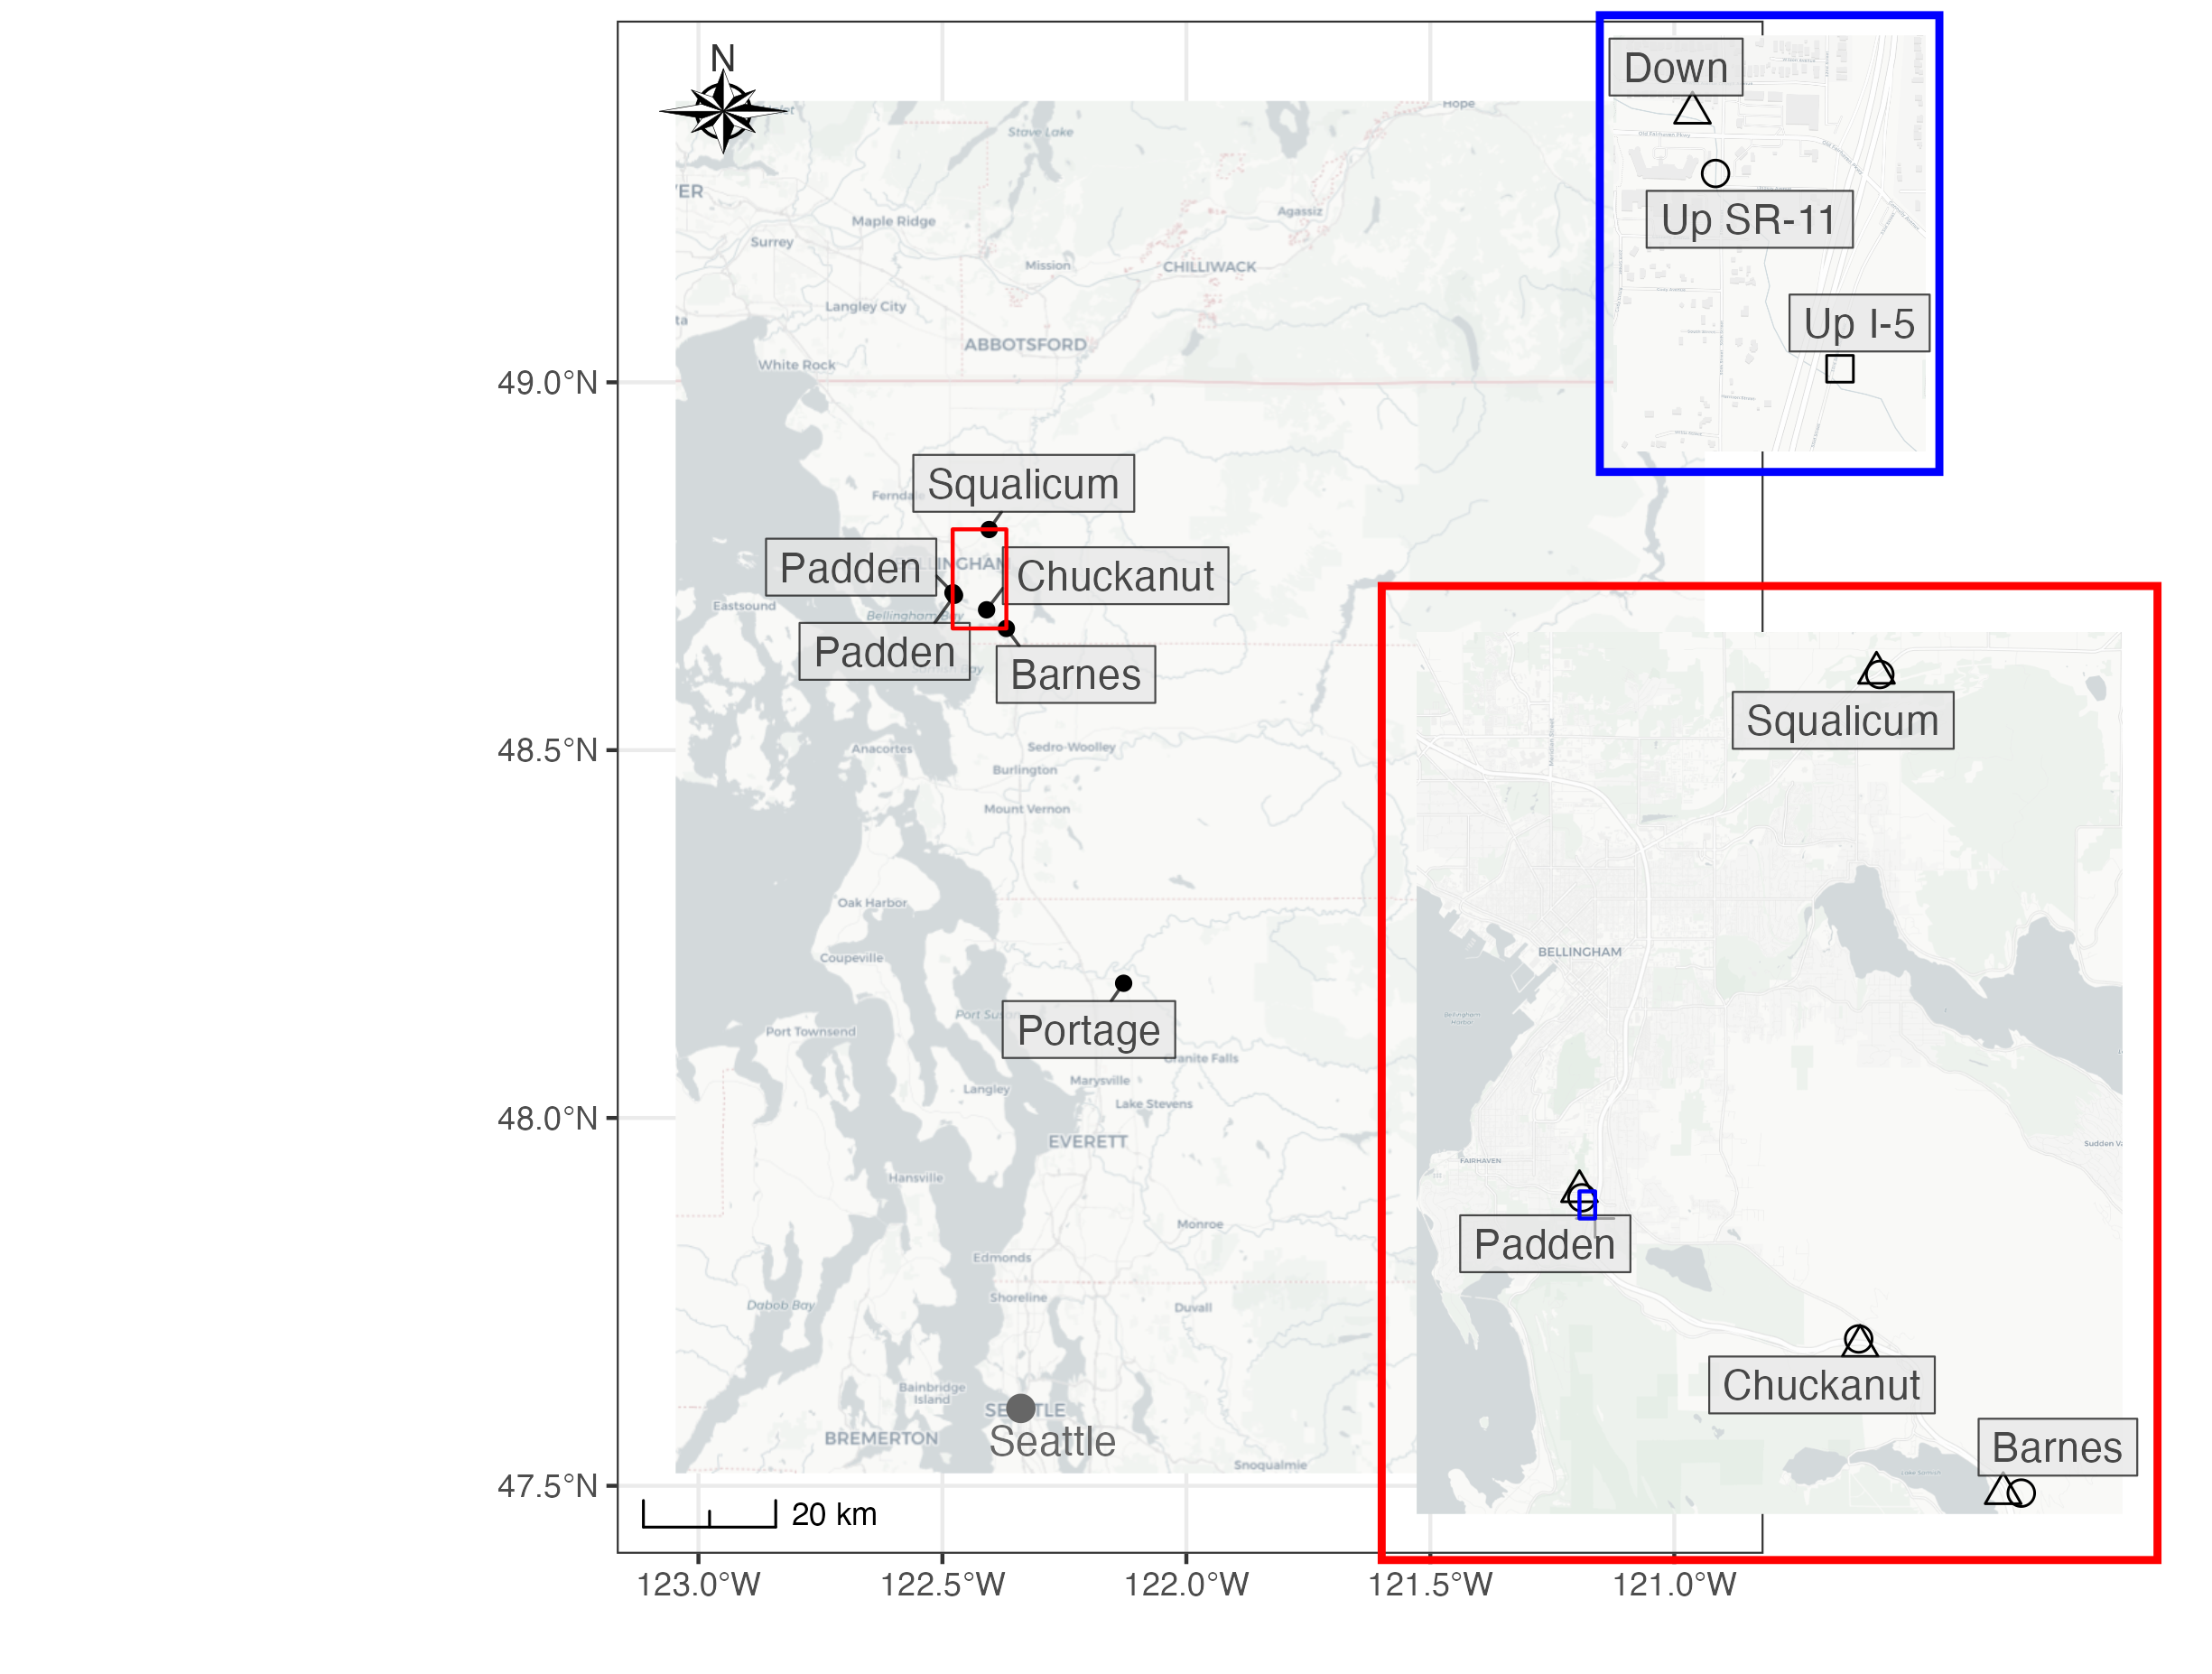
\includegraphics{../Output/Figures/SiteMap.png}
\caption{Map of sampling locations near Bellingham, Washington. \DIFaddbeginFL \DIFaddFL{In the
red subset, triangles designate the downstream sampling location and
circles designate the upstream sampling location. Padden Creek (the
treatment creek where the two culverts were replaced) is shown in the
blue subset where downstream is a triangle, upstream of the first
culvert (SR-11) is a circle, and upstream of the second culvert (I-5) is
a square.}\DIFaddendFL \label{fig:map}}

\end{figure}

The \DIFdelbegin \DIFdel{intervention (i.e., culvert replacement }\DIFdelend \DIFaddbegin \DIFadd{first culvert replacement (SR-11}\DIFaddend ) in Padden Creek occurred over
about two months and included the ``de-watering'' of the creek, removal
of the existing culvert, installation of the new culvert, and then the
``re-watering'' of the creek from late August 2021 to early October 2021
(Supplemental \DIFdelbegin \DIFdel{Figure 3). We }\DIFdelend \DIFaddbegin \DIFadd{Text 1; Figure S1.4). The second culvert replacement (I-5)
in Padden Creek was a much larger construction project, including
daylighting the creek and building a bridge under a large, five-lane
interstate. In-water work for the I-5 culvert replacement began in late
June 2022 and was completed in September 2022. By sampling before,
during, and after both construction events, we }\DIFaddend were then able to \DIFdelbegin \DIFdel{quantify }\DIFdelend \DIFaddbegin \DIFadd{isolate
}\DIFaddend the effect of the culvert replacement itself -- controlling for temporal
trends, background environmental variability, and sampling variability
-- using a \DIFdelbegin \DIFdel{Bayesian time-series model to jointly model salmon }\DIFdelend \DIFaddbegin \DIFadd{linear mixed effects model of }\DIFaddend eDNA abundances across creeks,
time points, sampling stations, and species.

Because salmonids are the primary species of management concern in these
creeks, we focus the present analysis on the four salmonid species most
common in our data: cutthroat trout (\emph{Oncorhynchus clarkii)}, coho
salmon (\emph{O. kisutch}), rainbow/steelhead trout (\emph{O. mykiss}),
and sockeye/kokanee salmon (\emph{O. nerka}). \DIFdelbegin \DIFdel{As further described
below, we surveyed the salmonid DNA present in each creek via eDNA
metabarcoding (targeting a region of the 12s mtDNA gene) and
complementary quantitative PCR (qPCR; targeting a region of the CytB
gene) for a reference species (cutthroat trout, }\emph{\DIFdel{O. clarkii}}%DIFAUXCMD
\DIFdel{),
which in combination yielded quantitative estimates for each fish
species throughout the study area.
}%DIFDELCMD < 

%DIFDELCMD < %%%
\DIFdelend Not all four salmonids are
expected to be found in all five of the creeks sampled. As documented by
WA Department of Fish and Wildlife SalmonScape
(\url{http://apps.wdfw.wa.gov/salmonscape/map.html}), all creeks contain
cutthroat trout, steelhead trout, and coho salmon. Barnes Creek is the
only creek documented to have kokanee salmon \DIFdelbegin \DIFdel{, which are
}\DIFdelend \DIFaddbegin \DIFadd{(a }\DIFaddend freshwater sub-type of
sockeye salmon\DIFdelbegin \DIFdel{that are not anadromous}\DIFdelend \DIFaddbegin \DIFadd{)}\DIFaddend . However, local spawner surveys conducted by the City of
Bellingham from 2015-2020 in Padden Creek documented kokanee salmon, as
well as the other three species \DIFdelbegin \DIFdel{and importantly, several unknown species of live and dead fish
and redds (nests dug by fish in gravel to deposit eggs) (}\DIFdelend \DIFaddbegin \DIFadd{(}\DIFaddend City of Bellingham 2015). \DIFdelbegin %DIFDELCMD < 

%DIFDELCMD < %%%
\DIFdelend The four
salmonid species in this study have different life histories and
behaviors that would impact when fish (and therefore eDNA
concentrations) occur in the creeks. \DIFdelbegin \DIFdel{For these four migratory salmonids,
the run timings vary for each species in the study area (Bellingham,
WA). Adult coastal cutthroat (}\emph{\DIFdel{O. clarkii}}%DIFAUXCMD
\DIFdel{) are documented to run
throughout the entire year, whereas coho salmon (}\emph{\DIFdel{O. kisutch}}%DIFAUXCMD
\DIFdel{) run
from September to December, sockeye salmon (}\emph{\DIFdel{O. nerka}}%DIFAUXCMD
\DIFdel{) run from
October to December, and steelhead trout (}\emph{\DIFdel{O. mykiss}}%DIFAUXCMD
\DIFdel{) run from
November to June. For migrating coho (}\emph{\DIFdel{O. kisutch}}%DIFAUXCMD
\DIFdel{) and steelhead
trout (}\emph{\DIFdel{O. mykiss}}%DIFAUXCMD
\DIFdel{), juveniles may be present in the creeks
year-round (Supplemental Figure 3). Using eDNA methods, it cannot be
determined if the DNA found is sourced from adult or juvenile animals.
}%DIFDELCMD < 

%DIFDELCMD < %%%
\DIFdelend Furthermore, three of the four
species in this study have both freshwater resident and saltwater
migrating behavior. \DIFdelbegin \DIFdel{Cutthroat trout
(}\emph{\DIFdel{O. clarkii}}%DIFAUXCMD
\DIFdel{) encompasses both non-migrating, resident trout in
the creeks and coastal run
cutthroat that migrate into Padden Creek from
saltwater (Bellingham Bay). Similarly, }\emph{\DIFdel{O. nerka}} %DIFAUXCMD
\DIFdel{includes both
anadromous sockeye salmon and freshwater resident kokanee salmon and
}\emph{\DIFdel{O. mykiss}} %DIFAUXCMD
\DIFdel{includes both anadromous steelhead trout and
non-migrating rainbow trout. Using eDNA, we cannot distinguish between
the migrating and non-migrating subspecies of }\emph{\DIFdel{O. clarkii}}%DIFAUXCMD
\DIFdel{,
}\emph{\DIFdel{O. nerka}}%DIFAUXCMD
\DIFdel{, and }\emph{\DIFdel{O. mykiss}}%DIFAUXCMD
\DIFdel{. }\DIFdelend \DIFaddbegin \DIFadd{For the fish exhibiting migratory behavior, the run
timings vary for each species in the study area (see Discussion and
Figure S1.4). }\DIFaddend Therefore, our eDNA concentrations might reflect
contributions from both migrating and non-migrating individuals at any
given time point in the dataset.

\hypertarget{water-sampling}{%
\subsubsection{Water Sampling}\label{water-sampling}}

\DIFdelbegin \DIFdel{We collected water samples monthly between }\DIFdelend \DIFaddbegin \DIFadd{From }\DIFaddend March 2021 \DIFdelbegin \DIFdel{and }\DIFdelend \DIFaddbegin \DIFadd{to }\DIFaddend February 2022\DIFdelbegin \DIFdel{in each of five salmonid-bearing creeks in northwest Washington State, USA (Figure \ref{fig:map}). We sampled each stream above and below
under-road culverts. }\DIFdelend \DIFaddbegin \DIFadd{, all five creeks were sampled monthly
(n=12). Monthly sampling continued in Portage Creek, Padden Creek, and
Squalicum Creek through August 2022, with one additional sampling point
in December 2022 (n=19). }\DIFaddend At each sampling station (\DIFdelbegin \DIFdel{N=2, }\DIFdelend upstream and
downstream of a culvert) at each creek\DIFdelbegin \DIFdel{(N = 5) in each month (N = 12)}\DIFdelend , we collected three 2-liter water
samples\DIFdelbegin \DIFdel{, for a total of 360 water
samples}\DIFdelend . Samples were collected using \DIFdelbegin \DIFdel{Smith Root's }\DIFdelend \DIFaddbegin \DIFadd{an }\DIFaddend eDNA Backpack (\DIFaddbegin \DIFadd{Smith Root;
}\DIFaddend Thomas et al. \DIFaddbegin \DIFadd{(}\DIFaddend 2018)\DIFaddbegin \DIFadd{)}\DIFaddend , a portable pumping-and-filtering device set to
filter at 1 L/min at 82.7 kPa (12 psi). In some months, less than 2 L of
water was filtered due to clogging\DIFdelbegin \DIFdel{(min = 1.02 L, mean = 1.97 L, median = 2.01 L;
see Supplemental Figure 4)}\DIFdelend . Water samples were filtered using
single-use inlet tubes through 5\(\mu\)m self-preserving filters (Smith
Root, Vancouver, WA), which were then dried and kept at room temperature
until DNA extraction within 1 month of collection (Thomas et al. 2019).

Over the course of the \DIFdelbegin \DIFdel{year of }\DIFdelend sampling, water discharge varied from very low to
no flow in summer months to high flow in winter months (Figure
\DIFdelbegin \DIFdel{2). Thus, when considering eDNA concentrations at a sampling
site, we need to account for the large difference in water volume over
the course of the year-long time series. In other words, given the same
number of fish and a constant eDNA shedding rate, we would expect to see
higher concentrations of DNA in summer months and lower concentrations
in winter months due to dilution of eDNA
in higher water volumes just
from the difference in flow. Other eDNA time series datasets also
correct for discharge to present eDNA data as a mass flow rate
}%DIFDELCMD < {[}%%%
\DIFdel{mass/time}%DIFDELCMD < {]} %%%
\DIFdel{(Tillotson et al. 2018, Thalinger et al. 2019). Here, we
convert eDNA }\DIFdelend \DIFaddbegin \DIFadd{\ref{fig:flows}). We account for this dilution by converting eDNA
}\DIFaddend concentration {[}copies/\(\mu\)L{]} to an eDNA mass flow rate
{[}copies/s{]} by multiplying eDNA concentrations by discharge {[}L/s{]}
\DIFdelbegin \DIFdel{.
}%DIFDELCMD < 

%DIFDELCMD < %%%
\DIFdelend \DIFaddbegin \DIFadd{(Tillotson et al. 2018, Thalinger et al. 2019). }\DIFaddend Flow gauges maintained
by the United States Geological Survey (USGS) were used for Padden Creek
\DIFaddbegin \DIFadd{(USGS Gauge 12201905)}\DIFaddend , Chuckanut Creek \DIFaddbegin \DIFadd{(USGS Gauge 12201700)}\DIFaddend , and
Squalicum Creek (\DIFaddbegin \DIFadd{USGS Gauge 12204010;
}\DIFaddend \url{https://maps.waterdata.usgs.gov/mapper/index.html}; U. S.
Geological Survey (1994); \DIFdelbegin \DIFdel{Supplemental Figure 1). During the year }\DIFdelend \DIFaddbegin \DIFadd{Figure S1.1). Over the course }\DIFaddend of sampling, the
flow gauges at Chuckanut Creek and Squalicum Creek became inoperable
after a major flooding event. To find discharge rates for Chuckanut and
Squalicum Creeks, five years of historical data (2015-2020) were used to
generate a \DIFdelbegin \DIFdel{daily }\DIFdelend \DIFaddbegin \DIFadd{monthly }\DIFaddend averaged correction factor based on Padden Creek
\DIFdelbegin \DIFdel{. For the year of sampling (2021-2022), the
discharge rates used at Chuckanut and Squalicum Creeks were estimated
based on the correction factor from Padden Creek (Supplemental Figure
2}\DIFdelend \DIFaddbegin \DIFadd{(Supplemental Text 1, Figure S1.3}\DIFaddend ). No discharge data was available for
Portage Creek or Barnes Creek. Based on field sampling conditions, the
discharge from Padden Creek was used as a proxy for both Portage and
Barnes as they are in similarly sized watershed areas and land-cover
characteristics.
\DIFdelbegin \DIFdel{Though in the year
of sampling, the discharge in Padden Creek ranged from no metered flow
to 23 m\textsuperscript{3}/s, the discharge on the dates of sampling
only reached a maximum of 1.3 m\textsuperscript{3}/s.
}\DIFdelend 

\begin{figure}
\centering
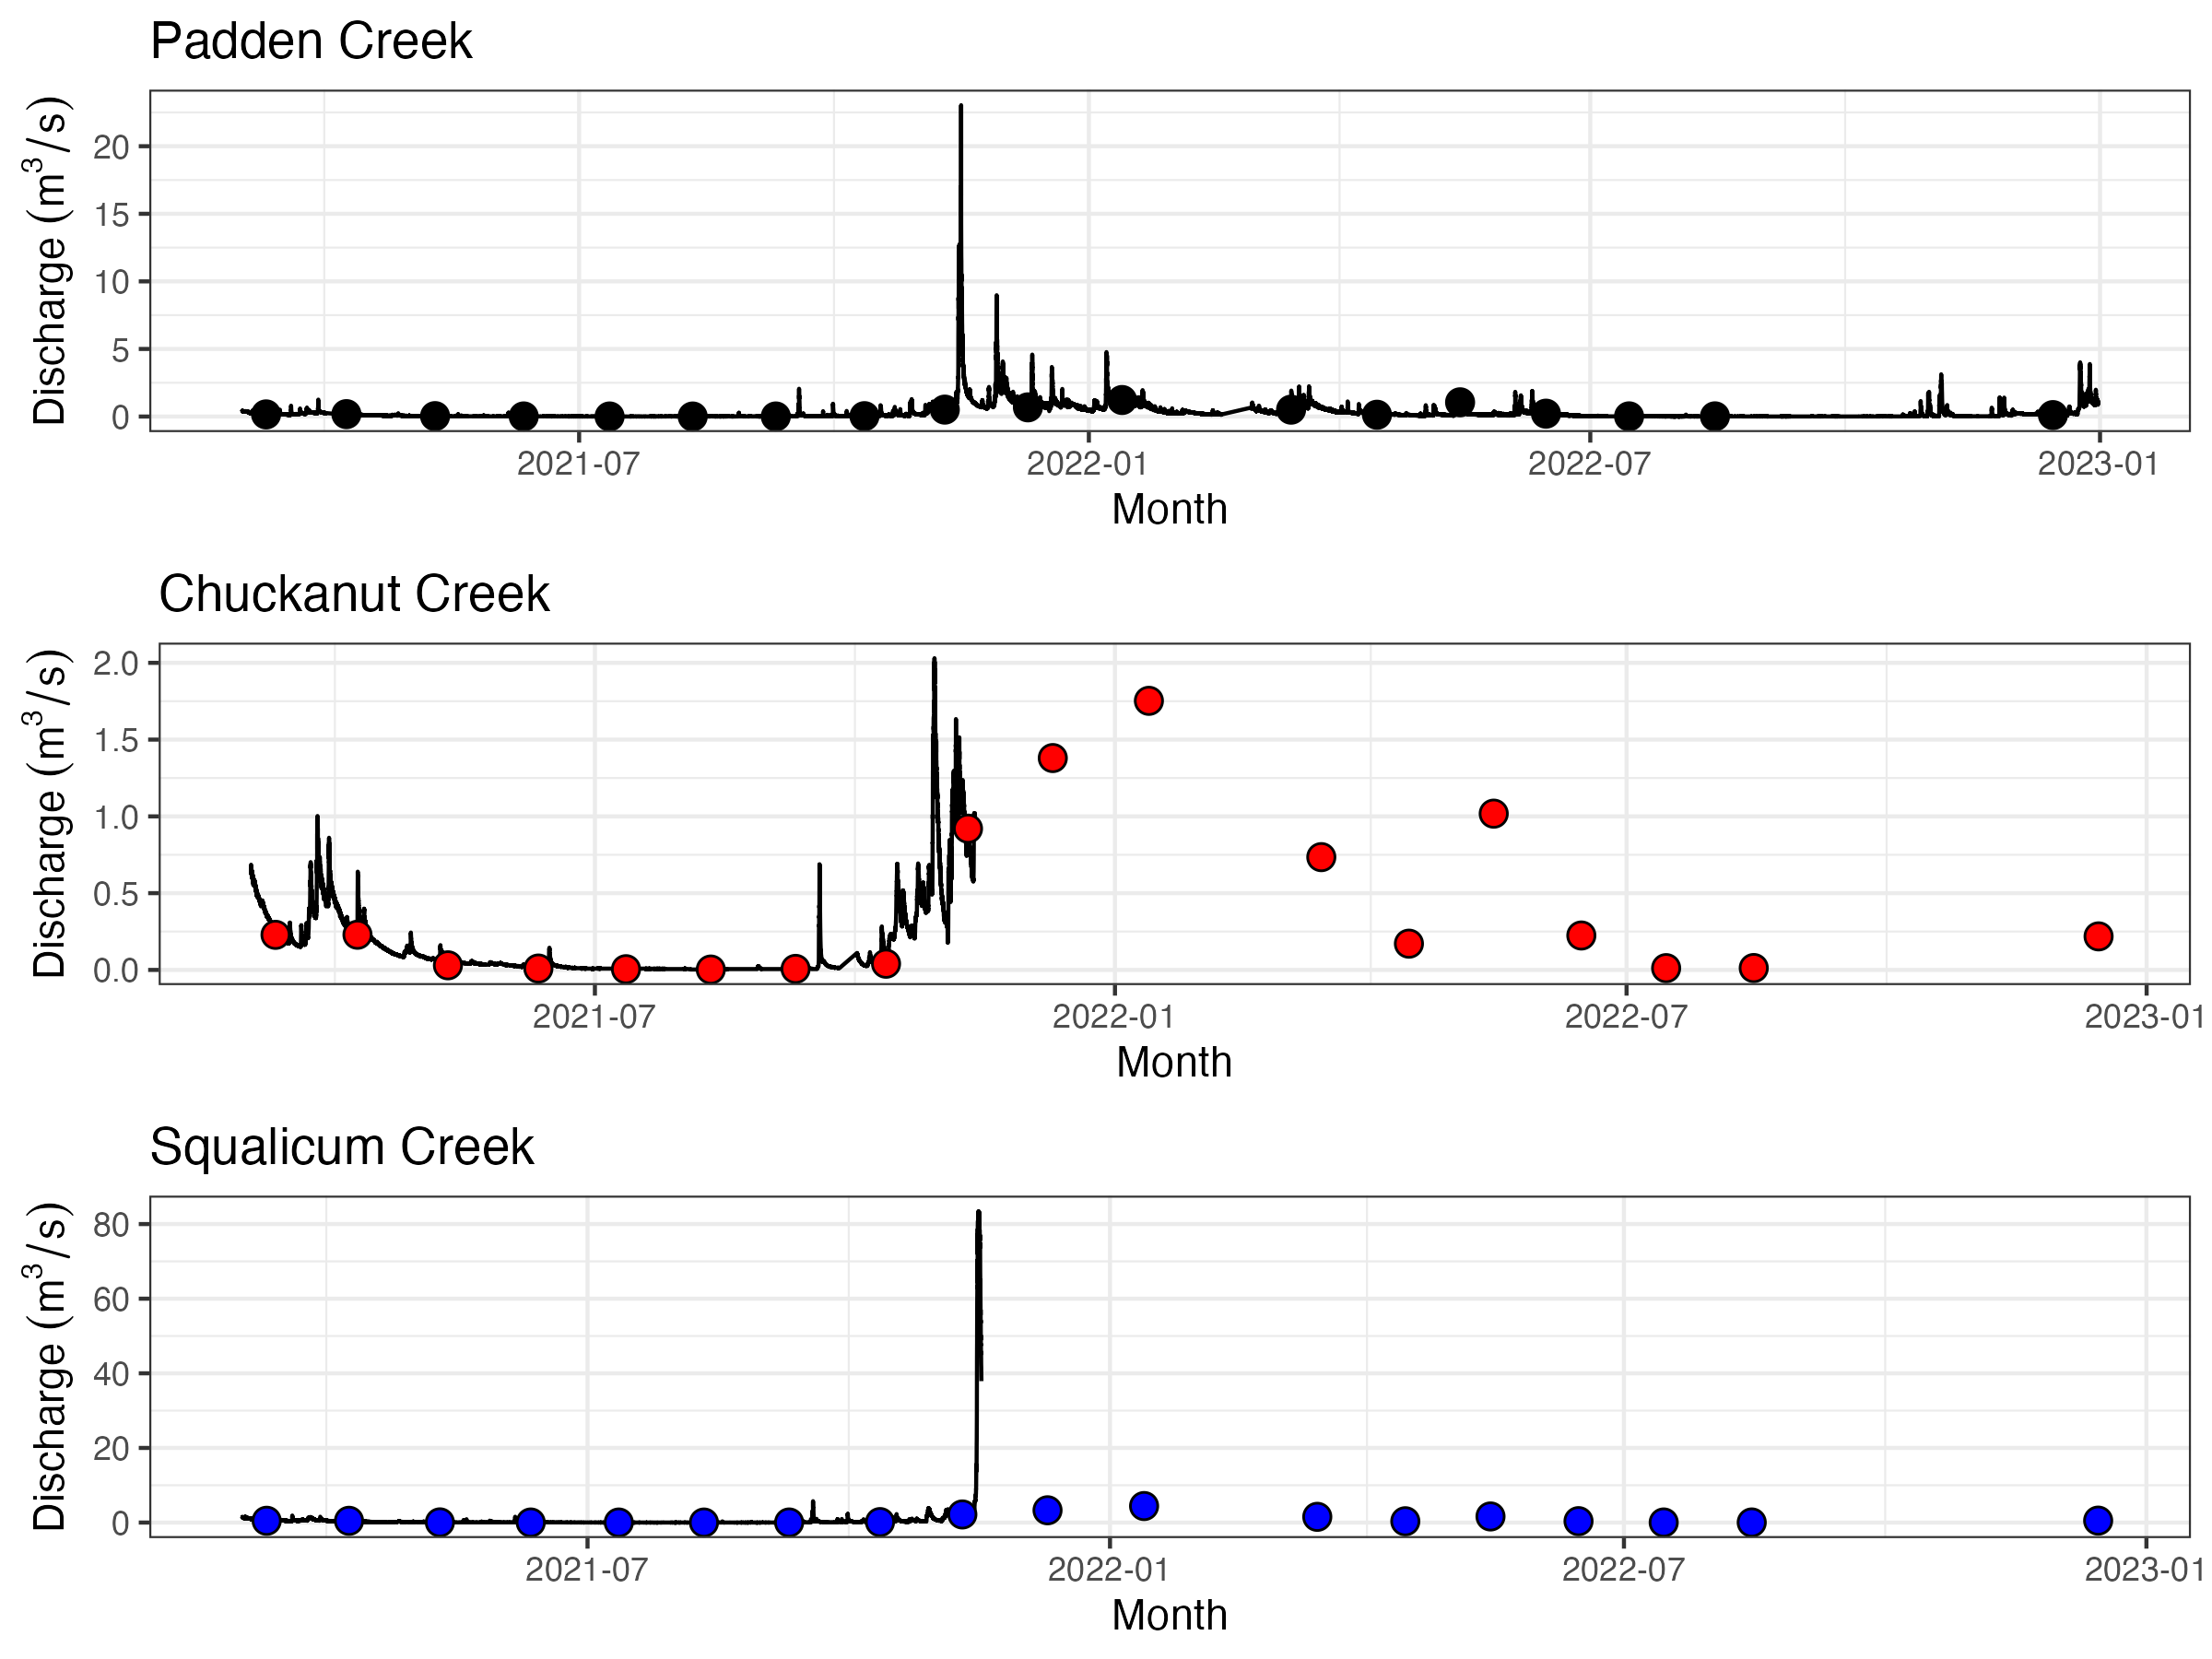
\includegraphics{../Output/Figures/flow_gauges.png}
\caption{Discharge (m\textsuperscript{3}/s) in Padden \DIFaddbeginFL \DIFaddFL{(USGS Gauge
12201905)}\DIFaddendFL , Chuckanut \DIFaddbeginFL \DIFaddFL{(USGS Gauge 12201700)}\DIFaddendFL , and Squalicum \DIFaddbeginFL \DIFaddFL{(USGS Gauge
12204010) }\DIFaddendFL Creeks over the course of sampling. \DIFdelbeginFL \DIFdelFL{Open circles show the days
when sampling occurred. }\DIFdelendFL Gauges at Chuckanut and
Squalicum Creek went offline in November 2021 after a major storm event.
Portage Creek and Barnes Creek did not have stream gauges. \DIFdelbeginFL %DIFDELCMD < \label{fig:flows}}
%DIFDELCMD < \end{figure}
%DIFDELCMD < 

%DIFDELCMD < %%%
\DIFdel{Additionally, in the creek of interest, Padden Creek, rainbow trout
(}\emph{\DIFdel{O. mykiss}}%DIFAUXCMD
\DIFdel{) were stocked in Lake Padden, approximately 1.5 km
upstream of the sampling sites. Occasionally, cutthroat trout (}\emph{\DIFdel{O.
clarkii}}%DIFAUXCMD
\DIFdel{) and kokanee salmon (}\emph{\DIFdel{O. nerka}}%DIFAUXCMD
\DIFdel{) have been stocked in the
past as well. During the course of the study, a total of 10}\DIFdelend \DIFaddbegin \DIFadd{Circles
designate the day of sampling. For Padden Creek}\DIFaddend , \DIFdelbegin \DIFdel{000 rainbow
trout were stocked in April and May 2021 }\DIFdelend \DIFaddbegin \DIFadd{the nearest 15 minute
interval of flow was used. For Chuckanut }\DIFaddend and \DIFdelbegin \DIFdel{30}\DIFdelend \DIFaddbegin \DIFadd{Squalicum Creeks}\DIFaddend , \DIFdelbegin \DIFdel{000 kokanee salmon were
stocked in May 2021 (Supplemental Figure }\DIFdelend \DIFaddbegin \DIFadd{the
correction factor from five years of historical data from Padden Creek
was used (see methods section and Supplemental Figures 2 and
}\DIFaddend 3\DIFdelbegin \DIFdel{). Despite the stocking of
30,000 kokanee salmon in May in Lake Padden, }\emph{\DIFdel{O. nerka}} %DIFAUXCMD
\DIFdel{was only
detected by metabarcoding in March 2021, August 2021, and then November
2021 through February 2022 (see results below). Importantly, this
suggests that Lake Padden is far enough upstream that the eDNA signal at
the sampling sites by the culvert is not a result of stocking the lake
1.5 km upstream (see discussion for more information).
}\DIFdelend \DIFaddbegin \DIFadd{).}\label{fig:flows}}

\end{figure}
\DIFaddend 

\hypertarget{dna-extraction-amplification-sequencing}{%
\subsubsection{DNA Extraction, Amplification,
Sequencing}\label{dna-extraction-amplification-sequencing}}

All molecular work prior to sequencing was performed at the University
of Washington. \DIFdelbegin \DIFdel{Bench-tops were cleaned with 10\% bleach for 10 minutes
and then wiped with 70\% ethanol. Molecular work was separated onto pre-
and post-PCR benches; all DNA extractions and PCR preparation was conducted on a bench where no PCR product was handled. DNA was extracted from half of each filter }\DIFdelend \DIFaddbegin \DIFadd{Details of the molecular work can be found in
Supplemental Text 1. Briefly, DNA was extracted off filters }\DIFaddend using a
Qiashredder column (Qiagen, USA) and the \DIFdelbegin \DIFdel{DNEasy }\DIFdelend \DIFaddbegin \DIFadd{DNeasy }\DIFaddend Blood and Tissue Kit
(Qiagen, USA) with an overnight incubation (Supplemental Text 1, Thomas
et al. (2019))\DIFdelbegin \DIFdel{, such that the
effective filtering effort was 1 L/sample; the remaining half of each
filter was archived at -20}%DIFDELCMD < \degree %%%
\DIFdel{C}\DIFdelend . Extracts were \DIFdelbegin \DIFdel{eluted in 100
\(\mu\)L of molecular grade water, quantified via Qubit (Invitrogen,
USA) and }\DIFdelend stored at -20\degree C until PCR
amplification within 2 months of extraction.

For \DIFdelbegin \DIFdel{the metabarcodingapproach}\DIFdelend \DIFaddbegin \DIFadd{metabarcoding}\DIFaddend , we targeted a \textasciitilde186 bp hypervariable
region of the mitochondrial DNA 12S rRNA gene for PCR amplification
(MiFish; Miya et al.~2015), but using modified primer sequences as given
in Praebel and Wangensteen (unpublished; via personal communication)\DIFdelbegin \DIFdel{and including the Illumina Nextera overhang sequences for
subsequent indexing.
The primers used were as follows: F 5'
}\emph{\DIFdel{TCGTCGGCAGCGTCAGATGTGTATAAGAGACAG}}%DIFAUXCMD
\DIFdel{GCCGGTAAAACTCGTGCCAGC 3', R 5'
}\emph{\DIFdel{GTCTCGTGGGCTCGGAGATGTGTATAAGAGACAG}}%DIFAUXCMD
\DIFdel{CATAGTGGGGTATCTAATCCCAGTTTG 3'
(}\emph{\DIFdel{italics}} %DIFAUXCMD
\DIFdel{indicate Nextera overhang). The }\DIFdelend \DIFaddbegin \DIFadd{.
The primer sequences, }\DIFaddend final reaction recipe\DIFaddbegin \DIFadd{, }\DIFaddend and cycling conditions can
be found in Supplemental Text 1. Each month of samples was amplified on
a single plate with the addition of a no template control (NTC;
molecular grade water in lieu of template) and a positive control
(genomic DNA from kangaroo\DIFdelbegin \DIFdel{). After PCR amplification,
PCR }\DIFdelend \DIFaddbegin \DIFadd{, a species not present in the environment).
PCR }\DIFaddend products were visualized\DIFdelbegin \DIFdel{on a 1-2\% gel. If no band was present for
a given sample, a new amplification was attempted with extracts diluted 1:10 iteratively until a band was detected. PCR products were
}\DIFdelend \DIFaddbegin \DIFadd{, }\DIFaddend size-selected\DIFdelbegin \DIFdel{and cleaned using MagBind Beads (Omega Biotek, USA) at a sample:beads ratio of 1.2. Bead-cleaned PCR products were eluted in 30
\(\mu\)L of molecular grade water and quantified via Qubit (Invitrogen,
USA).
}%DIFDELCMD < 

%DIFDELCMD < %%%
\DIFdel{An indexing PCR reaction added a unique
index }\DIFdelend \DIFaddbegin \DIFadd{, and diluted iteratively if
inhibited. After cleaning, a second PCR amplification added unique
indices }\DIFaddend to each sample using Nextera indices (Illumina, USA) to allow
pooling multiple samples onto the same sequencing run (See Supplemental
Text 1 for details). Indexed PCR products were also size-selected and
\DIFdelbegin \DIFdel{purified using MagBind Beads
(Omega Biotek, USA) at a sample:beads ratio of 0.8. Bead-cleaned PCR
products were eluted in 30 \(\mu\)L of molecular grade water and
quantified via Qubit. Indexed and bead-cleaned products were normalized
before pooling into libraries, which were subsequently quantified via
Qubit and visualized on a Bioanalyzer (Agilent, USA) before }\DIFdelend \DIFaddbegin \DIFadd{visualized before pooling for }\DIFaddend sequencing. Samples were randomized in
3-month blocks and each block split across 3 sequencing runs \DIFaddbegin \DIFadd{to avoid
run effects}\DIFaddend , for a total of \DIFdelbegin \DIFdel{12 }\DIFdelend \DIFaddbegin \DIFadd{14 }\DIFaddend sequencing runs. The loading
concentration of each library was 4-8 pM and 5-20\% PhiX was included
depending on the composition of the run. Sequencing was conducted using
an Illumina Miseq with v3 2x300 chemistry at the NOAA Northwest
Fisheries Science Center and the University of Washington's Northwest
Genomics Center.

Here, we used mock communities to determine the species-specific
amplification efficiencies for each salmonid in the study. \DIFdelbegin \DIFdel{Briefly, we
}\DIFdelend \DIFaddbegin \DIFadd{We
}\DIFaddend constructed five communities with known proportions of starting DNA from
different species (total DNA as measured by Qubit). The communities
ranged from having a total of 12 to 20 species, but six salmonid species
were included in all five mock communities \DIFdelbegin \DIFdel{to have more information on
the amplification efficiencies of salmonids }\DIFdelend (Supplemental Table \DIFdelbegin \DIFdel{3}\DIFdelend \DIFaddbegin \DIFadd{2}\DIFaddend ). We
sequenced these communities using the same metabarcoding primers and
thermocycling conditions above and then determined the species-specific
amplification rates given the discrepancy between the known starting
proportion and the proportion of reads after sequencing. \DIFdelbegin \DIFdel{These }\DIFdelend \DIFaddbegin \DIFadd{The }\DIFaddend mock
community data were then used to correct the sequencing reads from the
environmental samples to estimate the starting DNA proportions of each
species in environmental samples, which is the metric of interest
(Figure 3, green boxes). This is the first application of the model to
correct eDNA data from water samples with mock community data as
described in Shelton et al. (2022) (see Supplemental Text 2 for more
information).

\hypertarget{bioinformatics}{%
\subsubsection{Bioinformatics}\label{bioinformatics}}

After sequencing, bioinformatic analyses were conducted in R (R Core
Team 2017). A more detailed description of the bioinformatics pipeline
is included in \DIFdelbegin \DIFdel{the supplement (Supplemental Text 1). }\DIFdelend \DIFaddbegin \DIFadd{Supplemental Text 1. }\DIFaddend Briefly, primer sequences were
removed using \DIFdelbegin \DIFdel{Cutadapt }\DIFdelend \DIFaddbegin \emph{\DIFadd{Cutadapt}} \DIFaddend (Version 1.18) (Martin 2011) before
\DIFdelbegin \DIFdel{dada2 }\DIFdelend \DIFaddbegin \emph{\DIFadd{dada2}} \DIFaddend (Callahan et al. 2016) trimmed, filtered, merged paired end
reads, and generated amplicon sequence variants (ASVs). Taxonomic
assignment was conducted via the \DIFdelbegin \DIFdel{insect }\DIFdelend \DIFaddbegin \emph{\DIFadd{insect}} \DIFaddend package (Wilkinson et al.
2018) using a tree generated by the developers for the MiFish primers
that was last updated in November 2018. Only species level assignments
from \DIFdelbegin \DIFdel{insect }\DIFdelend \DIFaddbegin \emph{\DIFadd{insect}} \DIFaddend were retained and ASVs not annotated or not annotated
to species level were then checked against the NCBI nucleotide database
using BLAST+ (Camacho et al. 2009). Query sequences that matched a
single species at \textgreater95\% identity were retained.

\DIFdelbegin \DIFdel{In total, sequencing runs generated \textasciitilde42 million reads
across all environmental samples (12 months x 2 stations x 5 creeks x 3
biological replicates = 360 filters) and 27 mock community samples (3
communities x 9 replicates }%DIFDELCMD < {[}%%%
\DIFdel{6 even, 3 skewed proportions}%DIFDELCMD < {]}%%%
\DIFdel{) for
calibration (see below). After quality-filtering and merging all runs,
\textasciitilde33 million reads remained from \textasciitilde21,000
amplicon sequence variants (ASVs) in the environmental samples, of which
\textasciitilde81\% of reads and \textasciitilde2\% of ASVs were
annotated to species level (per sample: mean = 78\%, median = 88\%, min
= 0\%, max = 99.99\% of reads annotated). We only focus on the
metabarcoding data from four salmonids for the remainder of this paper.
The four salmonids represent \textasciitilde55\% of all environmental
reads and \textasciitilde68\% of the annotated reads found in
environmental samples.
}%DIFDELCMD < 

%DIFDELCMD < %%%
\DIFdel{In the mock community samples, 98.7\% of the \textasciitilde5 million
reads after quality filtering were annotated to species level.
Importantly, the target salmonid ASVs in the mock communities were found
in environmental samples, unambiguously linking the taxa in calibration
samples with those in environmental samples. The most common salmonid
species found in the environmental samples was }\emph{\DIFdel{O. clarkii}}
%DIFAUXCMD
\DIFdel{(cutthroat trout), which was found in \textasciitilde90\% of samples,
followed by }\emph{\DIFdel{O. kisutch}} %DIFAUXCMD
\DIFdel{found in \textasciitilde60\% of samples,
then }\emph{\DIFdel{O. mykiss}} %DIFAUXCMD
\DIFdel{found in \textasciitilde40\% of samples, and
finally }\emph{\DIFdel{O. nerka}} %DIFAUXCMD
\DIFdel{found in \textasciitilde5\% of samples. Not only
was }\emph{\DIFdel{O. clarkii}} %DIFAUXCMD
\DIFdel{found in the majority of environmental samples,
but also \textasciitilde63\% of samples across all times, creeks, and
stations had at least 50\% of reads assigned to }\emph{\DIFdel{O. clarkii}}%DIFAUXCMD
\DIFdel{.
}%DIFDELCMD < 

%DIFDELCMD < %%%
\DIFdelend \hypertarget{quantitative-pcr-and-inhibition-testing}{%
\subsubsection{Quantitative PCR and Inhibition
Testing}\label{quantitative-pcr-and-inhibition-testing}}

We quantified cutthroat trout (\emph{O. clarkii}) DNA in each sample,
targeting a 114 bp fragment of the cytochrome b gene with a qPCR assay
(Duda et al. 2021). The primer/probe sequences\DIFdelbegin \DIFdel{were: F 5'
CCGCTACAGTCCTTCACCTTCTA 3', R 5' GATCTTTGTATGAGAAGTAAGGATGGAA 3', P 5'
6FAM-TGAGACAGGATCCAAC-MGB-NFQ 3'. The qPCR assay was multiplexed with
TaqMan Exogenous Internal Positive Control Reagents (EXO-IPC) (Applied
Biosystems, USA) to check for the presence of PCR inhibitors (Duda et
al. 2021). The EXO-IPC mix includes the primers and probe for the
EXO-IPC DNA, with the probe having a VIC reporter, allowing it to be
multiplexed with the }\emph{\DIFdel{O. clarkii}} %DIFAUXCMD
\DIFdel{assay, which has a FAM reporter.
Each DNA sample was run in triplicate; the final recipe}\DIFdelend \DIFaddbegin \DIFadd{, final recipe, }\DIFaddend and
thermocycling conditions can be found in Supplemental Text 1. \DIFdelbegin \DIFdel{All qPCRs
were conducted on an Applied Biosystems StepOnePlus thermocycler.
}%DIFDELCMD < 

%DIFDELCMD < %%%
\DIFdel{Each plate included a 8-point standard curve created using synthetic DNA
(gBlocks) at the following concentrations: 100,000 copies/\(\mu\)L,
10,000 copies/\(\mu\)L, 1,000 copies/\(\mu\)L, 100 copies/\(\mu\)L, 10
copies/\(\mu\)L, 5 copies/\(\mu\)L, 3 copies/\(\mu\)L, 1 copy/\(\mu\)L
Additionally, six no template controls (NTCs) were included on each
plate: 3 with the IPC DNA mix and 3 with molecular grade water instead
of template or IPC DNA mix. Plates were re-run if efficiency as
determined by the standard curve was outside of the range of 90-110\%.
}%DIFDELCMD < 

%DIFDELCMD < %%%
\DIFdel{To check for inhibition , the
cycle threshold (Ct) value determined for
the }\DIFdelend \DIFaddbegin \DIFadd{Each DNA
sample was run in triplicate and was checked for inhibition using the
}\DIFaddend EXO-IPC assay \DIFdelbegin \DIFdel{from the NTC was compared to the Ct value for the
EXO-IPC assay in each of the environmental samples. If the Ct value was
\textgreater0.5 Ct values from the mean Ct for the NTCs, the sample was
deemed inhibited and diluted 1:10 and re-assayed until the Ct value fell
within the accepted range. }\DIFdelend \DIFaddbegin \DIFadd{(Applied Biosystems). }\DIFaddend The majority of environmental
samples (\DIFdelbegin \DIFdel{65}\DIFdelend \DIFaddbegin \DIFadd{60}\DIFaddend \%) were inhibited and accordingly diluted for analysis. In
\DIFdelbegin \DIFdel{75}\DIFdelend \DIFaddbegin \DIFadd{80}\DIFaddend \% of inhibited samples, a 1:10 dilution \DIFaddbegin \DIFadd{or less }\DIFaddend remedied the
inhibition, but some samples \DIFaddbegin \DIFadd{(11\%) }\DIFaddend required dilution by a factor of up
to \DIFdelbegin \DIFdel{1000 (Supplemental Figure
5) .
}\DIFdelend \DIFaddbegin \DIFadd{1000. Each plate included a 8-point standard curve created using
synthetic DNA (gBlocks) ranging from 1 to 100,000 copies/\(\mu\)L and
six no template controls (NTCs) were included on each plate with
molecular grade water instead of template. All qPCRs were conducted on
an Applied Biosystems StepOnePlus thermocycler.
}\DIFaddend 

All qPCR data was processed in R using Stan (Stan Development Team
2022), relating environmental samples to the standard curve via a linear
model (Figure \ref{fig:conceptualfig}, blue boxes\DIFaddbegin \DIFadd{; Figure S2.1}\DIFaddend ). We
amended the standard linear regression model to more realistically
capture the behavior of qPCR observations, accommodating non-detections
as a function of underlying DNA concentration, and letting the standard
deviation vary with the mean (lower-concentration samples had more
uncertainty). See McCall et al. (2014) and Shelton et al. (2019) for
similar models; see Supplemental Text 2 for full statistical details.
Subsequent analysis corrected for sample-specific dilution if found
inhibited and corrected for any variation in water-volume filtered
during sample collection. \DIFaddbegin \DIFadd{Samples with standard deviations between
technical replicates larger than 1.5 Ct values were removed from
analyses.
}\DIFaddend 

\hypertarget{quantitative-metabarcoding}{%
\subsubsection{Quantitative
Metabarcoding}\label{quantitative-metabarcoding}}

The intercalibration of the mock community samples demonstrated the rank
order of amplification efficiencies for salmonids (Supplemental Figures
\DIFdelbegin \DIFdel{14 and 15). }\DIFdelend \DIFaddbegin \DIFadd{10 and 11). Cutthroat trout (}\DIFaddend \emph{O. clarkii}\DIFdelbegin \DIFdel{and }\DIFdelend \DIFaddbegin \DIFadd{) and sockeye/kokanee
salmon (}\DIFaddend \emph{O. nerka}\DIFaddbegin \DIFadd{) }\DIFaddend had similar amplification efficiencies, both of
which were higher than \DIFaddbegin \DIFadd{rainbow/steelhead trout (}\DIFaddend \emph{O. mykiss}\DIFdelbegin \DIFdel{and }\DIFdelend \DIFaddbegin \DIFadd{) and
coho salmon (}\DIFaddend \emph{O. kisutch}\DIFaddbegin \DIFadd{)}\DIFaddend , which had the lowest amplification
efficiency. Calibrated metabarcoding analysis yielded quantitative
estimates of the proportions of species' DNA in environmental samples
prior to PCR. We then converted these proportions into absolute
abundances by expansion, using the qPCR results for our reference
species, \DIFaddbegin \DIFadd{cutthroat trout (}\DIFaddend \emph{O. clarkii}\DIFaddbegin \DIFadd{)}\DIFaddend . We estimated the total
amplifiable salmonid DNA in environmental sample \(i\) as
\DIFdelbegin \DIFdel{\(\text{DNA}_{\text{salmonid}_{i}} = \frac{\text{qPCR}_{\text{reference}_{i}}}{\text{Proportion}_{\text{reference}_{i}}}\),
}\DIFdelend \DIFaddbegin \DIFadd{\(\text{C}_{\text{amplifiable}_{i}} = \frac{\text{C}_{\text{qPCR reference}_{i}}}{\text{Proportion}_{\text{reference}_{i}}}\),
where C has units of }{[}\DIFadd{DNA copies/uL}{]} \DIFaddend and then expanded species'
proportions into absolute concentrations by multiplying these
sample-specific total concentrations by individual species' proportions,
such that for species \(j\) in sample \(i\),
\DIFdelbegin \DIFdel{\(\text{DNA}_{i,j} = \text{DNA}_{\text{salmonid}_{i}} * \text{Proportion}_{i,j}\)}\DIFdelend \DIFaddbegin \DIFadd{\(\text{C}_{i,j} = \text{C}_{\text{amplifiable}_{i}} * \text{Proportion}_{i,j}\)}\DIFaddend .
Here, we combine the modeled output of the qPCR model for \DIFdelbegin \emph{\DIFdel{O.
clarkii}} %DIFAUXCMD
\DIFdelend \DIFaddbegin \DIFadd{cutthroat
trout }\DIFaddend (Figure \ref{fig:conceptualfig} dashed blue box) and modeled
proportions of salmonid DNA from metabarcoding (Figure
\ref{fig:conceptualfig} dashed green box). \DIFdelbegin \DIFdel{Though }\DIFdelend \DIFaddbegin \DIFadd{Although }\DIFaddend in the future this
could be used as a joint model, here the precision of our modeled
estimates were very high such that we used the mean of the posterior
estimates from each model to move forward as input to the time series
model (Figure \ref{fig:conceptualfig} dashed purple box; see
Supplemental Text 2 for more details). \DIFdelbegin %DIFDELCMD < 

%DIFDELCMD < %%%
\DIFdelend Finally, due to the range of
water discharge over the course of the year, we converted from DNA
concentration {[}copies/L{]} to a mass flow rate {[}copies/s{]} after
multiplying by the discharge of each creek {[}m\textsuperscript{3}/s{]}
(Figure \ref{fig:conceptualfig}, solid purple boxes).

\begin{figure}
\centering
\DIFdelbeginFL %DIFDELCMD < 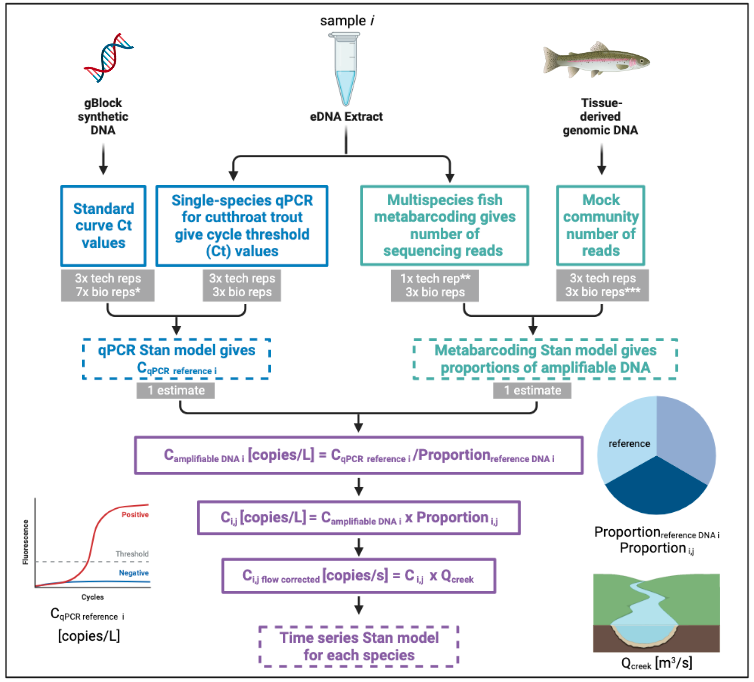
\includegraphics{../Output/Figures/conceptual_figure.png}
%DIFDELCMD < %%%
\DIFdelendFL \DIFaddbeginFL 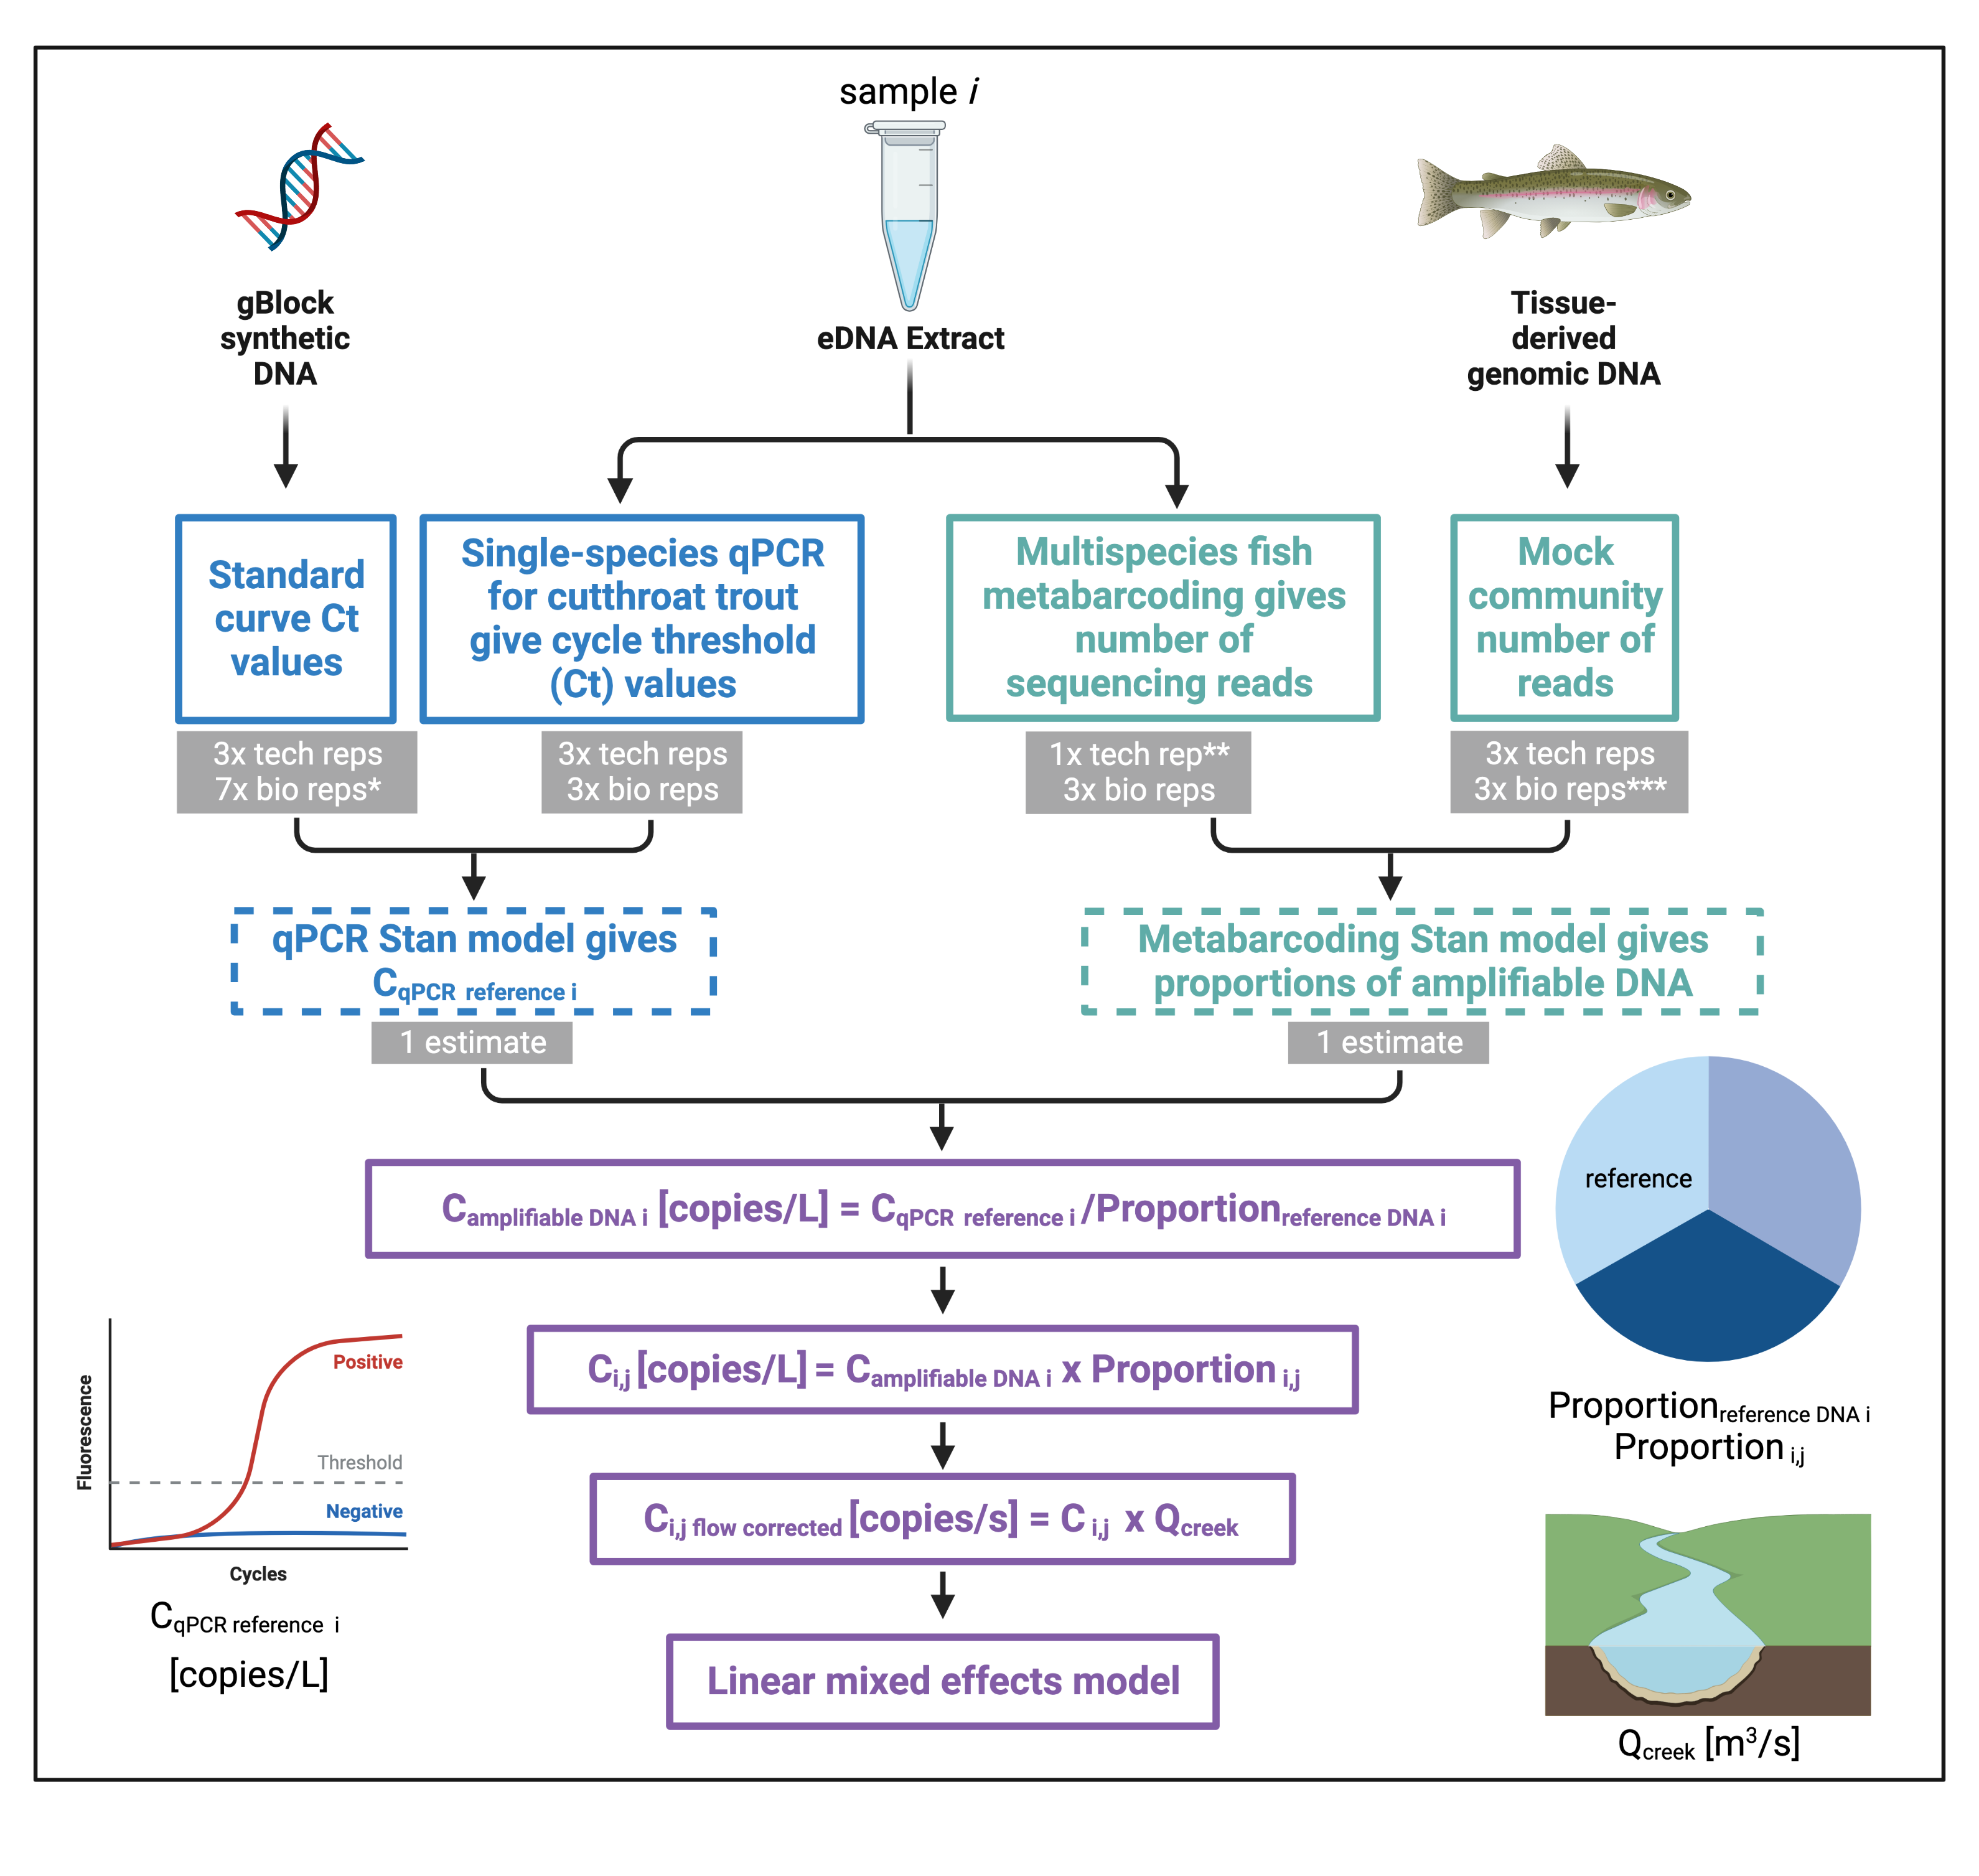
\includegraphics{../Output/Figures/NGN_Fig3.png}
\DIFaddendFL \caption{Conceptual figure of different datasets and models used for
analyses. * indicates that here, biological replicates are different
dilutions of the synthetic gBlock. ** indicates that for most samples,
only one technical replicate was sequenced but for one sample per
sampling month, three \DIFdelbeginFL \DIFdelFL{techincal }\DIFdelendFL \DIFaddbeginFL \DIFaddFL{technical }\DIFaddendFL replicates were sequenced to check for
consistency across replicates. *** indicates that here, the three
biological replicates indicate three different mock communities with
varying species compositions, but all containing the four salmonids of
interest. \DIFaddbeginFL \DIFaddFL{Created with BioRender.com.}\DIFaddendFL \label{fig:conceptualfig}}

\end{figure}

\hypertarget{estimating-the-effects-of-culvert-replacement-and-of-culverts-themselves}{%
\subsubsection{Estimating the Effects of Culvert Replacement and of
Culverts
Themselves}\label{estimating-the-effects-of-culvert-replacement-and-of-culverts-themselves}}

\DIFdelbegin \DIFdel{Consistent with the asymmetrical BACI study design, we generated data
from our }\DIFdelend \DIFaddbegin \DIFadd{We sampled }\DIFaddend four control creeks as context against which to compare the
observations in Padden Creek, our treatment creek \DIFaddbegin \DIFadd{where the two culverts
were being replaced. At a given station in a given creek, some DNA
concentration exists for each species. For simplicity, we focus on a
single species and a single station (downstream or upstream) for the
moment. Our observations of the (log) DNA concentration in creek \(i\)
at time \(t\) are distributed as
\(Y_{i,t} \sim \mathcal{N}(\mu_{i,t},\,\sigma^{2})\). More complex
versions of the model may let \(\sigma\) vary across creeks, time
points, species, or with environmental covariates of interest}\DIFaddend .
\DIFdelbegin \DIFdel{Recognizing that
these observations are autocorrelated in time, we use an AR(1) autocorrelation model , implemented in Stan via R, to capture the
observed temporal trends.
}\DIFdelend 

We \DIFdelbegin \DIFdel{observe the log-DNA concentration }\DIFdelend \DIFaddbegin \DIFadd{are interested in how the DNA concentration changes over time, so we
assert that the expected value of DNA in a creek at time \(t\)}\DIFaddend ,
\DIFdelbegin \DIFdel{\(Y\), for a given species in a
given sample as a random variable drawn from a normal distribution with
mean \(\mu\) and observation variance \(\sigma^2\)}\DIFdelend \DIFaddbegin \DIFadd{\(\mu_{i,t}\), depends upon its time point, in some way. We considered
three ways of modeling the salmonid eDNA data, each in a Bayesian
framework, but each treating non-independence among time points somewhat
differently:
}

\begin{itemize}
\item
  \DIFadd{A linear auto-regressive (AR(1)) model, written in~}\texttt{\DIFadd{stan}}\DIFaddend . For
  each species \DIFdelbegin \DIFdel{\(j\)}\DIFdelend \DIFaddbegin \DIFadd{in each creek}\DIFaddend , the expected \DIFdelbegin \DIFdel{log-DNA concentration \(\mu\) at time \(t\) in creek
\(i\) at station \(d\) }\DIFdelend \DIFaddbegin \DIFadd{concentration of eDNA of each
  month }\DIFaddend is a linear function of the \DIFdelbegin \DIFdel{DNA concentration for
the same creek/station at \(t-1\). }\DIFdelend \DIFaddbegin \DIFadd{expected value from the previous
  month. Within a species, the monthly autoregressive parameters are
  shared across creeks.
}\item
  \DIFadd{A generalized additive model (GAM), written in~}\texttt{\DIFadd{brms}}\DIFadd{~(which
  itself writes a~}\texttt{\DIFadd{stan}}\DIFadd{~model). For each species in each creek,
  an independent set of spline (weighting) parameters describes the
  temporal trends in expected eDNA concentration; the number of spline
  knots is shared across species and creeks.
}\item
  \DIFadd{A linear mixed-effects (LME) model, written in~}\texttt{\DIFadd{rstanarm}}\DIFadd{. For
  each species in each creek, sampling month is treated as a random
  effect. Each species-creek-month effect is treated as an independent
  draw from a common distribution.~
}\end{itemize}
\DIFaddend 

\DIFdelbegin \begin{align*}\DIFdel{%DIFDELCMD < \label{eqn:ts}%%%
Y_{i,t,d} }&\DIFdel{\sim \mathcal{N}(\mu_{i,t,d},\,\sigma^{2})}\\
\DIFdel{\mu_{i,t,d} }&\DIFdel{= \alpha_{i,t} + \epsilon_{i,t,d} + \eta_{i,t,d}}\\
\DIFdel{\epsilon_{i,t,d} }&\DIFdel{\sim \mathcal{N}(\beta\mu_{i,t-1,d},\, \phi^2)
}\end{align*}%DIFAUXCMD
\DIFdelend \DIFaddbegin \DIFadd{Ultimately, the three models yielded very similar results (Figure S2.2),
and the LME model proved simplest and most flexible insofar as it could
easily handle datasets with uneven sets of observations -- for example,
cases in which a species was detected downstream of a barrier, but not
upstream.
}\DIFaddend 

\DIFdelbegin \DIFdel{Intercept \(\alpha\) varies by time, creek, and species , capturing
creek-level deviations from the
  previous time-step.
The autoregression
term \(\epsilon\) is itself a random
  variable drawn from a normal
distributionwith expected value \(\beta\mu_{i,t-1,d}\) and process
variance \(\phi^2\), such that the species-specific slope term \(\beta\)
estimates the degree of autocorrelation in log-DNA concentration between
one time-step and the next.
The model shares information across creeks
and time-points via \(\beta\). }\DIFdelend \DIFaddbegin \DIFadd{In }\texttt{\DIFadd{R}} \DIFadd{code using }\texttt{\DIFadd{rstanarm}}\DIFadd{, this model is coded as
}\DIFaddend 

\DIFdelbegin \DIFdel{Finally, \(\eta\) captures the difference in log-DNA concentration
between upstream and downstream stations within a creek; we set
\(\eta_{d = 1} = 0\) such that the value of \(\eta_{d = 2}\) explicitly
captures the effect of the culvert within a given creek at a given time. The effect of construction in our focal Padden Creek, then, is the change in \(\eta\) after construction versus prior to construction.
We
fit this model in a Bayesian framework using moderately informative
priors on all parameters, and confirmed model convergence
(\(\hat{R} < 1.01\))across 3 chains and 2500 model iterations. See
statistical supplement (Supplemental Text 2) for prior values, diagnostics, and full model details.
}\DIFdelend \DIFaddbegin \DIFmodbegin
\begin{DIFverbatim}[alsolanguage=DIFcode]
%DIF > stan_glmer(log(observed) ~ (1 + time_idx|creek:species) + (1|station:creek:species:time_idx)
\end{DIFverbatim}
\DIFmodend
\DIFaddend 

\DIFaddbegin \DIFadd{See Supplemental Text 2 for more details on the linear mixed-effects
model. ~
}

\DIFaddend \hypertarget{results}{%
\subsection{Results}\label{results}}

\hypertarget{metabarcoding-and-quantitative-pcr}{%
\subsubsection{Metabarcoding and Quantitative
PCR}\label{metabarcoding-and-quantitative-pcr}}

\DIFaddbegin \DIFadd{In total, we generated \textasciitilde52 million reads across all
environmental samples and 27 mock community samples (3 communities x 9
replicates }{[}\DIFadd{6 even, 3 skewed proportions}{]}\DIFadd{) for calibration (see
below). }\DIFaddend After \DIFaddbegin \DIFadd{quality-filtering and merging all runs, \textasciitilde45
million reads remained from \textasciitilde24,000 amplicon sequence
variants (ASVs) in the environmental samples, of which
\textasciitilde83\% of reads were annotated to species level (per
sample: mean = 82\%, median = 93\%, min = 0\%, max = 99.99\% of reads
annotated). We only focus on the metabarcoding data from four salmonids
for the remainder of this paper. The four salmonids represent
\textasciitilde54\% of all reads and \textasciitilde64\% of the
annotated reads found in environmental samples.
}

\DIFadd{In the mock community samples, 98.7\% of the \textasciitilde5 million
reads after quality filtering were annotated to species level.
Importantly, the target salmonid ASVs in the mock communities were found
in environmental samples, unambiguously linking the taxa in calibration
samples with those in environmental samples. The most common salmonid
species found in the environmental samples was cutthroat trout (}\emph{\DIFadd{O.
clarkii}}\DIFadd{), which was found in \textasciitilde85\% of samples, followed
by coho salmon (}\emph{\DIFadd{O. kisutch}}\DIFadd{) found in \textasciitilde62\% of
samples, then rainbow/steelhead trout (}\emph{\DIFadd{O. mykiss}}\DIFadd{) found in
\textasciitilde40\% of samples, and finally sockeye/kokanee salmon
(}\emph{\DIFadd{O. nerka}}\DIFadd{) found in \textasciitilde10\% of samples. Over half of
the samples across all times, creeks, and stations had at least 50\% of
reads assigned to cutthroat trout.
}

\DIFadd{After }\DIFaddend calibrating metabarcoding data using mock communities \DIFaddbegin \DIFadd{(See
Supplemental Texts 1 and 2)}\DIFaddend , we estimated the salmonid composition
across time points, creeks, and stations (\DIFdelbegin \DIFdel{Figure \ref{fig:qm}}\DIFdelend \DIFaddbegin \DIFadd{Figures \ref{fig:qm_controls}
and \ref{fig:qm_padden}}\DIFaddend ). The culvert in one control creek (Barnes)
appeared to be nearly a total barrier to salmonid passage, with salmonid
eDNA detected upstream of the culvert at only three time points, in
contrast to being detected at every time point in the downstream station
of the same creek. The other four creeks had no such pattern associated
with the culverts, suggesting that fish passage may have been possible
through the culverts, or that there were resident populations upstream
of the culverts.

\begin{figure}
\centering
\DIFdelbeginFL %DIFDELCMD < \includegraphics{../Output/Figures/20221123_proportions_after_qm.png}
%DIFDELCMD < %%%
\DIFdelendFL \DIFaddbeginFL 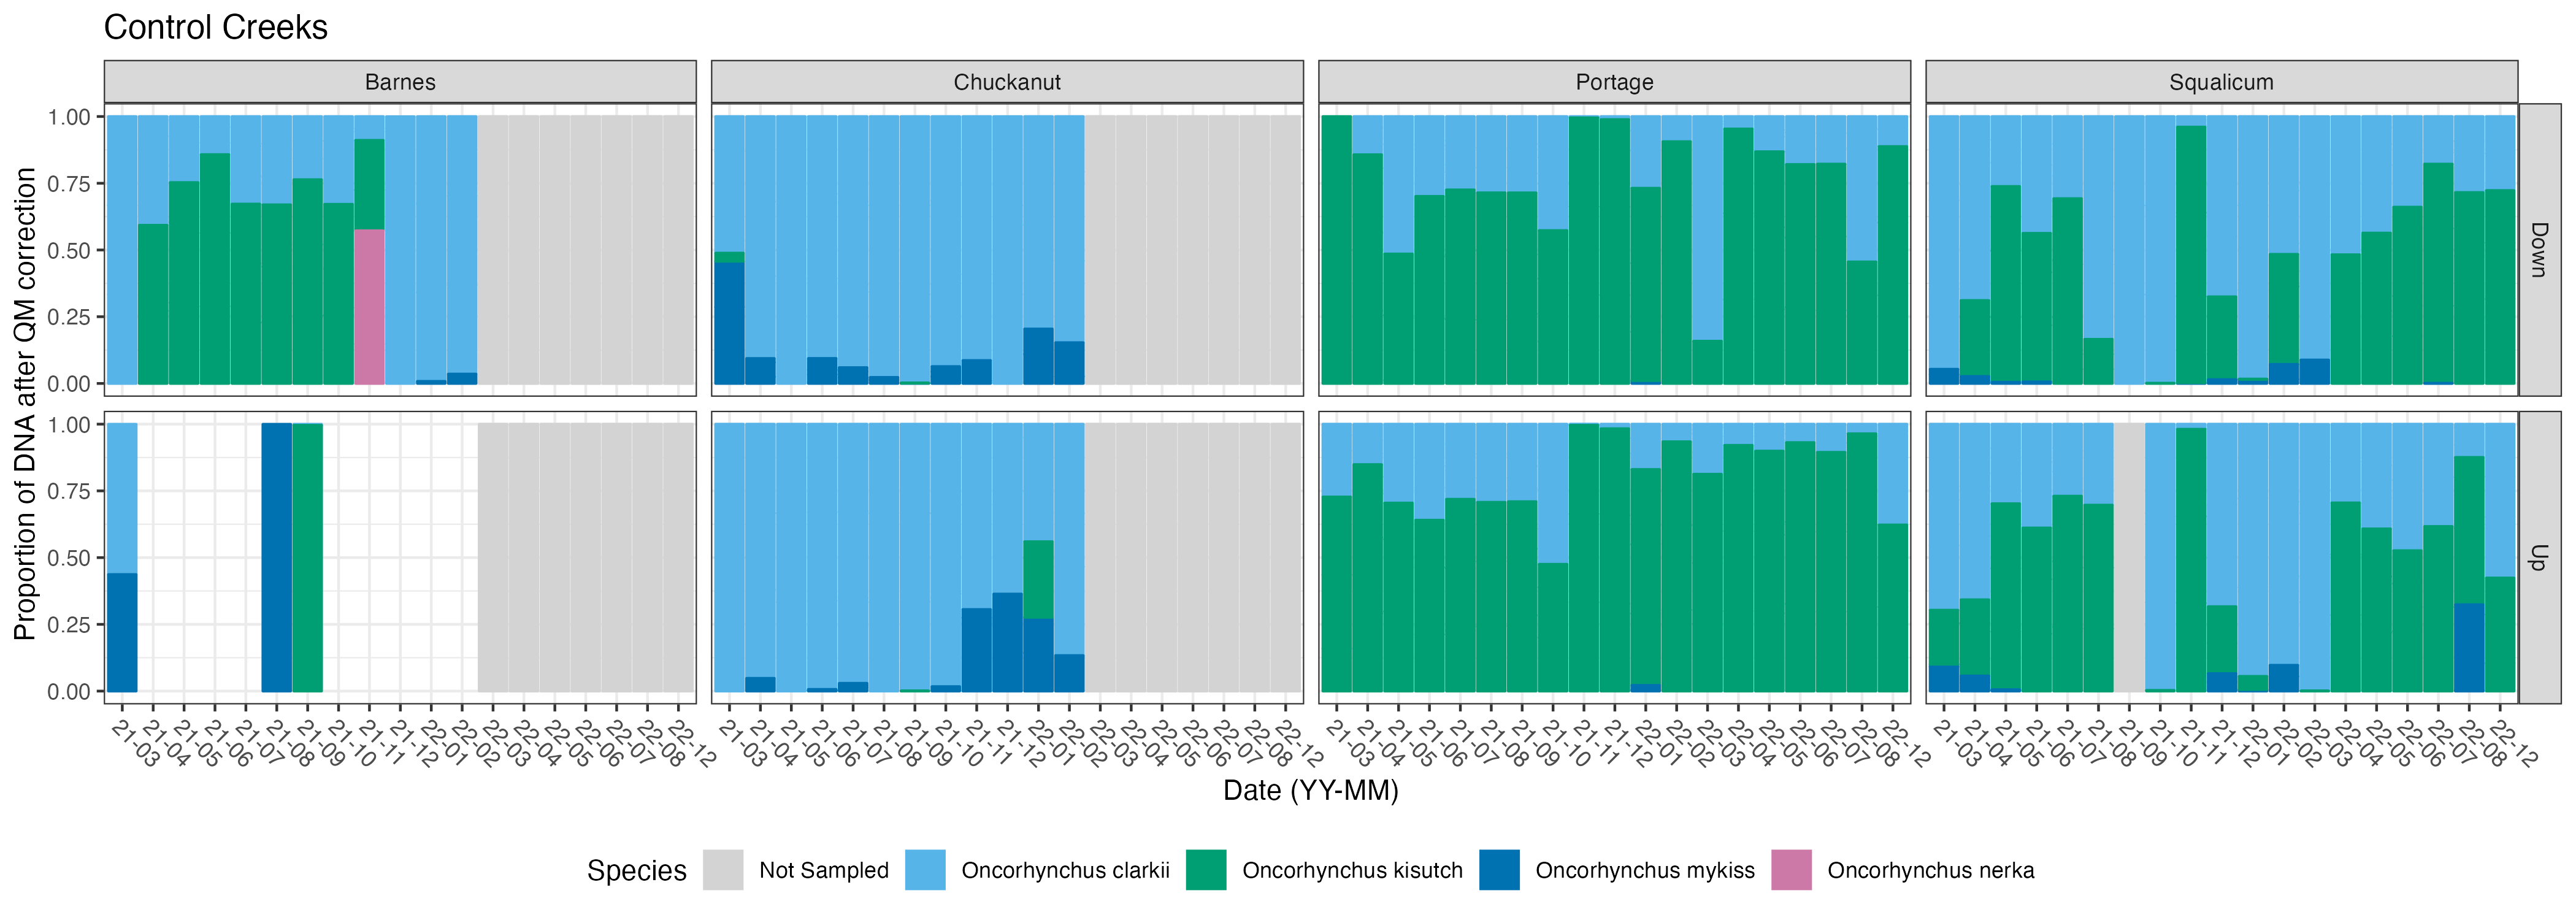
\includegraphics{../Output/Figures/proportions_after_qm_nopadden.png}
\DIFaddendFL \caption{Compositions of salmonid DNA \DIFaddbeginFL \DIFaddFL{in control creeks }\DIFaddendFL as determined by
metabarcoding after correction for amplification bias. \DIFdelbeginFL \DIFdelFL{Note }\DIFdelendFL \DIFaddbeginFL \DIFaddFL{Grey shading
denotes time points }\DIFaddendFL that \DIFdelbeginFL \DIFdelFL{no sampling occurred
}\DIFdelendFL \DIFaddbeginFL \DIFaddFL{were not sampled (Barnes and Chuckanut Creeks
after March 2023 and Squalicum Creek }\DIFaddendFL in September 2021 \DIFdelbeginFL \DIFdelFL{at Squalicum Creek because the creek }\DIFdelendFL \DIFaddbeginFL \DIFaddFL{which }\DIFaddendFL was dry\DIFaddbeginFL \DIFaddFL{)}\DIFaddendFL .
The empty bars in the Barnes upstream sites indicate that no salmonid
DNA was found at those time points.\DIFdelbeginFL %DIFDELCMD < \label{fig:qm}%%%
\DIFdelendFL \DIFaddbeginFL \label{fig:qm_controls}\DIFaddendFL }
\end{figure}

\DIFaddbegin \begin{figure}
\centering
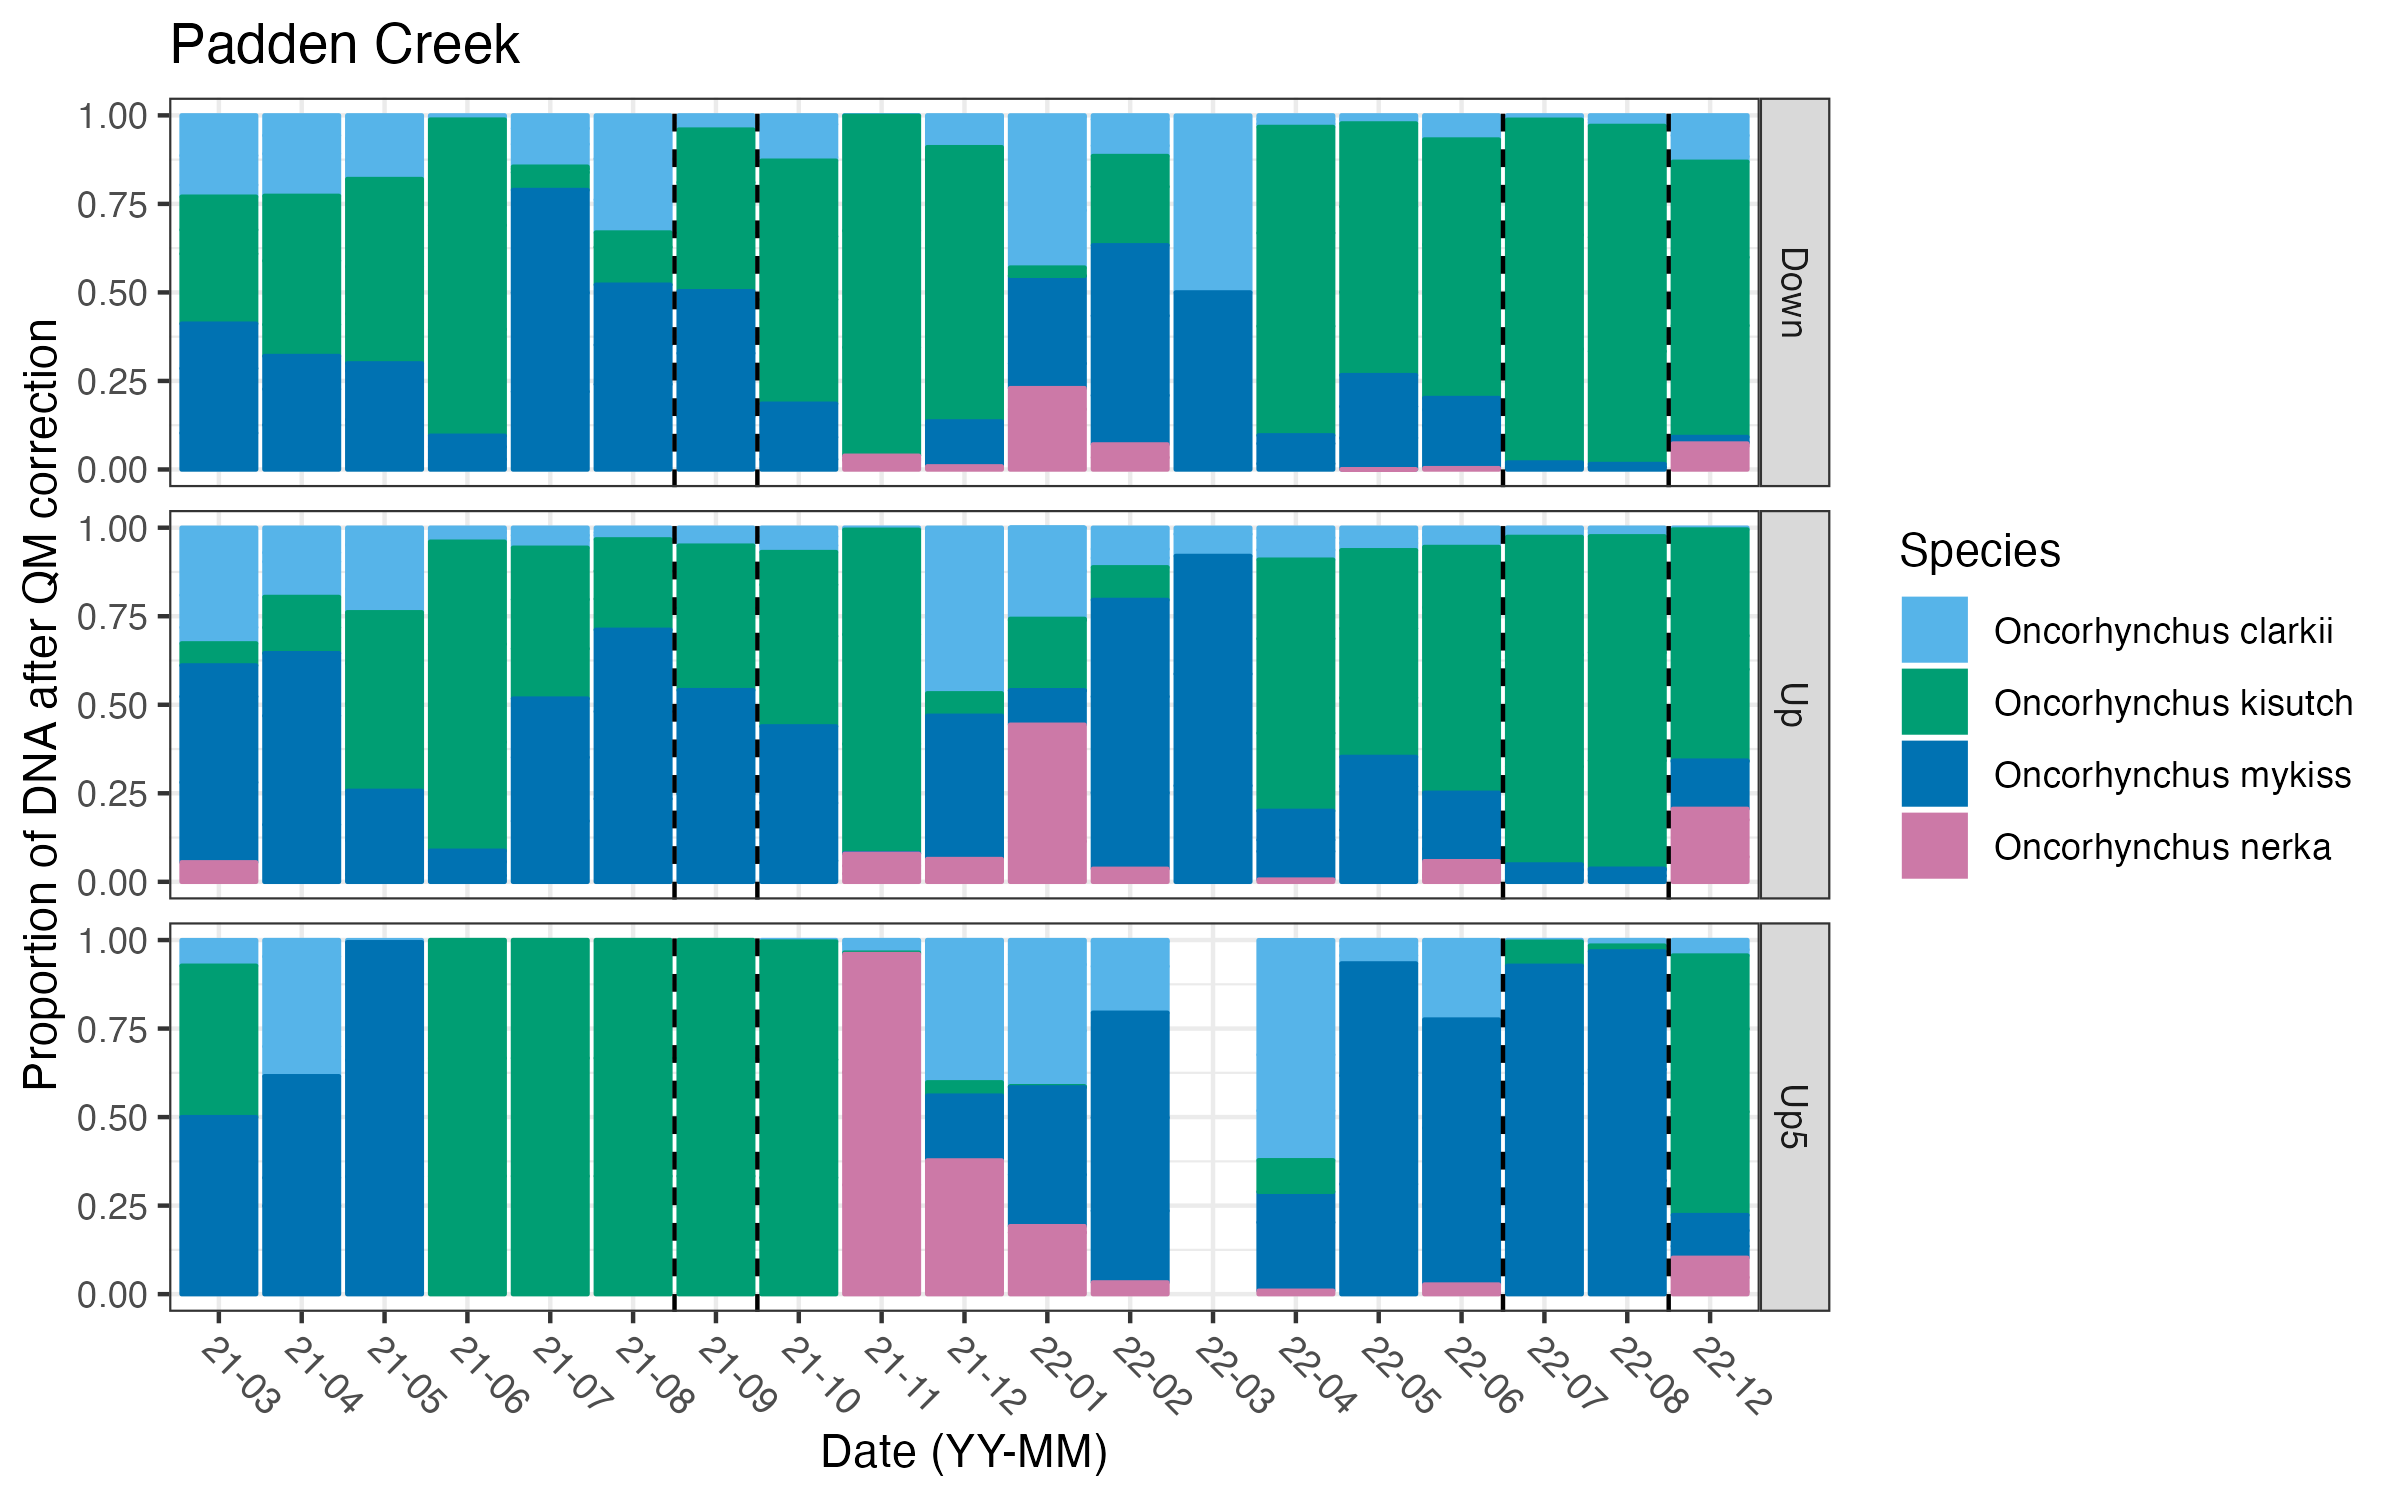
\includegraphics{../Output/Figures/proportions_after_qm_padden.png}
\caption{\DIFaddFL{Compositions of salmonid DNA in Padden Creek as determined by
metabarcoding after correction for amplification bias. The empty bar in
the March 2023 in Up5 indicates that no salmonid DNA was found. The
vertical dashed lines indicates the time period in which the culverts
were replaced (SR-11 and I-5, respectively).}\label{fig:qm_padden}}
\end{figure}

\DIFaddend All environmental samples were quantified for absolute concentrations of
cutthroat trout DNA across \DIFdelbegin \DIFdel{30 }\DIFdelend \DIFaddbegin \DIFadd{32 }\DIFaddend qPCR plates, resulting in
\DIFdelbegin \DIFdel{280 samples (\textasciitilde80}\DIFdelend \DIFaddbegin \DIFadd{\textasciitilde630 samples (\textasciitilde60}\DIFaddend \%) with a positive
detection in at least 1 of 3 technical replicates. The modeled output of
cutthroat trout DNA concentrations, ranged from \DIFdelbegin \DIFdel{10 }\DIFdelend \DIFaddbegin \DIFadd{50 }\DIFaddend copies/L to 1.4 x
10\textsuperscript{6} copies/L, with a mean value of
\DIFdelbegin \DIFdel{\textasciitilde58}\DIFdelend \DIFaddbegin \DIFadd{\textasciitilde47}\DIFaddend ,000 copies/L (Figure \ref{fig:qpcr}).

\begin{figure}
\centering
\DIFdelbeginFL %DIFDELCMD < \includegraphics{../Output/Figures/20230105_modeled_cut_qpcr_updown-line.png}
%DIFDELCMD < %%%
\DIFdelendFL \DIFaddbeginFL 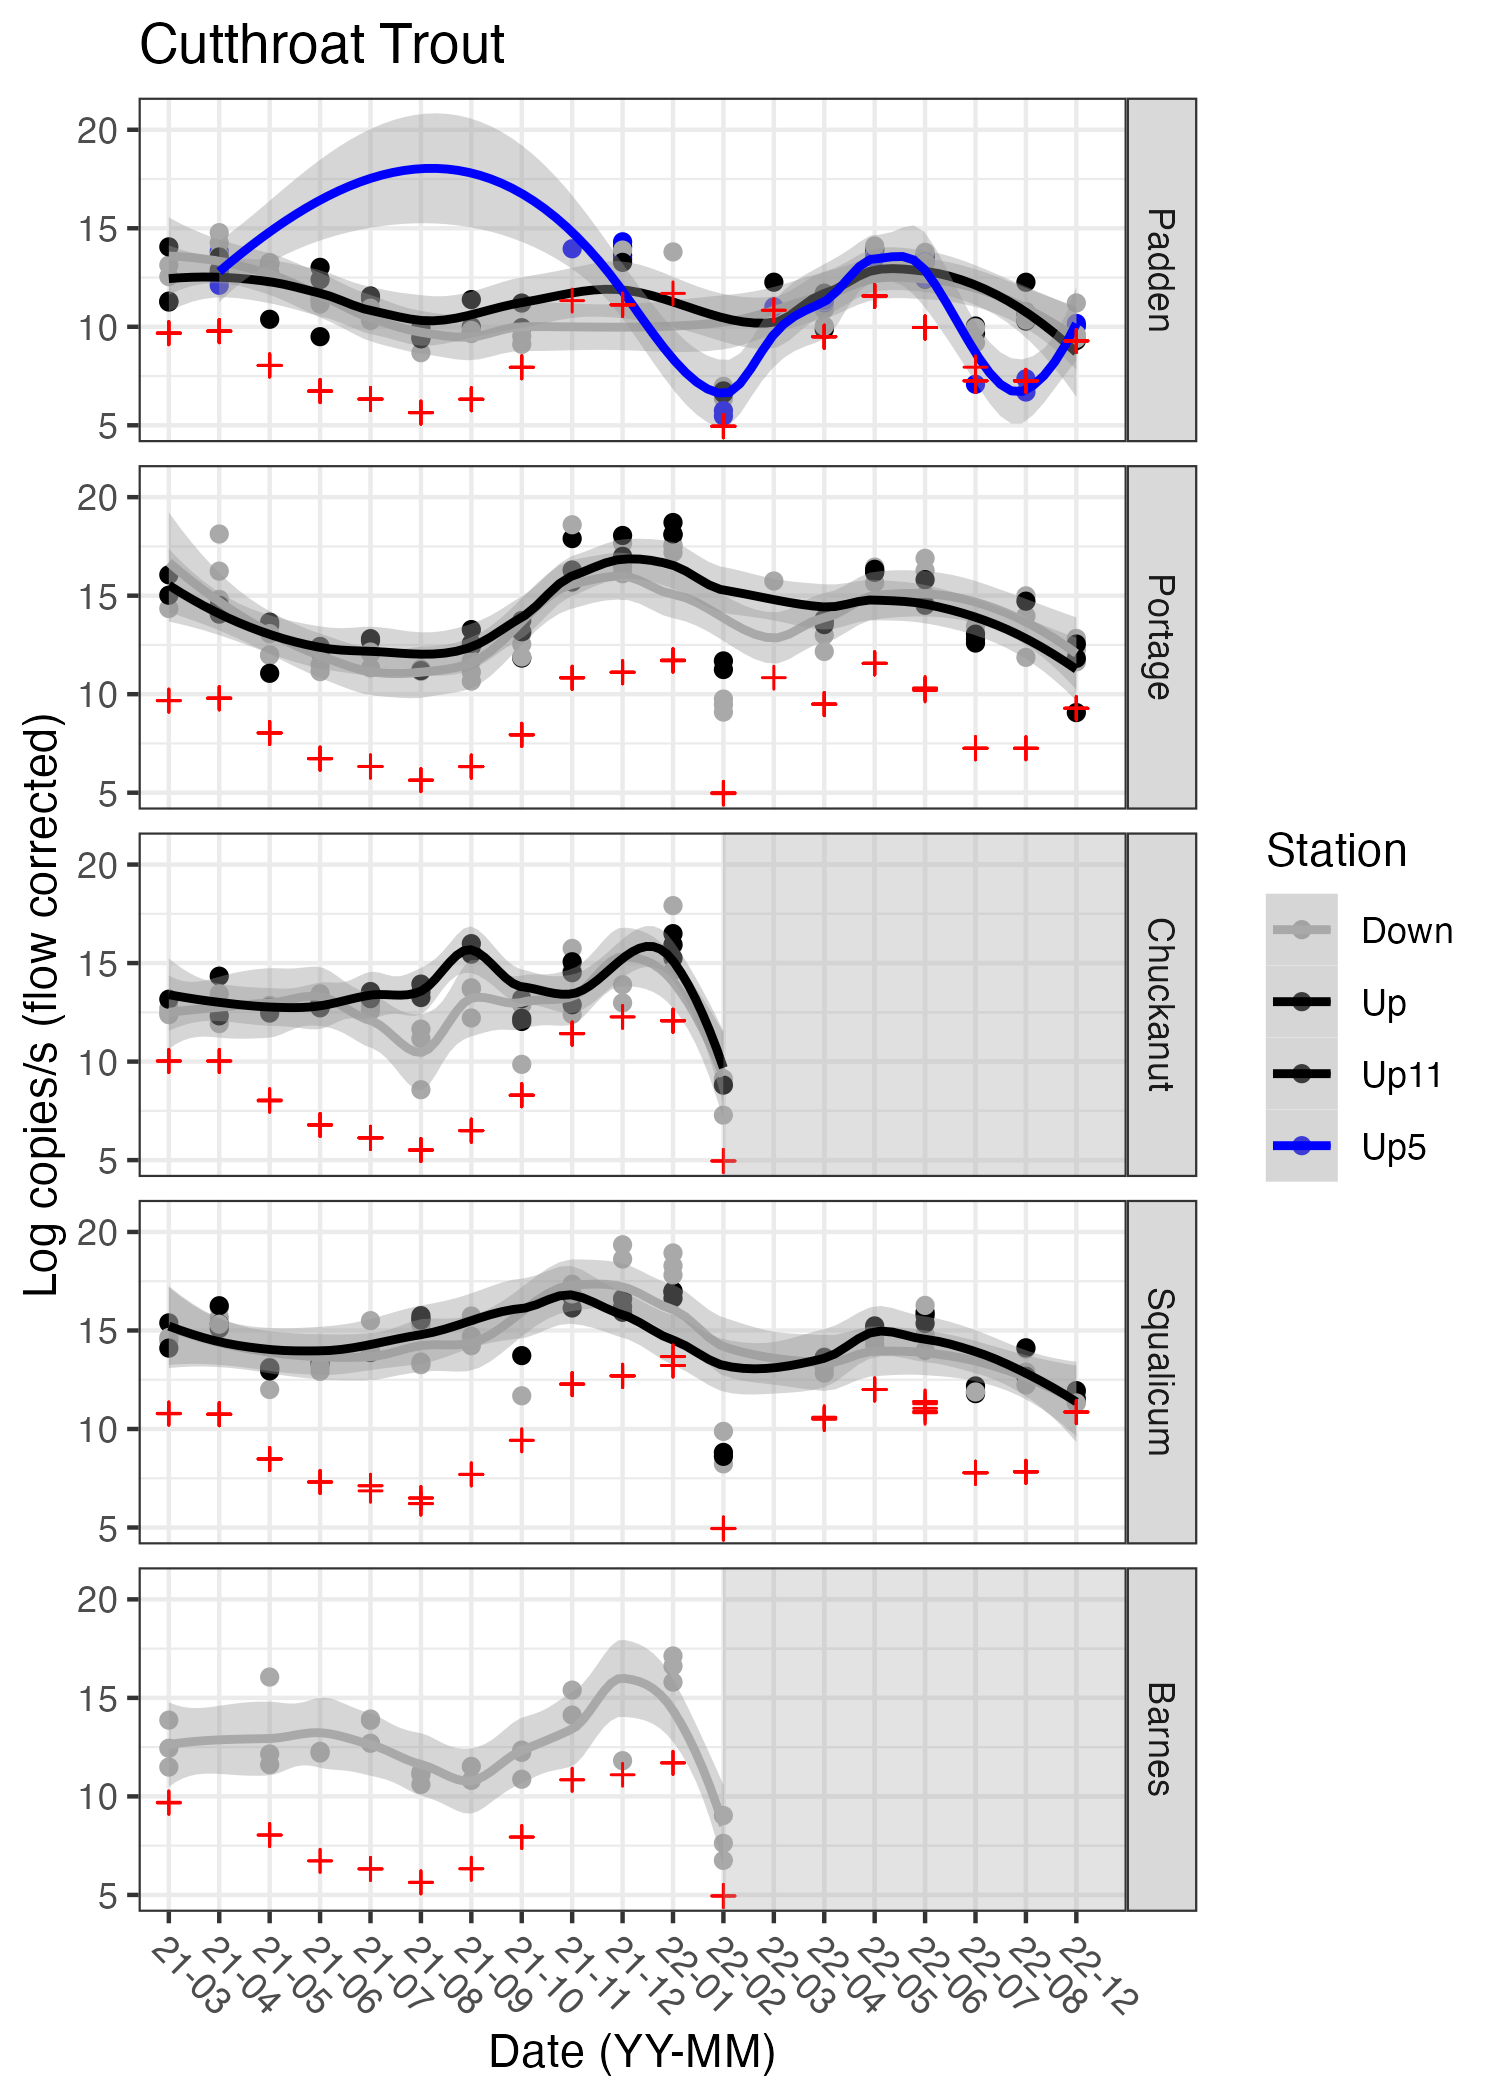
\includegraphics{../Output/Figures/modeled_cut_qpcr_updown_flowcorrected.png}
\DIFaddendFL \caption{Absolute \DIFdelbeginFL \DIFdelFL{concentration }\DIFdelendFL \DIFaddbeginFL \DIFaddFL{mass flow rate }\DIFaddendFL (log copies/\DIFdelbeginFL \DIFdelFL{L of water}\DIFdelendFL \DIFaddbeginFL \DIFaddFL{s}\DIFaddendFL ) of \DIFdelbeginFL \emph{\DIFdelFL{O.
clarkii}} %DIFAUXCMD
\DIFdelFL{(}\DIFdelendFL cutthroat trout
\DIFaddbeginFL \DIFaddFL{(}\emph{\DIFaddFL{O. clarkii}}\DIFaddendFL ) as measured by qPCR \DIFdelbeginFL \DIFdelFL{before }\DIFdelendFL \DIFaddbeginFL \DIFaddFL{after }\DIFaddendFL flow correction. \DIFaddbeginFL \DIFaddFL{Note that
Barnes Creek and Chuckanut Creek were not sampled after February 2022.
Red crosses show the limit of detection for each species and time point,
which changes with flow rate and total volume filtered per
sample.}\DIFaddendFL \label{fig:qpcr}}
\end{figure}

We combined compositional information from metabarcoding with absolute
concentrations \DIFaddbegin \DIFadd{from qPCR }\DIFaddend for our reference species, \DIFaddbegin \DIFadd{cutthroat trout
(}\DIFaddend \emph{O. clarkii}\DIFdelbegin \DIFdel{, from the
qPCR }\DIFdelend \DIFaddbegin \DIFadd{), }\DIFaddend to estimate the total concentration of DNA for each
species (See Supplemental Text 2). \DIFdelbegin \DIFdel{The joint time-series model shared information
across stations and creeks; consequently, data from one of the control
creeks (Barnes) could not be included because of the nearly total
absence of salmonids upstream of its culvert. However, data from the
remaining creeks characterized trends in the other }\DIFdelend \DIFaddbegin \DIFadd{These quantitative data for all }\DIFaddend four
target species \DIFdelbegin \DIFdel{well and could be modeled appropriately }\DIFdelend \DIFaddbegin \DIFadd{were then used in the linear mixed-effects model to
assess salmonid trends over time }\DIFaddend (Figure \ref{fig:ts}).

\begin{figure}
\centering
\DIFdelbeginFL %DIFDELCMD < \includegraphics{../Output/Figures/20221216_multispeciesTrends_flowcorrected.png}
%DIFDELCMD < %%%
\DIFdelendFL \DIFaddbeginFL 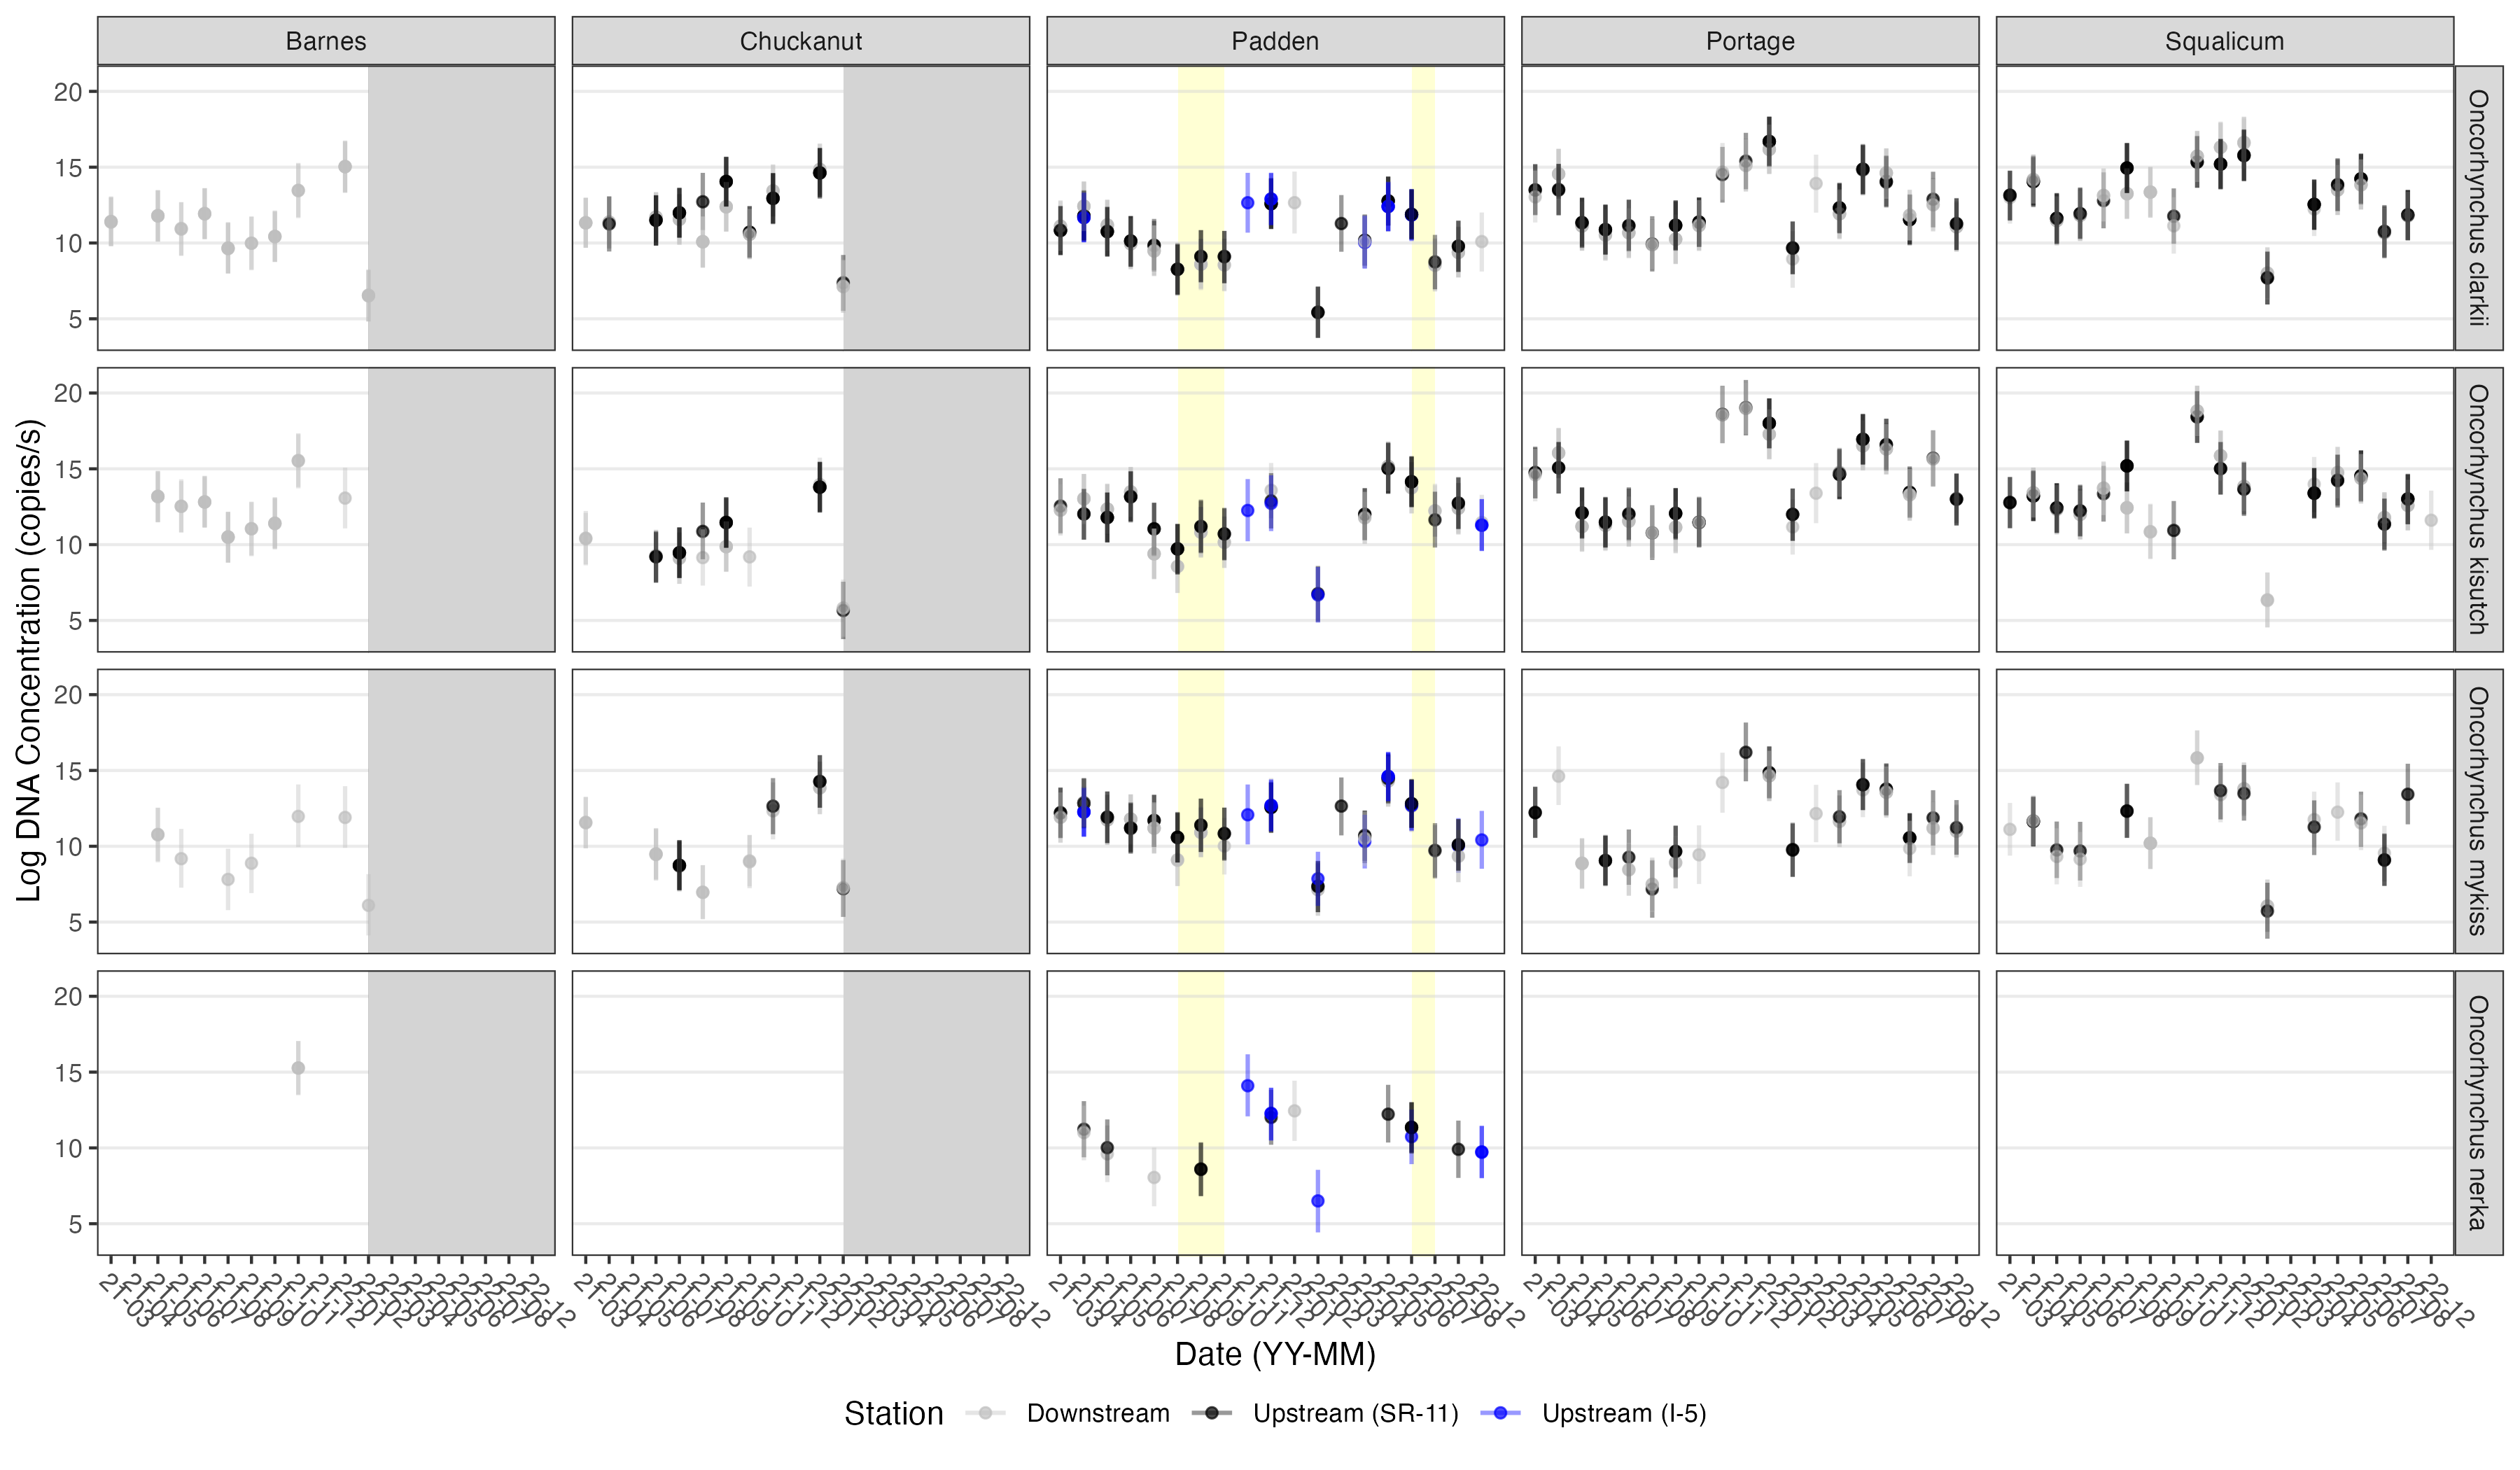
\includegraphics{../Output/Figures/multispeciesTrends_flowcorrected.png}
\DIFaddendFL \caption{Trends \DIFdelbeginFL \DIFdelFL{across creeks and across time }\DIFdelendFL \DIFaddbeginFL \DIFaddFL{in mass flow rate (log copies/s) }\DIFaddendFL for each of four
salmonid species \DIFaddbeginFL \DIFaddFL{across creeks and across time }\DIFaddendFL as estimated by eDNA
analysis. \DIFdelbeginFL \DIFdelFL{Light-colored dots are }\DIFdelendFL \DIFaddbeginFL \DIFaddFL{Points represent }\DIFaddendFL posterior means \DIFdelbeginFL \DIFdelFL{derived by expanding the calibrated metabarcoding proportions as
described in the main text; darker-colored dots are posterior means }\DIFdelendFL for the \DIFdelbeginFL \DIFdelFL{time-series }\DIFdelendFL \DIFaddbeginFL \DIFaddFL{linear mixed effects
}\DIFaddendFL model \DIFdelbeginFL \DIFdelFL{of }\DIFdelendFL \DIFaddbeginFL \DIFaddFL{and error bars represent }\DIFaddendFL the \DIFdelbeginFL \DIFdelFL{same}\DIFdelendFL \DIFaddbeginFL \DIFaddFL{95\% posterior confidence interval}\DIFaddendFL .
Colors indicate station upstream \DIFaddbeginFL \DIFaddFL{(black) }\DIFaddendFL or downstream \DIFaddbeginFL \DIFaddFL{(grey) }\DIFaddendFL of \DIFaddbeginFL \DIFaddFL{the
culvert. Padden has }\DIFaddendFL an \DIFdelbeginFL \DIFdelFL{under-road }\DIFdelendFL \DIFaddbeginFL \DIFaddFL{additional sampling site upstream of the second
}\DIFaddendFL culvert \DIFaddbeginFL \DIFaddFL{(I-5; blue)}\DIFaddendFL . \DIFdelbeginFL \DIFdelFL{75\% and 95\% posterior CI plotted
for each time point. Grey }\DIFdelendFL \DIFaddbeginFL \DIFaddFL{Yellow }\DIFaddendFL shading indicates the time period in which
the \DIFdelbeginFL \DIFdelFL{culvert }\DIFdelendFL \DIFaddbeginFL \DIFaddFL{culverts }\DIFaddendFL in the treatment creek (Padden Creek) \DIFdelbeginFL \DIFdelFL{was
}\DIFdelendFL \DIFaddbeginFL \DIFaddFL{were }\DIFaddendFL replaced. \DIFaddbeginFL \DIFaddFL{Grey
shading indicates time points that were not sampled (Barnes and
Chuckanut after February 2022). Time points with no data had no
sequencing reads corresponding to that species or no quantifiable
cutthroat DNA by qPCR.}\DIFaddendFL \label{fig:ts}}

\end{figure}

\hypertarget{effects-of-culverts}{%
\subsubsection{Effects of Culverts}\label{effects-of-culverts}}

Before considering the effect of construction, the difference in \DIFdelbegin \DIFdel{abundance }\DIFdelend trends
between upstream and downstream stations (Figure \ref{fig:ts})
demonstrates that the culverts themselves have some effect, but
\DIFaddbegin \DIFadd{generally }\DIFaddend not a large effect on the salmonid species surveyed. \DIFdelbegin \DIFdel{Therefore, these four creeks (which include 3 culverts and one bridge)
do not seem to be blocking salmonid passage, A noteable }\DIFdelend \DIFaddbegin \DIFadd{A notable
}\DIFaddend exception was Barnes Creek, \DIFdelbegin \DIFdel{which was not included in the time series model, }\DIFdelend as the culvert was so clearly a barrier as
most time points had no salmonid DNA upstream\DIFdelbegin \DIFdel{and therefore models including Barnes do not converge as a result of the large fraction of sampling points with no observations of
salmonids.
(Figure \ref{fig:qm}).
}\DIFdelend \DIFaddbegin \DIFadd{. Padden Creek upstream of
I-5 also was more clearly a barrier to fish passage, while the culvert
across SR-11 seemed to be less of a barrier to fish passage. In other
cases, salmonid DNA is found upstream but not downstream, indicating
that the culvert is likely not a barrier and there are resident
individuals upstream of the culvert.
}\DIFaddend 

Summarizing over all species and the four creeks used in the time series
model, the \DIFdelbegin \DIFdel{effect was largest during the dry periods of late summer /
early fall (July to October), when flows were at a minimum (i.e.,
September) and the
connectivity }\DIFdelend \DIFaddbegin \DIFadd{culvert effect was minimal (Figure \ref{fig:culverts}); the
average log-fold change }\DIFaddend between upstream and downstream \DIFdelbegin \DIFdel{was low
(Figure \ref{fig:culverts}). Salmonid species DNA concentrations were
higher upstream than downstream during this period, with mean upstream
DNA concentrations only about 5\% higher than downstream DNA
concentrations. }\DIFdelend \DIFaddbegin \DIFadd{sites was not
significantly different from zero. }\DIFaddend Individual species' patterns were
similar, indicating that there is not a species-specific effect where
culverts block the passage of some salmon but not others (\DIFdelbegin \DIFdel{Supplemental Figure 17).
A
notable exception is }\emph{\DIFdel{O. kisutch}} %DIFAUXCMD
\DIFdel{in Chuckanut Creek , which was
overall much more variable where salmonid DNA concentrations were up to
30\% higher upstream than downstream at certain time points and up to
44\% higher downstream and upstream at others. Across all species}\DIFdelend \DIFaddbegin \DIFadd{Figure S1.12).
The maximum positive log-fold change (i.e., upstream having a higher
mass flow rate) was 2.78 in Squalicum Creek for coho salmon (}\emph{\DIFadd{O.
kisutch}}\DIFadd{) in August 2021, while the maximum negative log-fold change
(i.e., downstream having a higher mass flow rate) was -1.11 found in
Squalicum Creek for cutthroat trout (}\emph{\DIFadd{O. clarkii}}\DIFadd{) in December 2021
(Figure S1.12). Of all species, creeks, }\DIFaddend and time points, \DIFdelbegin \DIFdel{Squalicum Creek had the lowest mean percent difference in
upstream and downstreamsalmonid DNA concentrations}\DIFdelend \DIFaddbegin \DIFadd{23 of the 151
observations were within a log-fold change of -0.1 to 0.1, which
corresponds with eDNA mass flow rates upstream within 10\% of mass flow
rates downstream}\DIFaddend .

\begin{figure}
\centering
\DIFdelbeginFL %DIFDELCMD < \includegraphics{../Output/Figures/20221216_culvert_effect_flowcorrected.png}
%DIFDELCMD < %%%
\DIFdelendFL \DIFaddbeginFL 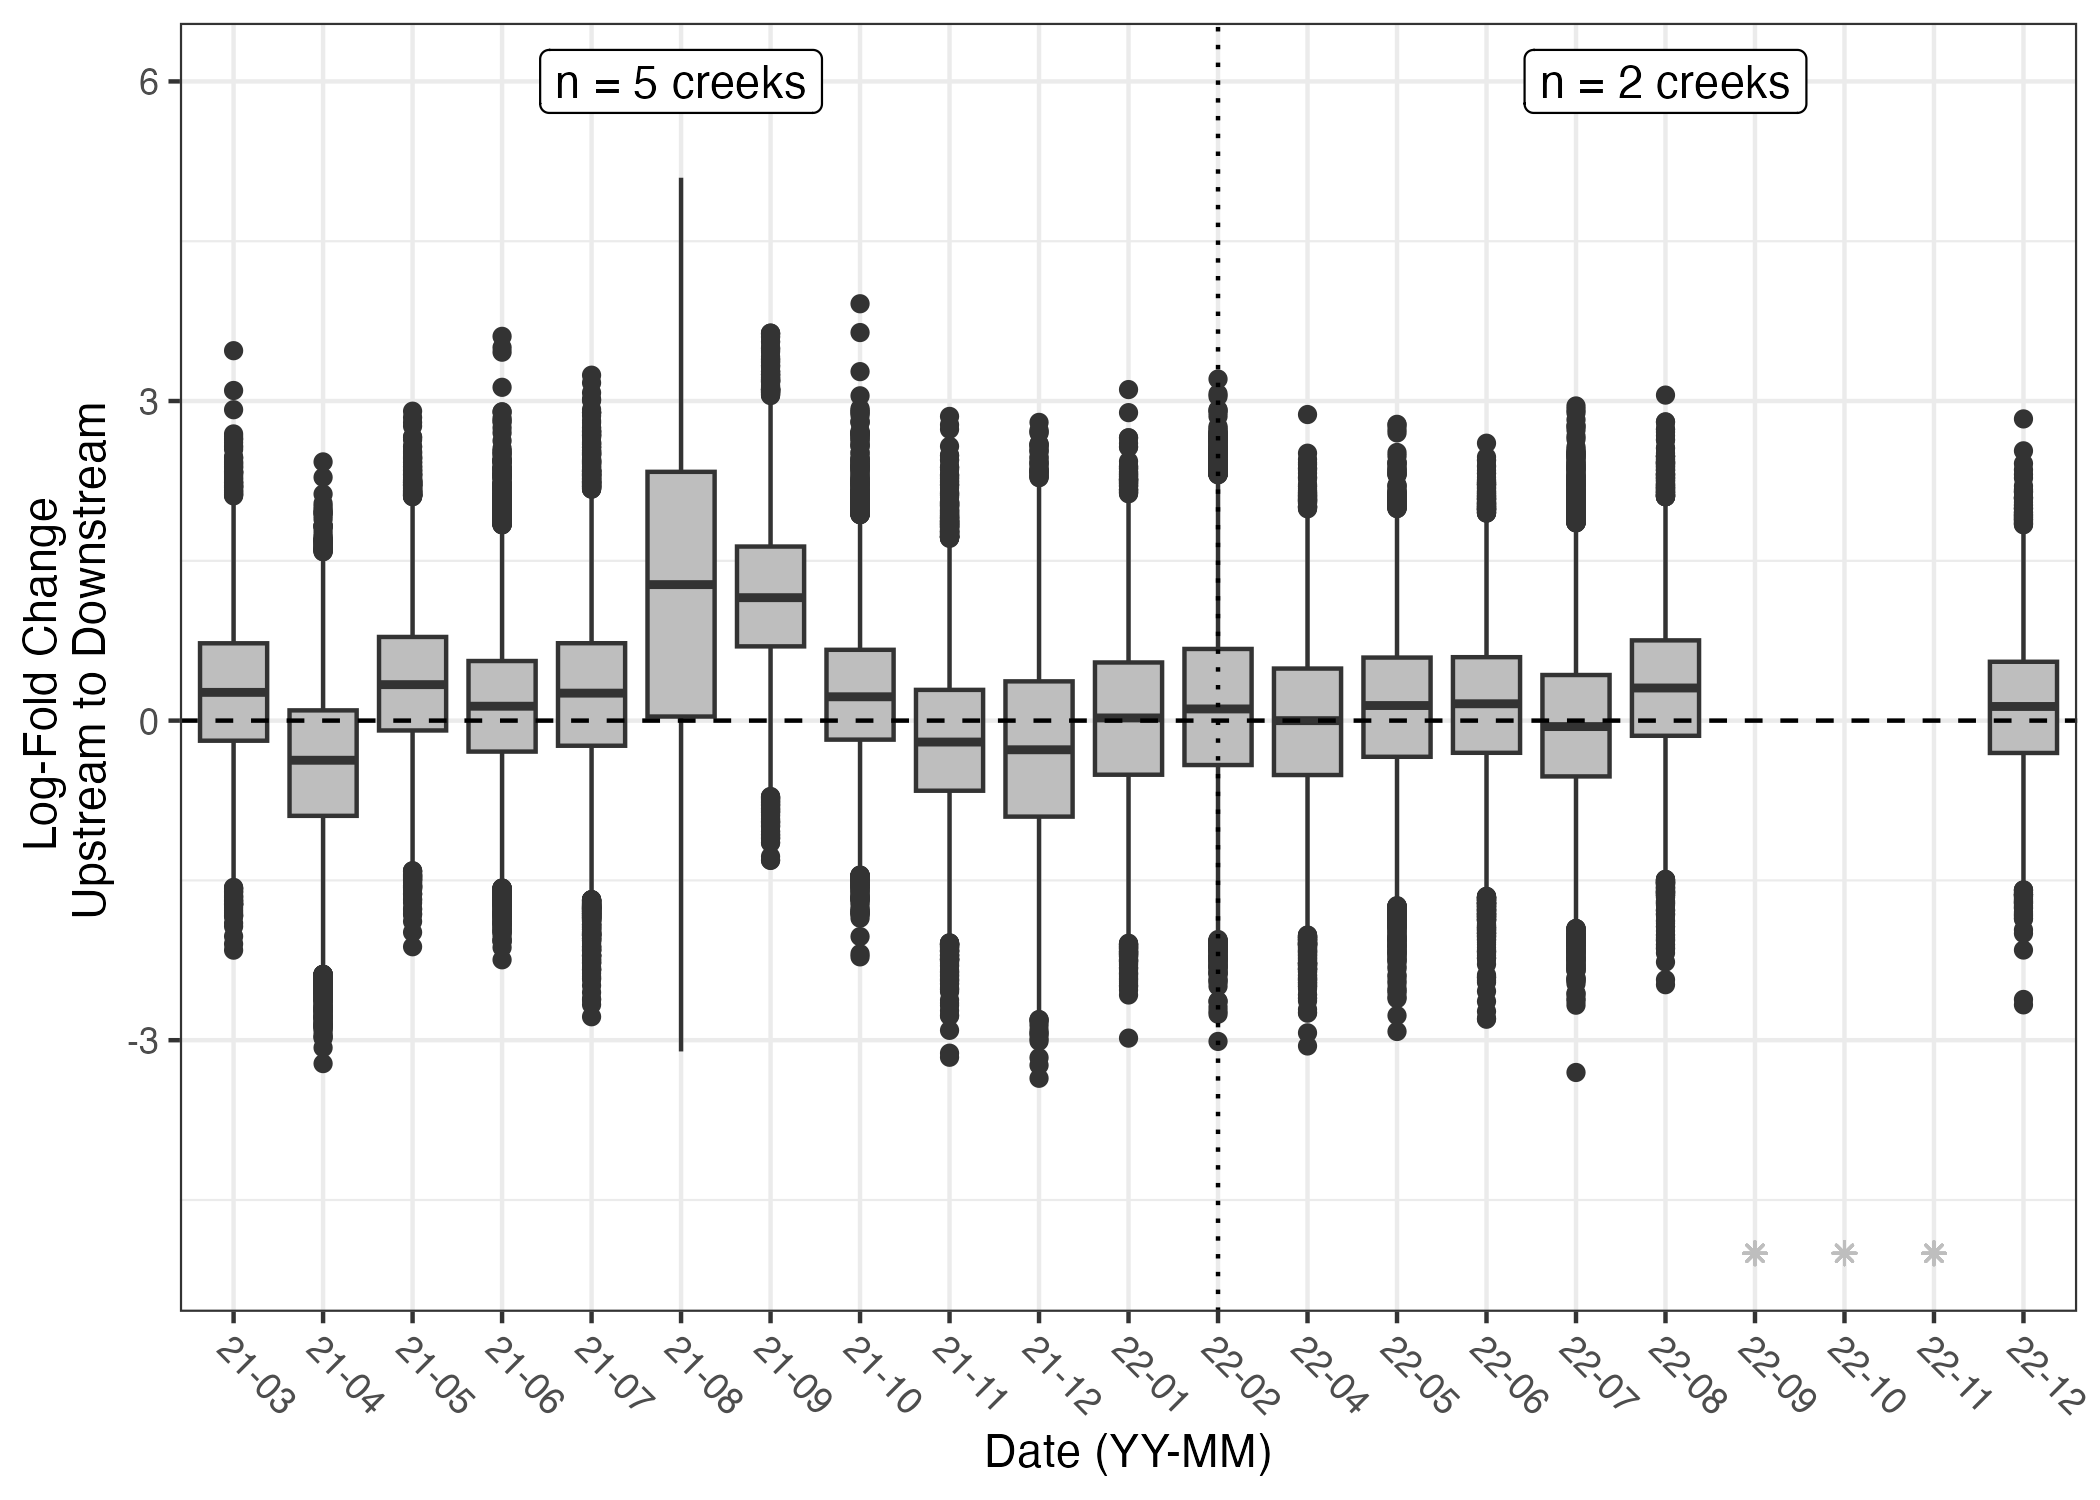
\includegraphics{../Output/Figures/culvert_boxplot_passable.png}
\DIFaddendFL \caption{The effect of culvert on salmonid abundance summed across all
species and creeks by time. The y-axis shows the \DIFdelbeginFL \DIFdelFL{difference }\DIFdelendFL \DIFaddbeginFL \DIFaddFL{log-fold change in eDNA
mass flow rate (copies/s) }\DIFaddendFL between upstream and downstream\DIFdelbeginFL \DIFdelFL{concentrations}\DIFdelendFL , normalized by
\DIFdelbeginFL \DIFdelFL{downstream
concentration}\DIFdelendFL \DIFaddbeginFL \DIFaddFL{upstream mass flow rate}\DIFaddendFL . The box boundaries correspond to the 25th and
75th percentiles; the whiskers correspond to 1.5 times the interquartile
range. Here, negative values imply that eDNA \DIFdelbeginFL \DIFdelFL{concentrations }\DIFdelendFL \DIFaddbeginFL \DIFaddFL{mass flow rates }\DIFaddendFL are higher
downstream than upstream. \DIFaddbeginFL \DIFaddFL{Samples with very low eDNA mass flow rates
(\textless{} 150 copies/s) were removed before plotting to remove
extreme proportional values due to large denominators. Grey stars
indicate times when no samples were taken.}\DIFaddendFL \label{fig:culverts}}
\end{figure}

\DIFaddbegin \DIFadd{We also considered how the log-fold change in eDNA mass flow rates were
impacted by the flow rate or discharge of the creek itself (Figure
\ref{fig:culverts_flow}. We found that at months of the lowest flow
(summer months), the log-fold changes between mass flow rates were the
highest, while in winter months with highest discharge the log-fold
changes were lower and downstream sites often had higher eDNA mass flow
rates than upstream sites (Figure S1.12).
}
\begin{figure}
\centering
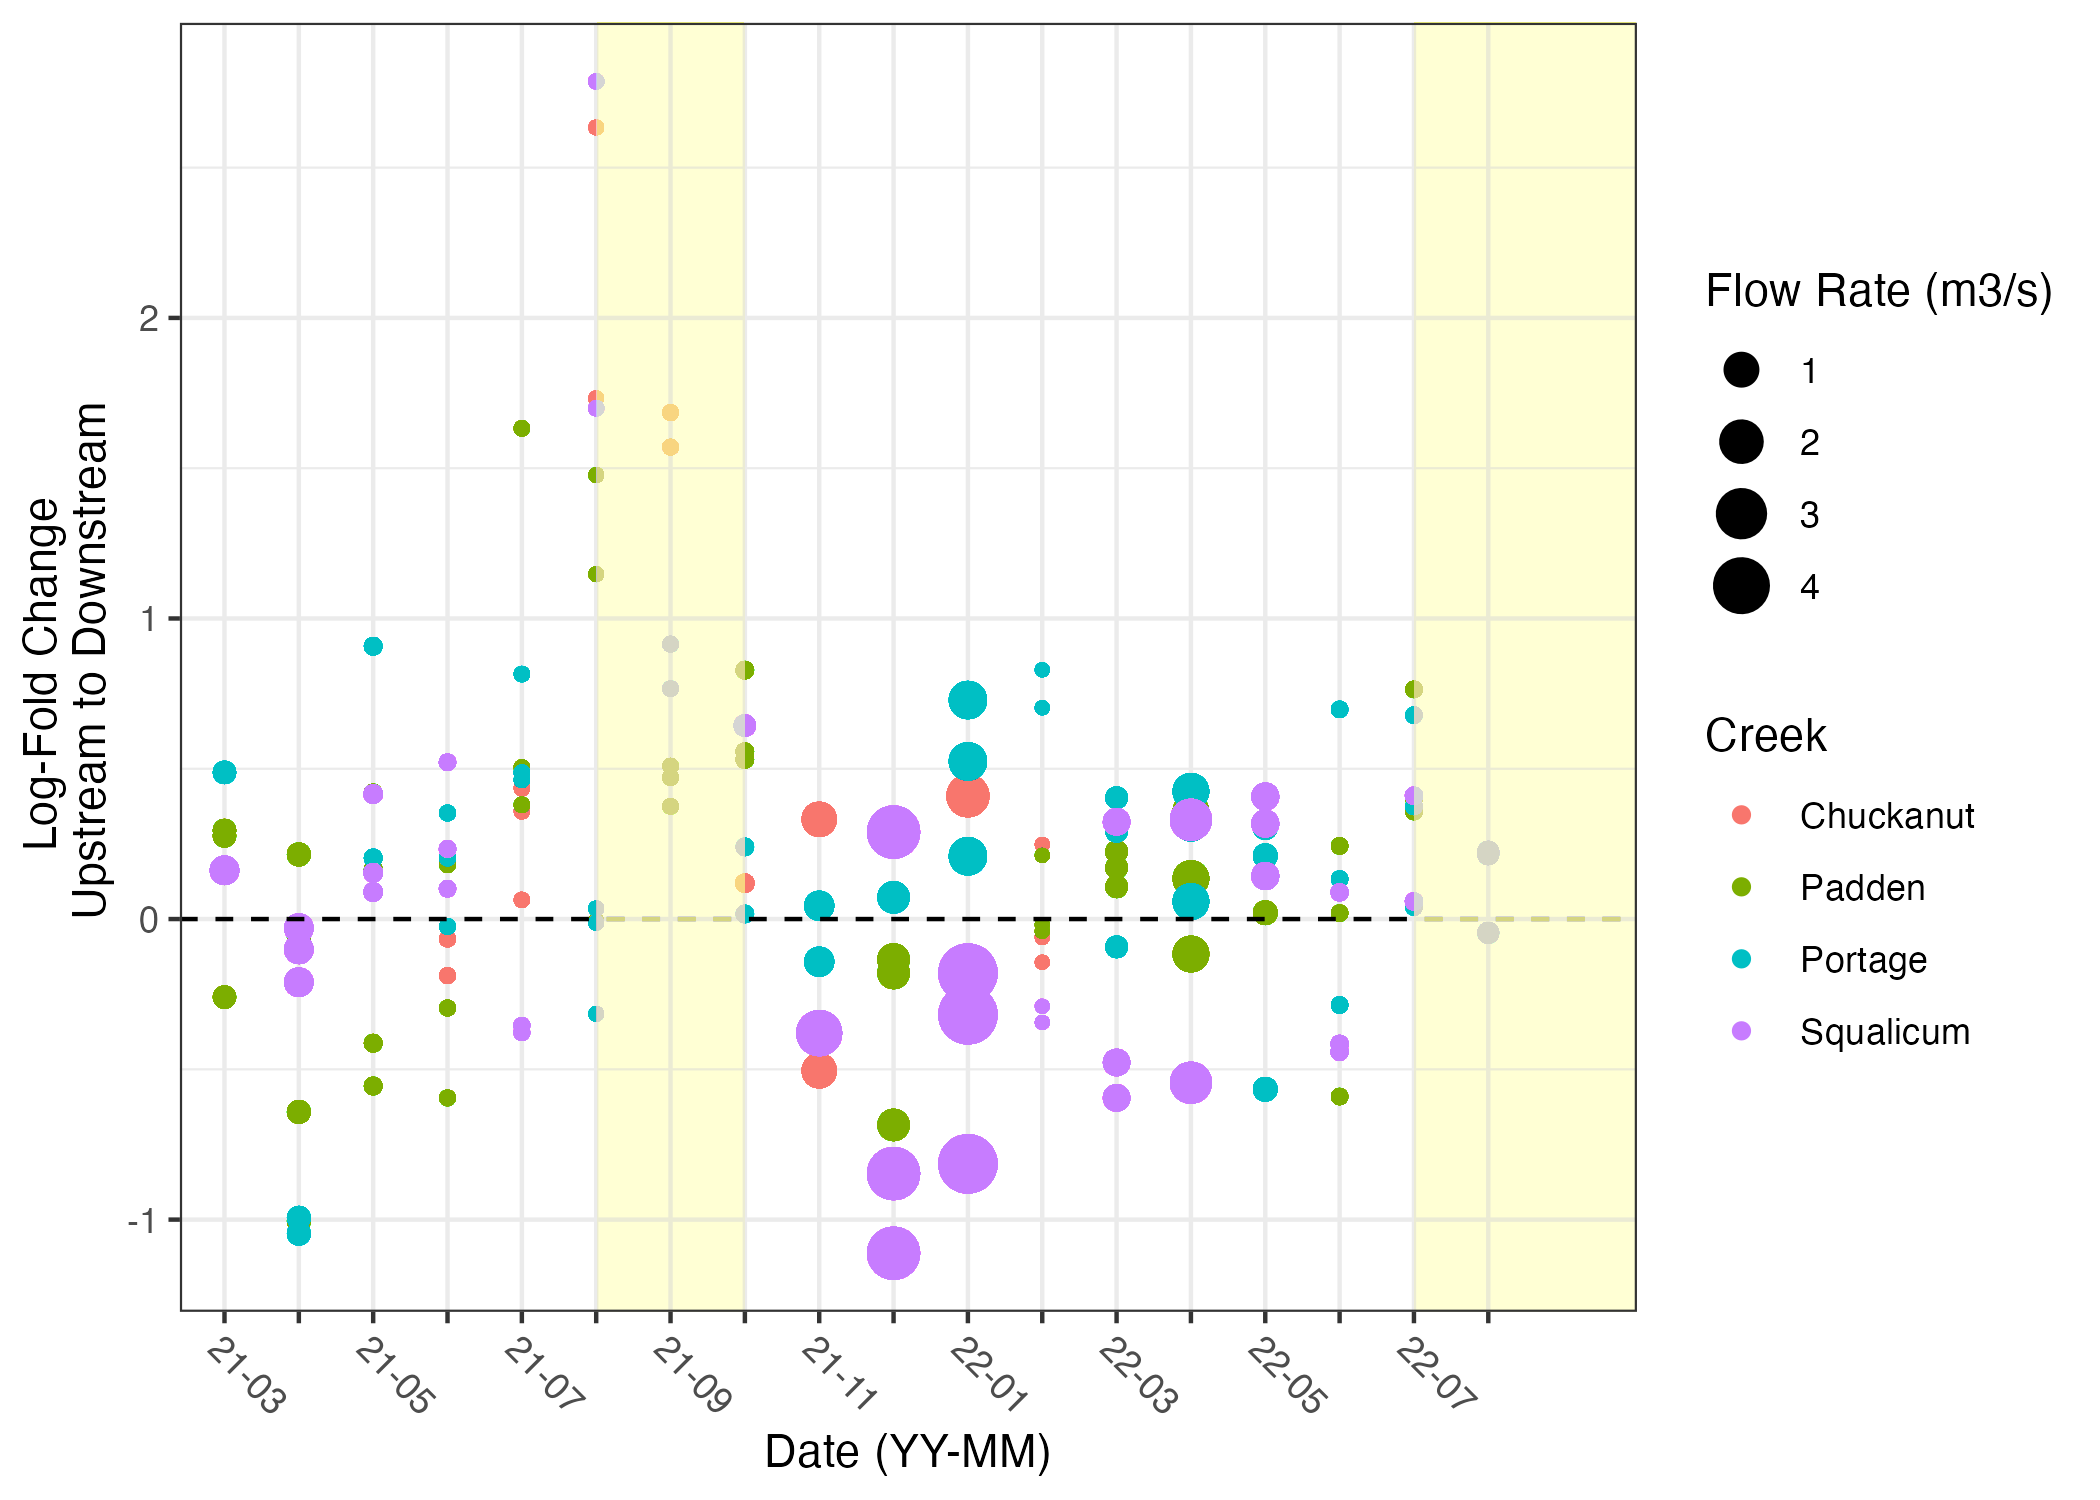
\includegraphics{../Output/Figures/culvert_means_flow.png}
\caption{\DIFaddFL{Log-fold change in eDNA mass flow rate over time. Size of
circles corresponds to the discharge in each creek at each time point.
Color of circles corresponds to each creek. Each creek and time point
has up to four circles of the same color for the four salmonid
species.}\label{fig:culverts_flow}}

\end{figure}

\DIFaddend \hypertarget{effects-of-culvert-replacement}{%
\subsubsection{Effects of Culvert
Replacement}\label{effects-of-culvert-replacement}}

\DIFdelbegin \DIFdel{Fish were excluded from Padden Creek on August 30th, 2021 in preparation
for the stream to be diverted on September 9th, 2021 and the diversion
was removed October 7th, 2021. Water sampling occurred on September
10th, 2021, the day after the
diversion, and on October 12, 2021, just 5
days after reconnecting the stream (Supplemental Figure 3).
}\DIFdelend By comparing the difference in upstream and downstream \DIFdelbegin \DIFdel{concentrations }\DIFdelend \DIFaddbegin \DIFadd{mass flow rates
}\DIFaddend before and after construction in Padden Creek, we can assess how large
of an impact the \DIFdelbegin \DIFdel{replacement }\DIFdelend \DIFaddbegin \DIFadd{two culvert replacements }\DIFaddend had on salmonid species
\DIFdelbegin \DIFdel{.
}%DIFDELCMD < 

%DIFDELCMD < %%%
\DIFdelend \DIFaddbegin \DIFadd{(Figure \ref{fig:construction}). }\DIFaddend The effects of the culvert replacement
\DIFdelbegin \DIFdel{operation }\DIFdelend \DIFaddbegin \DIFadd{operations }\DIFaddend appeared to have been transient and fairly minor for the four
salmonid species surveyed. \DIFdelbegin \DIFdel{After
the beginning of construction in September 2021 through the end of
sampling in February 2022, we }\DIFdelend \DIFaddbegin \DIFadd{We }\DIFaddend saw very minor fluctuations in the
difference between upstream and downstream salmonid DNA \DIFdelbegin \DIFdel{concentrations}\DIFdelend \DIFaddbegin \DIFadd{mass flow rates}\DIFaddend ,
and did not see an increase in this difference due to the culvert
removal \DIFaddbegin \DIFadd{as the log-fold changes in Padden Creek were similar to those in
the control creeks at the same time points }\DIFaddend (Figure
\ref{fig:construction}, grey \DIFdelbegin \DIFdel{shading }\DIFdelend \DIFaddbegin \DIFadd{points }\DIFaddend vs.~\DIFdelbegin \DIFdel{no shading).
Overall, }\emph{\DIFdel{O. clarkii}} %DIFAUXCMD
\DIFdel{was the least impacted species of the
construction while }\emph{\DIFdel{O. nerka}} %DIFAUXCMD
\DIFdel{was the most impacted species, likely
due to the very low concentrations in the creek and the migration timing
of }\emph{\DIFdel{O. nerka}} %DIFAUXCMD
\DIFdel{being during and post-restoration. The mean percent
difference across all species prior to construction was 0.18\% compared
to 1.6\% during and post-construction (Supplemental Table 2}\DIFdelend \DIFaddbegin \DIFadd{black points in areas of yellow
shading}\DIFaddend ).

\begin{figure}
\centering
\DIFdelbeginFL %DIFDELCMD < \includegraphics{../Output/Figures/20221219_construction_plot.png}
%DIFDELCMD < %%%
\DIFdelendFL \DIFaddbeginFL 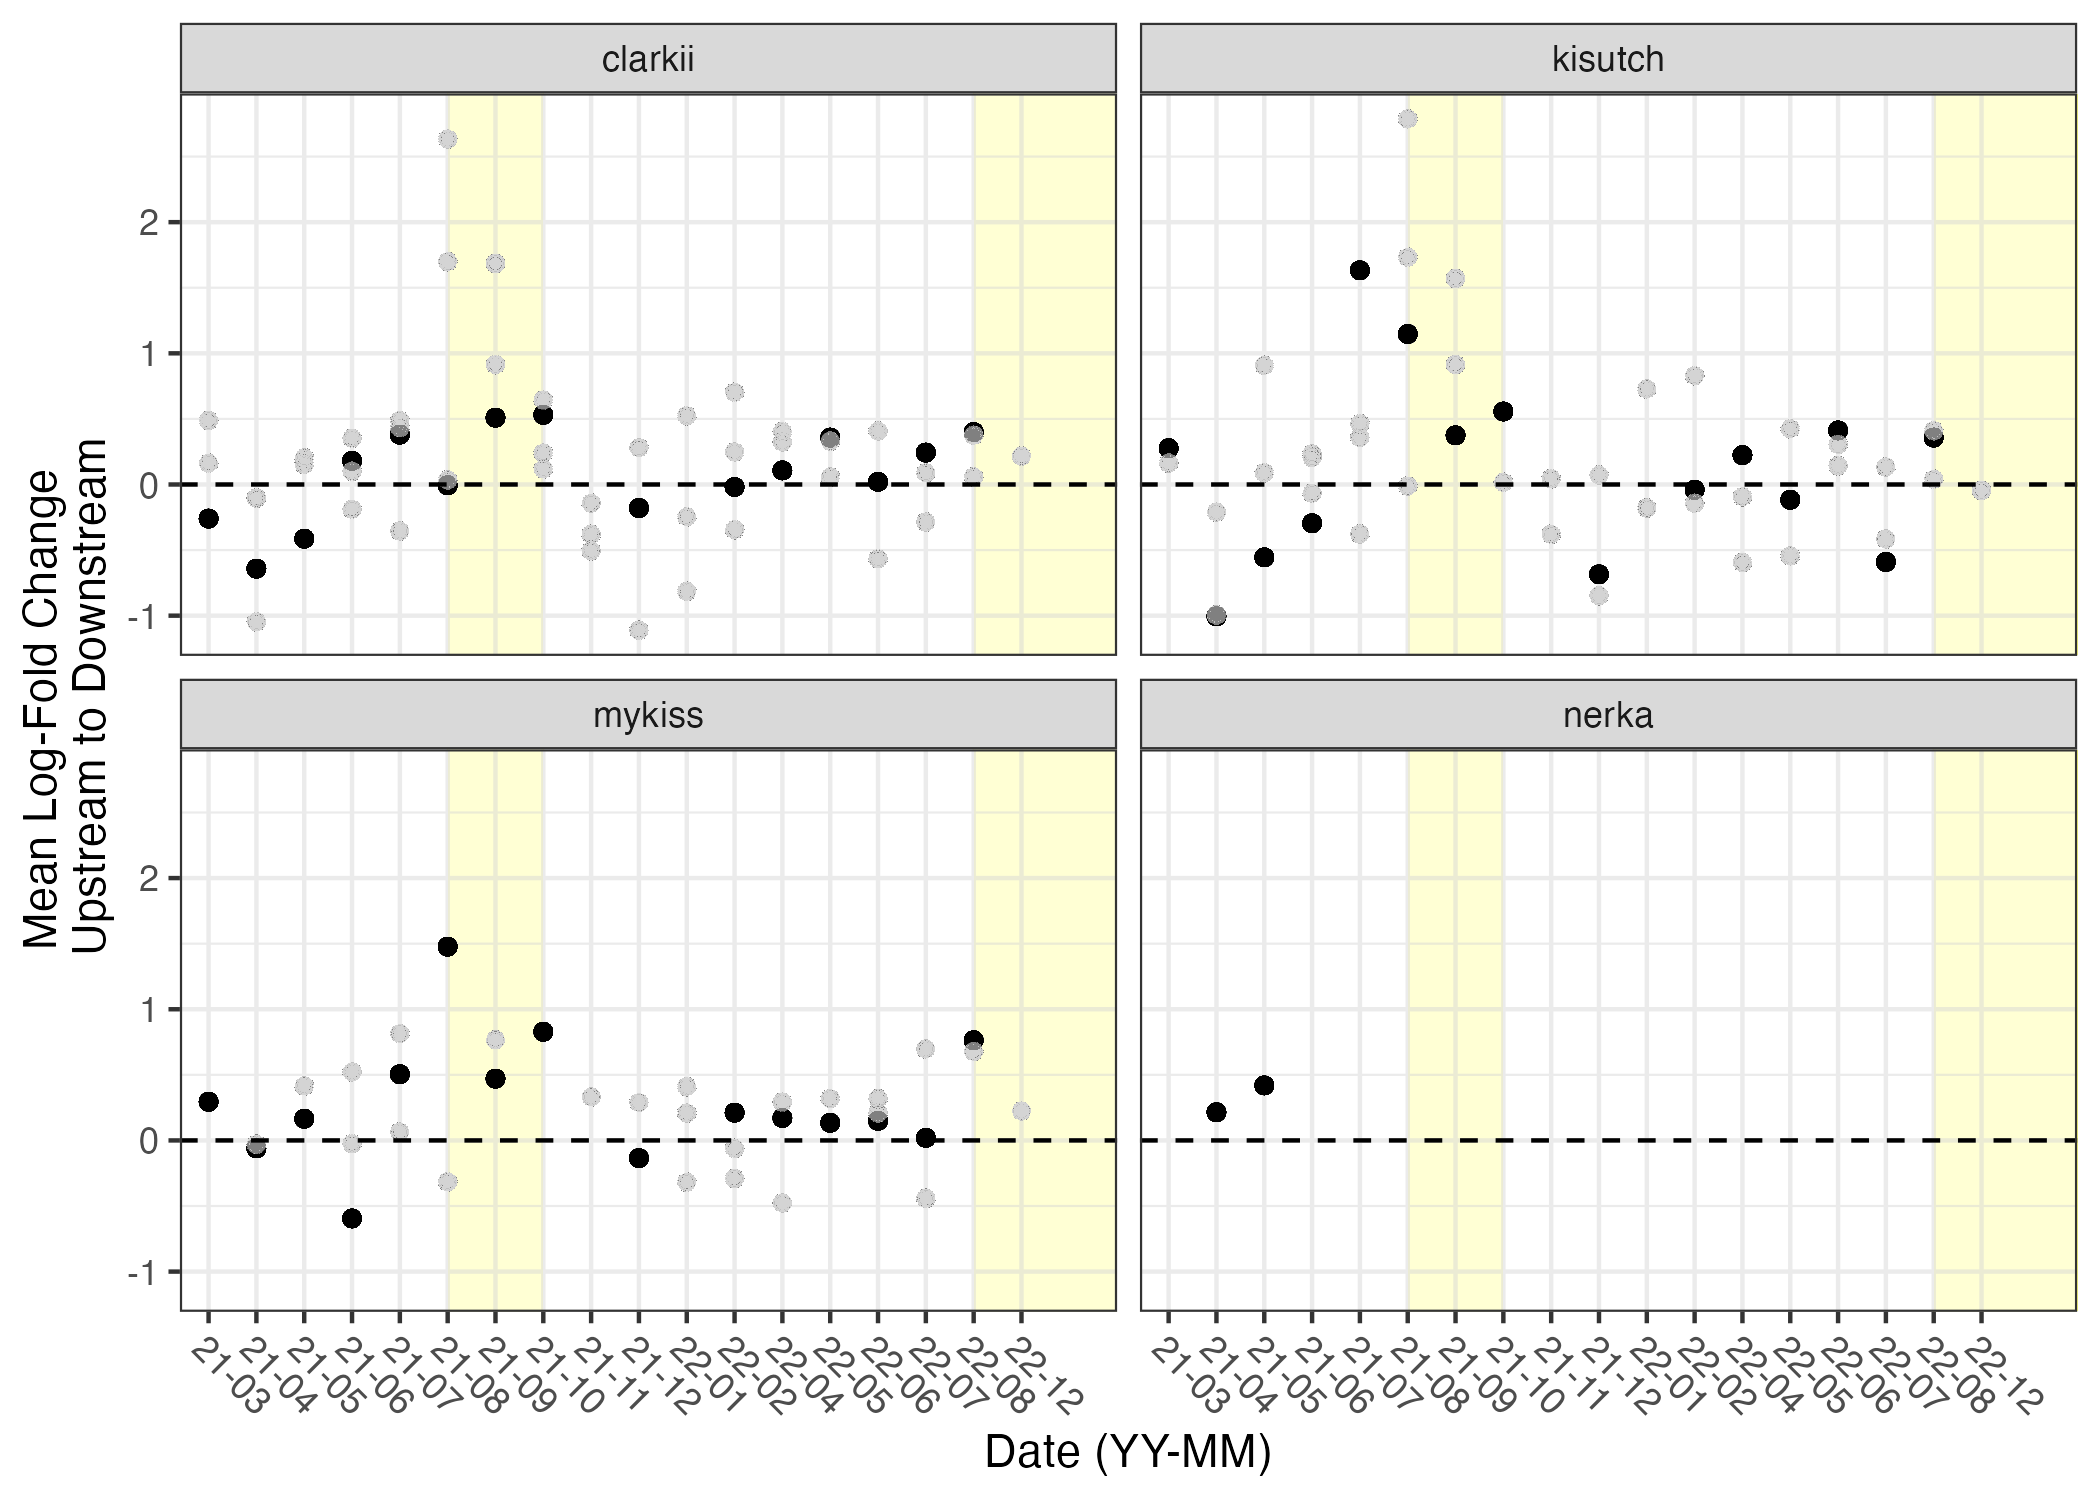
\includegraphics{../Output/Figures/culvert_padden_controls.png}
\DIFaddendFL \caption{Effect of Construction on \DIFdelbeginFL \DIFdelFL{Salmonid DNA Concentrations }\DIFdelendFL \DIFaddbeginFL \DIFaddFL{Log-Fold Change }\DIFaddendFL in \DIFaddbeginFL \DIFaddFL{eDNA Flow Rate
Upstream to Downstream in }\DIFaddendFL Padden Creek. \DIFdelbeginFL \DIFdelFL{Error bars show 95\% confidence intervals of the normalized
difference between upstream and downstream DNA concentrations. Grey
}\DIFdelendFL \DIFaddbeginFL \DIFaddFL{Yellow }\DIFaddendFL shading shows when
construction started \DIFdelbeginFL \DIFdelFL{through the end }\DIFdelendFL \DIFaddbeginFL \DIFaddFL{for each }\DIFaddendFL of \DIFdelbeginFL \DIFdelFL{sampling}\DIFdelendFL \DIFaddbeginFL \DIFaddFL{the two culverts}\DIFaddendFL . \DIFdelbeginFL \DIFdelFL{Construction ended }\DIFdelendFL \DIFaddbeginFL \DIFaddFL{Grey points show the
corresponding log-fold changes }\DIFaddendFL in \DIFdelbeginFL \DIFdelFL{early October 2022. }\DIFdelendFL \DIFaddbeginFL \DIFaddFL{control creeks and black points show
Padden Creek. Sockeye/kokanee salmon (}\DIFaddendFL \emph{O. nerka}\DIFaddbeginFL \DIFaddFL{) }\DIFaddendFL was only found in
Padden Creek so other creeks are not shown. \DIFaddbeginFL \DIFaddFL{Samples with very low eDNA
mass flow rates (\textless{} 150 copies/s) were removed before plotting
to remove extreme proportional values due to large
denomenators.}\DIFaddendFL \label{fig:construction}}

\end{figure}

\hypertarget{discussion}{%
\subsection{Discussion}\label{discussion}}

\hypertarget{environmental-dna-can-provide-quantitative-measurements-of-environmental-impacts}{%
\subsubsection{Environmental DNA can provide quantitative measurements
of environmental
impacts}\label{environmental-dna-can-provide-quantitative-measurements-of-environmental-impacts}}

Here, we used both eDNA metabarcoding and a single species-specific qPCR
assay to rigorously quantify both the effect of culverts and the impact
of \DIFdelbegin \DIFdel{a culvert replacement on salmonids }\DIFdelend \DIFaddbegin \DIFadd{two culvert replacements on salmonids in the same creek}\DIFaddend . We observed
a clear seasonal pattern in the DNA concentrations of four salmonid
species detected in the study. The \DIFdelbegin \DIFdel{BACI }\DIFdelend sampling design and the \DIFdelbegin \DIFdel{time series model leveraged shared information across }\DIFdelend \DIFaddbegin \DIFadd{linear mixed
effects model leveraged information across treatment and control }\DIFaddend creeks
to integrate the change in eDNA concentrations due to time, whether a
sample was collected below or above a barrier (i.e., culvert), and
whether or not there was construction occurring. Thus, we could isolate
the changes in eDNA concentrations as a result of the intervention
(i.e., construction) while accounting for the variance due to time and
station (i.e., season and culvert).

A few other studies have used eDNA to measure environmental impacts in
rivers and streams. Duda et al. (2021) used 11 species-specific qPCR
assays to document the distribution of resident and migratory fish after
a large dam removal \DIFdelbegin \DIFdel{(Elwah Dam in }\DIFdelend \DIFaddbegin \DIFadd{project (Elwha River near }\DIFaddend Port Angeles, Washington).
No eDNA sampling was conducted before the dam removal, but the study
provided a wealth of information about species returning after the dam
removal, providing a very important dataset to use eDNA to monitor
ecological changes due to human intervention. Similarly, Muha et al.
(2017) sampled three locations upstream and three locations downstream
before and after the removal of a weir that was thought to be a barrier
to salmonid migrations. The authors only sampled once before and twice
after the removal, spanning about a year, and used eDNA metabarcoding to
look at the presence/absence of species detected. They found that in
fact the before sample demonstrated that the weir was not preventing
fish passage (similar to the results found in this study) and
furthermore documented a slight increase in alpha diversity in the first
time point after the barrier removal and then a return to a similar
alpha diversity in the second time point after the removal (similar
results found in this study using eDNA concentrations rather than
diversity). \DIFaddbegin \DIFadd{Finally Yamanaka and Minamoto (2016) sampled along a river
with three barriers, finding some fish able to cross barriers and some
not, suggesting that the eDNA can indicated habitat connectivity for
fishes across barriers.
}\DIFaddend 

Importantly, our study demonstrates the value of combining a single qPCR
assay with metabarcoding data to generate quantitative estimates of eDNA
concentrations of many species without requiring \DIFdelbegin \DIFdel{n }\DIFdelend \DIFaddbegin \emph{\DIFadd{n}} \DIFaddend qPCR assays
for \DIFdelbegin \DIFdel{n
}\DIFdelend \DIFaddbegin \emph{\DIFadd{n}} \DIFaddend species of interest. Here, we ultimately only quantified
the impacts of four species, but importantly, we did not know \emph{a
priori} how many species of interest there might be and we reduced our
efforts two fold by only conducting two assays (one species-specific
qPCR and one metabarcoding assay) as opposed to four assays (four
species-specific qPCR assays). This can also be particularly helpful for
taxa that don't have a previously published qPCR assay, but are detected
using universal metabarcoding assays. Metabarcoding data alone only
gives compositional data, which cannot be used in a time series to
quantify environmental impacts because there is no information about
absolute eDNA concentrations. However, by anchoring or grounding
proportions using a single qPCR assay, the proportional data can be
turned into quantitative data. The species for which to run the qPCR
assay can be determined after the metabarcoding is completed; the most
commonly found species with a robust qPCR assay should be used to glean
the most information.

\hypertarget{fish-life-histories-and-expected-patterns}{%
\subsubsection{Fish life histories and expected
patterns}\label{fish-life-histories-and-expected-patterns}}

\DIFaddbegin \DIFadd{The four salmonid species in this study have different life histories
and behaviors that would impact when fish (and therefore eDNA
concentrations) occur in the creeks. Three of the four species in this
study have both freshwater and anadromous populations. Cutthroat trout
(}\emph{\DIFadd{O. clarkii}}\DIFadd{) encompasses both non-migrating, resident trout in
the creeks and coastal run cutthroat that migrate into Padden Creek from
saltwater (Bellingham Bay). Similarly, }\emph{\DIFadd{O. nerka}} \DIFadd{includes both
anadromous sockeye salmon and freshwater resident kokanee salmon and
}\emph{\DIFadd{O. mykiss}} \DIFadd{includes both anadromous steelhead trout and
non-migrating rainbow trout. Using eDNA, we cannot distinguish between
the migrating and non-migrating subspecies of }\emph{\DIFadd{O. clarkii}}\DIFadd{,
}\emph{\DIFadd{O. nerka}}\DIFadd{, and }\emph{\DIFadd{O. mykiss}}\DIFadd{. Therefore, our eDNA
concentrations might reflect contributions from both migrating and
non-migrating individuals at any given time point in the dataset.
}

\DIFadd{For these four anadromous salmonids, the run timings for the migrating
populations vary for each species in the study area (Bellingham, WA).
Adult coastal cutthroat (}\emph{\DIFadd{O. clarkii}}\DIFadd{) are documented to run
throughout the entire year, whereas coho salmon (}\emph{\DIFadd{O. kisutch}}\DIFadd{) run
from September to December, sockeye salmon (}\emph{\DIFadd{O. nerka}}\DIFadd{) run from
October to December, and steelhead trout (}\emph{\DIFadd{O. mykiss}}\DIFadd{) run from
November to June. For migrating coho (}\emph{\DIFadd{O. kisutch}}\DIFadd{) and steelhead
trout (}\emph{\DIFadd{O. mykiss}}\DIFadd{), juveniles may be present in the creeks
year-round (Figure S1.4). eDNA methods at present cannot distinguish
adults versus juveniles from DNA found in a water sample.
}

\DIFaddend Despite the mix of migrating and non-migrating populations and various
run timings, our metabarcoding data demonstrate that in Padden Creek,
there was a clear signal of \DIFaddbegin \DIFadd{sockeye/kokanee salmon (}\DIFaddend \emph{O. nerka}\DIFaddbegin \DIFadd{)
}\DIFaddend both upstream and downstream only in November 2021 - February 2022 \DIFdelbegin \DIFdel{(and
only upstream in March 2021).
}\DIFdelend \DIFaddbegin \DIFadd{and
again in December 2022. }\DIFaddend This signal corresponds well with the documented
run timing of October to December \DIFaddbegin \DIFadd{and the presence of out-migrating
juveniles in early spring}\DIFaddend . In contrast, \DIFaddbegin \DIFadd{cutthroat trout (}\DIFaddend \emph{O.
clarkii}\DIFdelbegin \DIFdel{and }\DIFdelend \DIFaddbegin \DIFadd{) and coho salmon (}\DIFaddend \emph{O. kisutch}\DIFaddbegin \DIFadd{) }\DIFaddend were found nearly
year-round in Padden Creek. The persistent signal from \emph{O. clarkii}
could be explained by resident cutthroat trout. However, \emph{O.
kisutch} does not have a resident subspecies and the run timing is only
documented from September to December. This could potentially be due to
juveniles maturing and residing in the creeks for 1-2 years after
hatching while adults migrate into the creeks only during the run time
to spawn. Visual surveys \DIFdelbegin \DIFdel{are conducted rarely and
even if they were conducted, it might be difficult to identify juveniles
to species level}\DIFdelend \DIFaddbegin \DIFadd{(e.g., snorkel surveys, electrofishing, smolt
traps) are conducted infrequently to determine adult and juvenile
salmonid abundances}\DIFaddend . Though \emph{O. kisutch} eDNA was found year round,
the highest concentrations were found near the expected run timing \DIFdelbegin \DIFdel{as
expected }\DIFdelend and
the life history of \emph{O. kisutch} includes rearing year-round in
freshwater. Finally, though the lowest concentrations on average,
\DIFaddbegin \DIFadd{rainbow/steelhead trout (}\DIFaddend \emph{O. mykiss}\DIFaddbegin \DIFadd{) }\DIFaddend was also found nearly
year-round in Padden Creek, which could be contributions from migrating
steelhead (November to June), juveniles maturing and migrating, or from
resident rainbow trout. Though the \emph{O. mykiss} signal is found
year-round, the highest concentrations do seem to correspond with the
steelhead run timing.

\DIFdelbegin %DIFDELCMD < \hypertarget{decoupling-of-edna-from-fish-abundance}{%
%DIFDELCMD < \subsubsection{Decoupling of eDNA from fish
%DIFDELCMD < abundance}\label{decoupling-of-edna-from-fish-abundance}}
%DIFDELCMD < %%%
\DIFdelend \DIFaddbegin \hypertarget{interpreting-edna-with-respect-to-fish-abundance-and-flow}{%
\subsubsection{Interpreting eDNA with respect to fish abundance and
flow}\label{interpreting-edna-with-respect-to-fish-abundance-and-flow}}
\DIFaddend 

By capturing residual eDNA from water samples, we are measuring a
different signal than counting how many fish are in the creek at each
time of sampling. We should not expect the eDNA concentration \DIFdelbegin \DIFdel{for each
salmonid }\DIFdelend to
directly correlate to the number of fish in the creek at the time of
sampling\DIFdelbegin \DIFdel{, especially as we often did not visually see any fish
when we took water samples}\DIFdelend . Shelton et al. (2019) \DIFdelbegin \DIFdel{provides }\DIFdelend \DIFaddbegin \DIFadd{used }\DIFaddend a paired eDNA sampling and seine
netting analysis \DIFdelbegin \DIFdel{demonstrating }\DIFdelend \DIFaddbegin \DIFadd{to demonstrate }\DIFaddend that eDNA concentrations provide a
smoothed biological signal over space and time. We acknowledge this
smoothing effect and emphasize that in the context of using eDNA for
environmental impact assessments, it is preferable to use a survey
technique such as eDNA that integrates signal across a larger spatial
and temporal scale.

Many previous papers have commented on the ``ecology'' of eDNA and the
various processes that contribute to eDNA concentrations in
environmental samples (e.g., shedding rates, decay rates, transport)
(Barnes and Turner 2015). For example, higher concentrations of eDNA
could be the result of a greater number (or biomass) of fish present, or
increased shedding rates, or decreased decay. Many review papers
document the nuances of interpreting eDNA data and we recommend
reviewing them for a deeper understanding (see Andruszkiewicz Allan et
al. (2020) for a review on shedding and decay rates and Harrison et al.
(2019) for a review on transport). \DIFaddbegin \DIFadd{Other studies have also documented
the relative importance of eDNA transport in streams. Most notably,
Tillotson et al. (2018) measured eDNA at four sites with similar
discharge rates to the creeks in this study and specifically addressed
spatial and temporal resolutions, finding that eDNA concentrations
reflect short time- (and therefore length-) scales by comparing peaks in
eDNA concentrations to counts of salmon and accumulation by measuring
both upstream and downstream sites. The authors found that the sampling
site furthest downstream did not accumulate eDNA and that two
tributaries feeding into a main channel were additive (Tillotson et al.
2018). For more general models and empirical data documenting transport
distances in streams, see Wilcox et al. (2016), Jane et al. (2014),
Jerde et al. (2016), Shogren et al. (2016), and Civade et al. (2016).
}\DIFaddend Certainly eDNA concentrations can arise from different scenarios and
future work should continue to investigate how to tease apart the
nuances of relating eDNA concentrations to fish abundance.

In this study, to assess the impact of a culvert on fish passage, we
compare eDNA concentrations upstream and downstream at the same time
point in a given creek. The distance between the upstream and downstream
sampling was minimal (\textasciitilde60-300 m, average distance of
\textasciitilde150 m). Therefore, we assume that the small differences
in spatial and temporal scale between sampling locations is minimal such
that the impacts of these various processes will affect the downstream
and upstream concentrations equally. \DIFdelbegin %DIFDELCMD < 

%DIFDELCMD < %%%
\DIFdel{For assessing the impact of construction, we needed to account for
differences within the same creek over time (i.e., before and after
construction). Because the sampling occurred over a whole year,
transport and persistence times may have varied. However, the time
series model uses information from the control creeks to understand
seasonal trends in eDNA concentrations without needing to link eDNA
concentrations to fish abundance. The impact of construction in Padden
Creek can be understood by comparing the measured eDNA concentration
during the time of construction to the expected eDNA concentration in
the absence of construction by using information shared from the four
other creeks that are not undergoing construction. However, we did
correct eDNA concentrations }%DIFDELCMD < {[}%%%
\DIFdel{mass/volume}%DIFDELCMD < {]} %%%
\DIFdel{by discharge
}%DIFDELCMD < {[}%%%
\DIFdel{volume/time}%DIFDELCMD < {]} %%%
\DIFdel{and use a mass flow rate }%DIFDELCMD < {[}%%%
\DIFdel{mass/time}%DIFDELCMD < {]} %%%
\DIFdel{for the time
series model (see below) given the wide range of discharge over the
course of the year.
}%DIFDELCMD < 

%DIFDELCMD < \hypertarget{accounting-for-flow-with-edna-concentrations}{%
%DIFDELCMD < \subsubsection{Accounting for flow with eDNA
%DIFDELCMD < concentrations}\label{accounting-for-flow-with-edna-concentrations}}
%DIFDELCMD < 

%DIFDELCMD < %%%
\DIFdel{Though eDNA can move downstream with water flow, here, we were measuring
if culverts were barriers to fish moving upstream, as we were focused on
the impact of culverts on migratory salmon. In our case, we were
comparing if downstream stations had higher DNA concentrations than
upstream stations as a result of fish being unable to get upstream. This
is of course complicated as a result of non-migratory fish, which may be
up or downstream and not attempting to pass through the culverts.
However, the limited spatial scale between upstream and downstream is
such that we can assume the transport would affect upstream and
downstream locations in the same way. }\DIFdelend That is, in the upstream station,
some amount of eDNA is coming from upstream of that location into the
sampling station and leaving at the same time \DIFdelbegin \DIFdel{--- }\DIFdelend \DIFaddbegin \DIFadd{-- }\DIFaddend in the same way that
eDNA would be both entering and exiting the downstream station.
\DIFdelbegin \DIFdel{Therefore, the relative change between upstream and downstream stations
should be the same in terms of eDNA transport. }\DIFdelend Additionally, at almost every single time point for all creeks and
species, the upstream DNA concentration is higher than the downstream
DNA concentration. Based on that alone, we do not expect that downstream
accumulation of salmonid DNA is occurring to bias our results of whether
fish can pass through these culverts.

\DIFdelbegin \DIFdel{Other studies have documented the relative importance of eDNA transport
in streams. Most notably, Tillotson et al. (2018) measured eDNA at four
sites with similar discharge rates to the creeks in this study and
specifically addressed spatial and temporal resolutions, finding that
eDNA concentrations reflect short time- (and therefore length-) scales
by comparing peaks in eDNA concentrations to counts of salmon and
accumulation by measuring both upstream and downstream sites. The
authors found that the sampling site furthest downstream did not
accumulate eDNA and that two tributaries feeding into a main channel
were additive (Tillotson et al. 2018). For more general models and
empirical data documenting transport distances in streams, see Wilcox et
al. (2016), Jane et al. (2014), Jerde et al. (2016), Shogren et al.
(2016), and Civade et al. (2016).
}%DIFDELCMD < 

%DIFDELCMD < %%%
\DIFdel{Finally, it should be noted that Lake Padden, about 1.5 km upstream from
the sampling sites, was stocked with cutthroat trout in January 2021,
rainbow trout in April and May 2021, and kokanee salmon in May 2021.
Given that no sequencing reads in the metabarcoding data are found for
}\emph{\DIFdel{O. nerka}} %DIFAUXCMD
\DIFdel{in May or June after stocking in May, the potential
transport of eDNA downstream from Lake Padden to the location of eDNA
sampling is expected to be negligible. Given the transport distances
documented in the literature and flow rates in Lake Padden, we do not
expect the stocking in Lake Padden to affect eDNA concentrations at the
sampling locations.
}%DIFDELCMD < 

%DIFDELCMD < %%%
\DIFdelend \hypertarget{not-all-culverts-are-barriers-to-salmonids}{%
\subsubsection{Not all culverts are barriers to
salmonids}\label{not-all-culverts-are-barriers-to-salmonids}}

By measuring DNA concentrations of salmonid species above and below
culverts on a small spatial scale, we were able to determine how much of
a barrier each culvert was \DIFdelbegin \DIFdel{(or was not) }\DIFdelend to fish passage. \DIFdelbegin \DIFdel{We found by
measuring eDNA concentrations that four of the five creeks sampled did
not seem to be major barriers to fish passage. The only creek that was determined to be a
}\DIFdelend \DIFaddbegin \DIFadd{Barnes Creek was clearly a
very large }\DIFaddend barrier to fish passage \DIFdelbegin \DIFdel{was Barnes Creek, }\DIFdelend as we only found salmonid DNA in
three months of the twelve months of sampling, and those three months
had very low concentration of salmonid DNA relative to the other creeks.
\DIFdelbegin \DIFdel{We note that our sampling occurred only over a
single year and future work should monitor culverts for longer time
periods, different species, and different environmental conditions.
}%DIFDELCMD < 

%DIFDELCMD < %%%
\DIFdel{Of the four creeks where salmonid DNA was consistently found, Chuckanut
Creekhad the largest discrepancies between DNA concentrations found
below and above the barrier at each time point. The culvert in Chuckanut
Creek is suspected }\DIFdelend \DIFaddbegin \DIFadd{Within the treatment creek (Padden Creek), the SR-11 culvert did not
seem }\DIFaddend to be a \DIFdelbegin \DIFdel{barrier to fish passage and the State of
Washington's Department of Transportation is planning to replace it in
the near future. The bridge at Portage Creek and the culvert at
Squalicum Creek were more recently installed as compared to Padden,
Chuckanut, and Barnes Creeks. They also were designated as only
partially blocking fish passage, and here we find eDNA results suggest
that they were in fact not major barriers to fish passage. Squalicum
Creek had the lowest difference between upstream and downstream
concentrations across all the surveyed creeks, which corresponds well
with the classification that the culvert does not block fish passage.
Also, Squalicum Creek is the only creek sampled that has baffles inside
the culvert, which should help fish passage.
}\DIFdelend \DIFaddbegin \DIFadd{large barrier, while the I-5 culvert clearly was a barrier,
demonstrated by the difference in salmonid composition and eDNA mass
flow rates over the course of sampling.
}\DIFaddend 

Here, we find \DIFdelbegin \DIFdel{that }\DIFdelend \DIFaddbegin \DIFadd{instances where }\DIFaddend culverts designated as barriers were
likely not blocking fish passage\DIFaddbegin \DIFadd{, while others (Padden I-5 and Barnes
Creek) were barriers to fish passage}\DIFaddend . Importantly, this demonstrates
that collecting water samples for eDNA analysis might help to prioritize
restoration of culverts suspected to be barriers to salmonids and
provide a new method for post-restoration monitoring to confirm that the
barrier has been corrected and allows for fish passage. Given the large
amount of spending and effort required to replace culverts, this finding
is important and emphasizes the potential for new tools for
environmental impact assessments. \DIFaddbegin \DIFadd{We note that our sampling occurred
only over a short temporal scale and future work could monitor culverts
for longer time periods, different species, and different environmental
conditions.
}\DIFaddend 

\hypertarget{salmonids-can-quickly-recover-from-a-short-term-intervention-in-a-creek}{%
\subsubsection{Salmonids can quickly recover from a short-term
intervention in a
creek}\label{salmonids-can-quickly-recover-from-a-short-term-intervention-in-a-creek}}

The \DIFdelbegin \DIFdel{impact of the construction itself on salmonid species demonstrated
}\DIFdelend \DIFaddbegin \DIFadd{construction had }\DIFaddend remarkably minimal effects on salmonid DNA
concentrations. The disruption of disconnecting \DIFdelbegin \DIFdel{Padden Creek in late August}\DIFdelend \DIFaddbegin \DIFadd{the creek}\DIFaddend , demolition of
the old culvert, installation of the new culvert, and the reconnecting
of the creek \DIFdelbegin \DIFdel{in early October 2021 }\DIFdelend \DIFaddbegin \DIFadd{during both culvert replacement events }\DIFaddend showed almost no
change in the difference in eDNA concentrations between downstream and
upstream sampling sites. The differences in the control creeks between
upstream and downstream were often higher than the treatment creek. \DIFdelbegin %DIFDELCMD < 

%DIFDELCMD < %%%
\DIFdel{The
construction timing did coincide with natural life history cycles
for the salmon species. In the fall an influx of DNA would be expected
not only from adults returning to spawn as they move through the system, but also from the presence of spawning material in the creek and
decaying adults that die post reproduction. This may explain a portion
of the changes in DNA concentrations found here as the construction
timing coincided with run timings of the salmonids, however our time
series model accounts for changes in season in attempt to isolate the effects of the culvert and construction. Regardless, the changes between
upstream and downstream concentrations were very minor across time
points and before and after construction }\DIFdelend \DIFaddbegin \DIFadd{The
post-construction sampling point of the I-5 culvert replacement (only
one time point), does show that the composition of salmonid DNA after
replacement is now very similar to the two downstream stations, whereas
before construction compositions were very different (because the
culvert was a barrier)}\DIFaddend . \DIFdelbegin %DIFDELCMD < 

%DIFDELCMD < %%%
\DIFdel{This pattern of minimal disruption and quick recovery was consistent for
all four species of salmonids, but the
more abundant species seemed to
have a dampened effect (i.e., less overall change)compared to the rarer
species (i. e., }\emph{\DIFdel{O. clarkii}} %DIFAUXCMD
\DIFdel{was the least impacted and }\emph{\DIFdel{O.
nerka}} %DIFAUXCMD
\DIFdel{was the most impacted). This also corresponds to species with
different life histories and behaviors, and it might be that our most
commonly and abundant species, }\emph{\DIFdel{O. clarkii}}%DIFAUXCMD
\DIFdel{, was more robust to the
intervention because it displays both freshwater resident and saltwater
migrating behaviors. }%DIFDELCMD < 

%DIFDELCMD < %%%
\DIFdel{Our findings here demonstrate that in addition to the value of using
eDNA to select culverts to prioritize for replacement, sampling during
and after construction can provide important information about the
impacts (or lack of impacts) on salmonids}\DIFdelend \DIFaddbegin \DIFadd{However, we lack the quantitative analysis as
the site upstream of SR-11 and downstream of I-5 had no quantifiable
cutthroat DNA. More time points would help demonstrate the effect of the
culvert replacement}\DIFaddend . Here we found \DIFdelbegin \DIFdel{very minimal
effects of both culverts in general and construction, but }\DIFdelend \DIFaddbegin \DIFadd{that one culvert had very minimal
effect on salmonid passage while the other culvert had a large effect on
salmonid passage. We note that }\DIFaddend these findings are likely not universal
and certainly projects need to monitor comprehensively and
quantitatively in order to assess the passability of culverts and
impacts of construction.

\hypertarget{conclusion}{%
\subsection{Conclusion}\label{conclusion}}

It is notoriously difficult to quantify the environmental impact of
discrete human impacts on ecosystems and species. Surveying species and
communities by eDNA provides an opportunity for monitoring before,
during, and after impacts in a scaleable and cost-effective way. Here,
we demonstrate that monthly eDNA sampling before, during, and after an
intervention alongside control sites \DIFdelbegin \DIFdel{for one year }\DIFdelend can quantify the environmental
impact of replacing a \DIFdelbegin \DIFdel{road }\DIFdelend culvert. We found that in our treatment creek and
control sites, four of the \DIFdelbegin \DIFdel{five }\DIFdelend \DIFaddbegin \DIFadd{six }\DIFaddend barriers did not prohibit salmonid
passage\DIFdelbegin \DIFdel{and that the culvert replacement }\DIFdelend \DIFaddbegin \DIFadd{. We found that of the two culvert replacements }\DIFaddend in the treatment
creek\DIFaddbegin \DIFadd{, one was a barrier and one was not, but both }\DIFaddend had minimal impacts
on the four salmonid species monitored \DIFaddbegin \DIFadd{over the course of construction}\DIFaddend .
We also provide a framework in which compositional metabarcoding data
can be linked with qPCR data to obtain quantitative estimates of eDNA
concentrations of many species. This provides a practical way to utilize
the large amount of information from metabarcoding data without needing
a unique qPCR assay for every species of interest. Environmental DNA is
moving into practice and this study demonstrates how eDNA can be broadly
used for environmental impact assessments for a wide range of species
and environments.

\hypertarget{conflict-of-interest-statement}{%
\subsection{Conflict of Interest
Statement}\label{conflict-of-interest-statement}}

The authors declare there are no conflicts of interest.

\hypertarget{acknowledgements}{%
\subsection{Acknowledgements}\label{acknowledgements}}

This work was made possible by a grant from \DIFdelbegin \DIFdel{the National Philanthropic
Trust }\DIFdelend \DIFaddbegin \DIFadd{OceanKind }\DIFaddend to Ryan Kelly. The
funders had no role in study design, data collection and analysis,
decision to publish, or preparation of the manuscript. \DIFaddbegin \DIFadd{Figure 3 was
created with BioRender.com. }\DIFaddend We thank Tammy Schmidt and Susan Kanzler
from Washington Department of Transportation for facilitating access to
field sites and providing helpful feedback throughout the project. We
also thank \DIFdelbegin \DIFdel{Dr.~}\DIFdelend Jenna McLaughlin, Joe Duprey and Ally Im for help field
sampling and Dr.~Ramon Gallego, Dr.~Kim Parsons, and the University of
Washington's Northwest Genomics Center for sequencing support.
Dr.~Braeden Van Deynze, Dr.~Sunny Jardine, and Dr.~Julian Olden provided
helpful insight into culverts and salmonid life histories. \DIFaddbegin \DIFadd{We thank
Katherine Pearson Maslenikov at the Burke Museum of Natural History and
Culture for providing voucher specimens for Sanger sequencing. }\DIFaddend Thanks to
Dr.~Jameal Samhouri \DIFdelbegin \DIFdel{for reviewing the manuscript. A special thank you to }\DIFdelend \DIFaddbegin \DIFadd{and }\DIFaddend Dr.~Chris Sergeant for \DIFdelbegin \DIFdel{providing feedback throughout the project and improving the
}\DIFdelend \DIFaddbegin \DIFadd{reviewing the }\DIFaddend manuscript.

\hypertarget{references}{%
\subsection*{References}\label{references}}
\addcontentsline{toc}{subsection}{References}

\hypertarget{refs}{}
\begin{CSLReferences}{1}{0}
\leavevmode\vadjust pre{\hypertarget{ref-andruszkiewiczallan2020}{}}%
Andruszkiewicz Allan, E., W. G. Zhang, A. Lavery, and A. Govindarajan.
2020. \href{https://doi.org/10.1002/edn3.141}{Environmental DNA shedding
and decay rates from diverse animal forms and thermal regimes}.
Environmental DNA:edn3.141.

\leavevmode\vadjust pre{\hypertarget{ref-barnes2015}{}}%
Barnes, M. A., and C. R. Turner. 2015. The ecology of environmental DNA
and implications for conservation genetics. Conservation Genetics
17:117.

\leavevmode\vadjust pre{\hypertarget{ref-benedetti-cecchi2001}{}}%
Benedetti-Cecchi, L. 2001.
\href{https://doi.org/10.1890/1051-0761(2001)011\%5B0783:BBOOES\%5D2.0.CO;2}{Beyond
Baci: Optimization of Environmental Sampling Designs Through Monitoring
and Simulation}. Ecological Applications 11:783--799.

\leavevmode\vadjust pre{\hypertarget{ref-buxton2021}{}}%
Buxton, A., E. Matechou, J. Griffin, A. Diana, and R. A. Griffiths.
2021. \href{https://doi.org/10.1038/s41598-021-91166-7}{Optimising
sampling and analysis protocols in environmental DNA studies}.
Scientific Reports 11:11637.

\leavevmode\vadjust pre{\hypertarget{ref-callahan2016}{}}%
Callahan, B. J., P. J. McMurdie, M. J. Rosen, A. W. Han, A. J. A.
Johnson, and S. P. Holmes. 2016.
\href{https://doi.org/10.1038/nmeth.3869}{DADA2: High resolution sample
inference from illumina amplicon data}. Nature methods 13:581--583.

\leavevmode\vadjust pre{\hypertarget{ref-camacho2009}{}}%
Camacho, C., G. Coulouris, V. Avagyan, N. Ma, J. Papadopoulos, K.
Bealer, and T. L. Madden. 2009. BLAST+: Architecture and applications.
BMC Bioinformatics 10:4219.

\leavevmode\vadjust pre{\hypertarget{ref-cityofbellingham2015}{}}%
City of Bellingham. 2015. Urban spawner surveys.

\leavevmode\vadjust pre{\hypertarget{ref-civade2016}{}}%
Civade, R. l., T. Dejean, A. Valentini, N. Roset, J.-C. Raymond, A.
Bonin, P. Taberlet, and D. Pont. 2016. Spatial representativeness of
environmental DNA metabarcoding signal for fish biodiversity assessment
in a natural freshwater system. PLOS ONE 11:e015736619.

\leavevmode\vadjust pre{\hypertarget{ref-devargas2015}{}}%
De Vargas, C., S. Audie, N. Henry, J. Decelle, F. Mahe, R. Logares, E.
Lara, C. Berney, N. Le Bescot, I. Probert, M. Carmichael, J. Poulain, S.
Romac, S. Colin, J.-M. Aury, L. Bittner, S. Chaffron, M. Dunthorn, S.
Engelen, O. Flegontova, L. Guidi, A. Horak, O. Jaillon, G. Lima-Mendez,
J. Lukes, S. Malviya, R. Morard, M. Mulot, E. Scalco, R. Siano, F.
Vincent, A. Zingone, C. Dimier, M. Picheral, S. Searson, S.
Kandels-Lewis, T. O. coordinators, S. G. Acinas, P. Bork, C. Bowler, G.
Gorsky, N. Grimsley, P. Hingamp, D. Iudicone, F. Not, H. Ogata, S.
Pesant, J. Raes, M. E. Sieracki, S. Speich, L. Stemmann, S. Sunagawa, J.
Weissenbach, P. Wincker, and E. Karsenti. 2015. Eukaryotic plankton
diversity in the sunlit ocean. Science 348:112.

\leavevmode\vadjust pre{\hypertarget{ref-duda2021}{}}%
Duda, J. J., M. S. Hoy, D. M. Chase, G. R. Pess, S. J. Brenkman, M. M.
McHenry, and C. O. Ostberg. 2021.
\href{https://doi.org/10.1002/edn3.134}{Environmental DNA is an
effective tool to track recolonizing migratory fish following
large-scale dam removal}. Environmental DNA 3:121--141.

\leavevmode\vadjust pre{\DIFdelbegin %DIFDELCMD < \hypertarget{ref-washingtondepartmentoffishandwildlife2019}{}}%%%
%DIF < 
\DIFdel{Fish, W. D. of, and Wildlife. 2019a. Fish passage inventory, assessment,
and prioritization manual.
}%DIFDELCMD < 

%DIFDELCMD < \leavevmode\vadjust %%%
\DIFdel{pre}%DIFDELCMD < {\hypertarget{ref-washingtondepartmentoffishandwildlife2019a}{}}%%%
%DIF < 
\DIFdel{Fish, W. D. of, and Wildlife. 2019b. Fish passage inventory, assessment,
and prioritization manual.
}%DIFDELCMD < 

%DIFDELCMD < \leavevmode\vadjust %%%
\DIFdel{pre}%DIFDELCMD < {%%%
\DIFdelend \hypertarget{ref-frankiewicz2021}{}}%
Frankiewicz, P., A. Radecki-Pawlik, A. Wałęga, M. Łapińska, and A.
Wojtal-Frankiewicz. 2021.
\href{https://doi.org/10.1139/er-2020-0126}{Small hydraulic structures,
big environmental problems: is it possible to mitigate the negative
impacts of culverts on stream biota?} Environmental Reviews 29:510--528.

\leavevmode\vadjust pre{\hypertarget{ref-gloor2016}{}}%
Gloor, G. B., J. M. Macklaim, M. Vu, and A. D. Fernandes. 2016.
\href{https://doi.org/10.17713/ajs.v45i4.122}{Compositional uncertainty
should not be ignored in high-throughput sequencing data analysis}.
Austrian Journal of Statistics 45:73--87.

\leavevmode\vadjust pre{\DIFaddbegin \hypertarget{ref-gold2023}{}}%DIF > 
\DIFadd{Gold, Z., A. O. Shelton, H. R. Casendino, J. Duprey, R. Gallego, A. V.
Cise, M. Fisher, A. J. Jensen, E. D'Agnese, E. A. Allan, A. Ramón-Laca,
M. Garber-Yonts, M. Labare, K. M. Parsons, and R. P. Kelly. 2023.
}\href{https://doi.org/10.1371/journal.pone.0285674}{\DIFadd{Signal and noise in
metabarcoding data}}\DIFadd{. PLOS ONE 18:e0285674.
}

\leavevmode\vadjust \DIFadd{pre}{\DIFaddend \hypertarget{ref-harrison2019}{}}%
Harrison, J. B., J. M. Sunday, and S. M. Rogers. 2019.
\href{https://doi.org/10.1098/rspb.2019.1409}{Predicting the fate of
eDNA in the environment and implications for studying biodiversity}.
Proceedings of the Royal Society B: Biological Sciences 286:20191409.

\leavevmode\vadjust pre{\DIFdelbegin %DIFDELCMD < \hypertarget{ref-hinz2022}{}%%%
\DIFdelend \DIFaddbegin \hypertarget{ref-hoshino2021}{}\DIFaddend }%
\DIFdelbegin \DIFdel{Hinz, S., J. Coston-Guarini, M. Marnane, and J. -M. Guarini. 2022.
}\href{https://doi.org/10.3390/jmse10030375}{\DIFdel{Evaluating eDNA for Use
within Marine Environmental Impact Assessments}}%DIFAUXCMD
\DIFdel{. Journal of Marine
Science and Engineering 10:375.
}\DIFdelend \DIFaddbegin \DIFadd{Hoshino, T., R. Nakao, H. Doi, and T. Minamoto. 2021.
}\href{https://doi.org/10.1038/s41598-021-83318-6}{\DIFadd{Simultaneous absolute
quantification and sequencing of fish environmental DNA in a mesocosm by
quantitative sequencing technique}}\DIFadd{. Scientific Reports 11:4372.
}\DIFaddend 

\leavevmode\vadjust pre{\hypertarget{ref-jane2014}{}}%
Jane, S. F., T. M. Wilcox, K. S. McKelvey, M. K. Young, M. K. Schwartz,
W. H. Lowe, B. H. Letcher, and A. R. Whiteley. 2014. Distance, flow and
PCR inhibition: eDNA dynamics in two headwater streams. Molecular
Ecology Resources 15:216227.

\leavevmode\vadjust pre{\hypertarget{ref-jerde2016}{}}%
Jerde, C. L., B. P. Olds, A. J. Shogren, E. A. Andruszkiewicz, A. R.
Mahon, D. Bolster, and J. L. Tank. 2016. Influence of stream bottom
substrate on retention and transport of vertebrate environmental DNA.
Environmental Science \& Technology 50:87708779.

\leavevmode\vadjust pre{\hypertarget{ref-kelly2017}{}}%
Kelly, R. P., C. J. Closek, J. L. O'Donnell, J. E. Kralj, A. O. Shelton,
and J. F. Samhouri. 2017. Genetic and manual survey methods yield
different and complementary views of an ecosystem. Frontiers in Marine
Science 3:73511.

\leavevmode\vadjust pre{\hypertarget{ref-kelly2014}{}}%
Kelly, R. P., J. A. Port, K. M. Yamahara, and L. B. Crowder. 2014. Using
environmental DNA to census marine fishes in a large mesocosm. PLOS ONE
9:e8617511.

\leavevmode\vadjust pre{\hypertarget{ref-kelly2019}{}}%
Kelly, R. P., A. O. Shelton, and R. Gallego. 2019.
\href{https://doi.org/10.1038/s41598-019-48546-x}{Understanding PCR
Processes to Draw Meaningful Conclusions from Environmental DNA
Studies}. Scientific Reports 9:12133.

\leavevmode\vadjust pre{\hypertarget{ref-klein2022}{}}%
Klein, S. G., N. R. Geraldi, A. Anton, S. Schmidt-Roach, M. Ziegler, M.
J. Cziesielski, C. Martin, N. Rädecker, T. L. Frölicher, P. J. Mumby, J.
M. Pandolfi, D. J. Suggett, C. R. Voolstra, M. Aranda, and Carlos. M.
Duarte. 2022. \href{https://doi.org/10.1111/gcb.15818}{Projecting coral
responses to intensifying marine heatwaves under ocean acidification}.
Global Change Biology 28:1753--1765.

\leavevmode\vadjust pre{\hypertarget{ref-lackey2003}{}}%
Lackey, R. 2003.
\href{https://doi.org/10.1080/16226510390856529}{Pacific Northwest
Salmon: Forecasting Their Status in 2100}. Reviews in Fisheries Science
11:35--88.

\leavevmode\vadjust pre{\hypertarget{ref-leray2013}{}}%
Leray, M., J. Y. Yang, C. P. Meyer, S. C. Mills, N. Agudelo, V. Ranwez,
J. T. Boehm, and R. J. Machida. 2013. A new versatile primer set
targeting a short fragment of the mitochondrial COI region for
metabarcoding metazoan diversity: Application for characterizing coral
reef fish gut contents. Frontiers in Zoology 10:114.

\leavevmode\vadjust pre{\hypertarget{ref-long2018}{}}%
Long, J. W., and F. K. Lake. 2018.
\href{https://www.jstor.org/stable/26799109}{Escaping social-ecological
traps through tribal stewardship on national forest lands in the pacific
northwest, united states of america}. Ecology and Society 23.

\leavevmode\vadjust pre{\hypertarget{ref-maasri2022}{}}%
Maasri, A., S. C. Jähnig, M. C. Adamescu, R. Adrian, C. Baigun, D. J.
Baird, A. Batista-Morales, N. Bonada, L. E. Brown, Q. Cai, J. V.
Campos-Silva, V. Clausnitzer, T. Contreras-MacBeath, S. J. Cooke, T.
Datry, G. Delacámara, L. De Meester, K.-D. B. Dijkstra, V. T. Do, S.
Domisch, D. Dudgeon, T. Erös, H. Freitag, J. Freyhof, J. Friedrich, M.
Friedrichs-Manthey, J. Geist, M. O. Gessner, P. Goethals, M. Gollock, C.
Gordon, H.-P. Grossart, G. Gulemvuga, P. E. Gutiérrez-Fonseca, P. Haase,
D. Hering, H. J. Hahn, C. P. Hawkins, F. He, J. Heino, V. Hermoso, Z.
Hogan, F. Hölker, J. M. Jeschke, M. Jiang, R. K. Johnson, G. Kalinkat,
B. K. Karimov, A. Kasangaki, I. A. Kimirei, B. Kohlmann, M. Kuemmerlen,
J. J. Kuiper, B. Kupilas, S. D. Langhans, R. Lansdown, F. Leese, F. S.
Magbanua, S. S. Matsuzaki, M. T. Monaghan, L. Mumladze, J. Muzon, P. A.
Mvogo Ndongo, J. C. Nejstgaard, O. Nikitina, C. Ochs, O. N. Odume, J. J.
Opperman, H. Patricio, S. U. Pauls, R. Raghavan, A. Ramírez, B. Rashni,
V. Ross-Gillespie, M. J. Samways, R. B. Schäfer, A. Schmidt-Kloiber, O.
Seehausen, D. N. Shah, S. Sharma, J. Soininen, N. Sommerwerk, J. D.
Stockwell, F. Suhling, R. D. Tachamo Shah, R. E. Tharme, J. H. Thorp, D.
Tickner, K. Tockner, J. D. Tonkin, M. Valle, J. Vitule, M. Volk, D.
Wang, C. Wolter, and S. Worischka. 2022.
\href{https://doi.org/10.1111/ele.13931}{A global agenda for advancing
freshwater biodiversity research}. Ecology Letters 25:255--263.

\leavevmode\vadjust pre{\hypertarget{ref-macpherson2012}{}}%
MacPherson, L. M., M. G. Sullivan, A. Lee Foote, and C. E. Stevens.
2012. \href{https://doi.org/10.1080/02755947.2012.686004}{Effects of
Culverts on Stream Fish Assemblages in the Alberta Foothills}. North
American Journal of Fisheries Management 32:480--490.

\leavevmode\vadjust pre{\hypertarget{ref-martin2012}{}}%
Martin, C. J. B., B. J. Allen, and C. G. Lowe. 2012.
\href{https://doi.org/10.3160/0038-3872-111.2.119}{Environmental impact
assessment: Detecting changes in fish community structure in response to
disturbance with an asymmetric multivariate BACI sampling design}.
Bulletin, Southern California Academy of Sciences 111:119--131.

\leavevmode\vadjust pre{\hypertarget{ref-martin2011}{}}%
Martin, M. 2011. \href{https://doi.org/10.14806/ej.17.1.200}{Cutadapt
removes adapter sequences from high-throughput sequencing reads}.
EMBnet.journal 17:10.

\leavevmode\vadjust pre{\hypertarget{ref-martinez2013}{}}%
Martinez, R. 2013. United states v. washington.

\leavevmode\vadjust pre{\hypertarget{ref-mccall2014}{}}%
McCall, M. N., H. R. McMurray, H. Land, and A. Almudevar. 2014.
\href{https://doi.org/10.1093/bioinformatics/btu239}{On non-detects in
qPCR data}. Bioinformatics 30:2310--2316.

\leavevmode\vadjust pre{\hypertarget{ref-mclaren2019}{}}%
McLaren, M. R., A. D. Willis, and B. J. Callahan. 2019.
\href{https://doi.org/10.7554/eLife.46923}{Consistent and correctable
bias in metagenomic sequencing experiments}. eLife 8:e46923.

\leavevmode\vadjust pre{\hypertarget{ref-morgan2012}{}}%
Morgan, R. K. 2012.
\href{https://doi.org/10.1080/14615517.2012.661557}{Environmental impact
assessment: The state of the art}. Impact Assessment and Project
Appraisal 30:5--14.

\leavevmode\vadjust pre{\hypertarget{ref-moss2022}{}}%
Moss, W. E., L. R. Harper, M. A. Davis, C. S. Goldberg, M. M. Smith, and
P. T. J. Johnson. 2022.
\href{https://doi.org/10.1002/ecs2.3941}{Navigating the trade-offs
between environmental DNA and conventional field surveys for improved
amphibian monitoring}. Ecosphere 13:e3941.

\leavevmode\vadjust pre{\hypertarget{ref-muha2017}{}}%
Muha, T. P., M. Rodríguez-Rey, M. Rolla, and E. Tricarico. 2017. Using
environmental DNA to improve species distribution models for freshwater
invaders. Frontiers in Ecology and Evolution 5:143957.

\leavevmode\vadjust pre{\hypertarget{ref-nathan2018}{}}%
Nathan, L. R., A. A. Smith, A. B. Welsh, and J. C. Vokoun. 2018.
\href{https://doi.org/10.1016/j.ecolind.2017.08.033}{Are culvert
assessment scores an indicator of Brook Trout Salvelinus fontinalis
population fragmentation?} Ecological Indicators 84:208--217.

\leavevmode\vadjust pre{\hypertarget{ref-ogram1987}{}}%
Ogram, A., G. Sayler, and T. Barkay. 1987. The extraction and
purification of microbial DNA from sediments. Journal of Microbiological
Methods 7:5766.

\leavevmode\vadjust pre{\hypertarget{ref-ogren2015}{}}%
Ogren, S. A., and C. J. Huckins. 2015.
\href{https://doi.org/10.1111/rec.12250}{Culvert replacements:
improvement of stream biotic integrity?} Restoration Ecology
23:821--828.

\leavevmode\vadjust pre{\DIFaddbegin \hypertarget{ref-pont2022}{}}%DIF > 
\DIFadd{Pont, D., P. Meulenbroek, V. Bammer, T. Dejean, T. Erős, P. Jean, M.
Lenhardt, C. Nagel, L. Pekarik, M. Schabuss, B. C. Stoeckle, E. Stoica,
H. Zornig, A. Weigand, and A. Valentini. 2022.
}\href{https://doi.org/10.1111/1755-0998.13715}{\DIFadd{Quantitative monitoring
of diverse fish communities on a large scale combining eDNA
metabarcoding and qPCR}}\DIFadd{. Molecular Ecology Resources n/a.
}

\leavevmode\vadjust \DIFadd{pre}{\DIFaddend \hypertarget{ref-port2015}{}}%
Port, J. A., J. L. O'Donnell, O. C. Romero-Maraccini, P. R. Leary, S. Y.
Litvin, K. J. Nickols, K. M. Yamahara, and R. P. Kelly. 2015. Assessing
vertebrate biodiversity in a kelp forest ecosystem using environmental
DNA. Molecular Ecology 25:527541.

\leavevmode\vadjust pre{\hypertarget{ref-price2010}{}}%
Price, D. M., T. Quinn, and R. J. Barnard. 2010.
\href{https://doi.org/10.1577/M10-004.1}{Fish Passage Effectiveness of
Recently Constructed Road Crossing Culverts in the Puget Sound Region of
Washington State}. North American Journal of Fisheries Management
30:1110--1125.

\leavevmode\vadjust pre{\hypertarget{ref-rcoreteam2017}{}}%
R Core Team. 2017. R: A language and environment for statistical
computing. R Foundation for Statistical Computing.

\leavevmode\vadjust pre{\hypertarget{ref-rondon2000}{}}%
Rondon, M. R., P. R. August, A. D. Bettermann, S. F. Brady, T. H.
Grossman, M. R. Liles, K. A. Loiacono, B. A. Lynch, I. A. MacNeil, C.
Minor, C. L. Tiong, M. Gilman, M. S. Osburne, J. Clardy, J. Handelsman,
and R. M. Goodman. 2000.
\href{https://doi.org/10.1128/AEM.66.6.2541-2547.2000}{Cloning the soil
metagenome: a strategy for accessing the genetic and functional
diversity of uncultured microorganisms}. Applied and Environmental
Microbiology 66:2541--2547.

\leavevmode\vadjust pre{\hypertarget{ref-rubin2017}{}}%
Rubin, Z., G. M. Kondolf, and B. Rios-Touma. 2017.
\href{https://doi.org/10.3390/w9030174}{Evaluating Stream Restoration
Projects: What Do We Learn from Monitoring?} Water 9:174.

\leavevmode\vadjust pre{\hypertarget{ref-ruppert2019}{}}%
Ruppert, K. M., R. J. Kline, and M. S. Rahman. 2019.
\href{https://doi.org/10.1016/j.gecco.2019.e00547}{Past, present, and
future perspectives of environmental DNA (eDNA) metabarcoding: A
systematic review in methods, monitoring, and applications of global
eDNA}. Global Ecology and Conservation 17:e00547.

\leavevmode\vadjust pre{\DIFdelbegin %DIFDELCMD < \hypertarget{ref-schmidhauser1976}{}}%%%
%DIF < 
\DIFdel{Schmidhauser, J. R. 1976a. Struggles for cultural survival: The fishing
rights of the treaty tribes of the Pacific Northwest. Notre Dame Law
52:30--40.
}%DIFDELCMD < 

%DIFDELCMD < \leavevmode\vadjust %%%
\DIFdel{pre}%DIFDELCMD < {%%%
\DIFdelend \hypertarget{ref-schmidhauser1976a}{}}%
Schmidhauser, J. R. \DIFdelbegin \DIFdel{1976b. }\DIFdelend \DIFaddbegin \DIFadd{1976. }\DIFaddend Struggles for cultural survival: The fishing
rights of the treaty tribes of the Pacific Northwest. Notre Dame Law
52:30--40.

\leavevmode\vadjust pre{\hypertarget{ref-seymour2021}{}}%
Seymour, M., F. K. Edwards, B. J. Cosby, I. Bista, P. M. Scarlett, F. L.
Brailsford, H. C. Glanville, M. de Bruyn, G. R. Carvalho, and S. Creer.
2021. \href{https://doi.org/10.1038/s42003-021-02031-2}{Environmental
DNA provides higher resolution assessment of riverine biodiversity and
ecosystem function via spatio-temporal nestedness and turnover
partitioning}. Communications Biology 4:1--12.

\leavevmode\vadjust pre{\hypertarget{ref-shelton}{}}%
Shelton, A. O., Z. J. Gold, A. J. Jensen, E. D'Agnese, E. Andruszkiewicz
Allan, A. Van Cise, R. Gallego, A. Ramón-Laca, M. Garber-Yonts, K.
Parsons, and R. P. Kelly. 2022.
\href{https://doi.org/10.1002/ecy.3906}{Toward quantitative
metabarcoding}. Ecology n/a:e3906.

\leavevmode\vadjust pre{\hypertarget{ref-shelton2019}{}}%
Shelton, A. O., R. P. Kelly, J. L. O'Donnell, L. Park, P. Schwenke, C.
Greene, R. A. Henderson, and E. M. Beamer. 2019.
\href{https://doi.org/10.1016/j.biocon.2019.07.003}{Environmental DNA
provides quantitative estimates of a threatened salmon species}.
Biological Conservation 237:383--391.

\leavevmode\vadjust pre{\hypertarget{ref-shelton2016}{}}%
Shelton, A. O., J. L. O'Donnell, J. F. Samhouri, N. C. Lowell, G. D.
Williams, and R. P. Kelly. 2016. A framework for inferring biological
communities from environmental DNA:115.

\leavevmode\vadjust pre{\hypertarget{ref-shogren2016}{}}%
Shogren, A. J., J. L. Tank, E. A. Andruszkiewicz, B. P. Olds, C. L.
Jerde, and D. Bolster. 2016. Modelling the transport of environmental
DNA through a porous substrate using continuous flow-through column
experiments. Journal of The Royal Society Interface 13:2016029011.

\leavevmode\vadjust pre{\hypertarget{ref-silverman2021}{}}%
Silverman, J. D., R. J. Bloom, S. Jiang, H. K. Durand, E. Dallow, S.
Mukherjee, and L. A. David. 2021.
\href{https://doi.org/10.1371/journal.pcbi.1009113}{Measuring and
mitigating PCR bias in microbiota datasets}. PLoS Computational Biology
17:e1009113.

\leavevmode\vadjust pre{\hypertarget{ref-standevelopmentteam2022}{}}%
Stan Development Team. 2022. \href{https://mc-stan.org/}{RStan: The r
interface to stan.}

\leavevmode\vadjust pre{\hypertarget{ref-stat2017}{}}%
Stat, M., M. J. Huggett, R. Bernasconi, J. D. DiBattista, T. E. Berry,
S. J. Newman, E. S. Harvey, and M. Bunce. 2017. Ecosystem biomonitoring
with eDNA: Metabarcoding across the tree of life in a tropical marine
environment. Scientific Reports:111.

\leavevmode\vadjust pre{\hypertarget{ref-taberlet2012}{}}%
Taberlet, P., E. Coissac, M. Hajibabaei, and L. H. Rieseberg. 2012.
Environmental DNA. Molecular Ecology 21:17891793.

\leavevmode\vadjust pre{\hypertarget{ref-thalinger2019}{}}%
Thalinger, B., E. Wolf, M. Traugott, and J. Wanzenböck. 2019.
\href{https://doi.org/10.1038/s41598-019-51398-0}{Monitoring spawning
migrations of potamodromous fish species via eDNA}. Scientific Reports
9:15388.

\leavevmode\vadjust pre{\hypertarget{ref-thomas2018}{}}%
Thomas, A. C., J. Howard, P. L. Nguyen, T. A. Seimon, and C. S.
Goldberg. 2018. ANDe {\texttrademark}: A fully integrated environmental
DNA sampling system. Methods in Ecology and Evolution 9:13791385.

\leavevmode\vadjust pre{\hypertarget{ref-thomas2019}{}}%
Thomas, A. C., P. L. Nguyen, J. Howard, and C. S. Goldberg. 2019.
\href{https://doi.org/10.1111/2041-210X.13212}{A self-preserving,
partially biodegradable eDNA filter}. Methods in Ecology and Evolution
10:1136--1141.

\leavevmode\vadjust pre{\hypertarget{ref-thomsen2015}{}}%
Thomsen, P. F., and E. Willerslev. 2015. Environmental DNA: An emerging
tool in conservation for monitoring past and present biodiversity.
Biological Conservation 183:418.

\leavevmode\vadjust pre{\hypertarget{ref-tillotson2018}{}}%
Tillotson, M. D., R. P. Kelly, J. J. Duda, M. Hoy, J. Kralj, and T. P.
Quinn. 2018. Concentrations of environmental DNA (eDNA) reflect spawning
salmon abundance at fine spatial and temporal scales. Biological
Conservation 220:111.

\leavevmode\vadjust pre{\hypertarget{ref-turnbaugh2007}{}}%
Turnbaugh, P. J., R. E. Ley, M. Hamady, C. M. Fraser-Liggett, R. Knight,
and J. I. Gordon. 2007. \href{https://doi.org/10.1038/nature06244}{The
Human Microbiome Project}. Nature 449:804--810.

\leavevmode\vadjust pre{\hypertarget{ref-u.s.geologicalsurvey1994}{}}%
U. S. Geological Survey. 1994.
\href{https://doi.org/10.5066/F7P55KJN}{USGS water data for the nation}.
\DIFaddbegin \DIFadd{Retrieved from https://waterdata.usgs.gov/nwis
\textless11/30/2022\textgreater.
}\DIFaddend 

\leavevmode\vadjust pre{\hypertarget{ref-underwood1992}{}}%
Underwood, A. J. 1992.
\href{https://doi.org/10.1016/0022-0981(92)90094-Q}{Beyond BACI: the
detection of environmental impacts on populations in the real, but
variable, world}. Journal of Experimental Marine Biology and Ecology
161:145--178.

\leavevmode\vadjust pre{\hypertarget{ref-underwood1994}{}}%
Underwood, A. J. 1994. \href{https://doi.org/10.2307/1942110}{On Beyond
BACI: Sampling Designs that Might Reliably Detect Environmental
Disturbances}. Ecological Applications 4:3--15.

\leavevmode\vadjust pre{\hypertarget{ref-valentini2016}{}}%
Valentini, A., P. Taberlet, C. Miaud, R. l. Civade, J. E. Herder, P. F.
Thomsen, E. Bellemain, A. Besnard, E. Coissac, F. Boyer, C. Gaboriaud,
P. Jean, N. Poulet, N. Roset, G. H. Copp, P. Geniez, D. Pont, C.
Argillier, J.-M. Baudoin, T. Peroux, A. J. Crivelli, A. Olivier, M.
Acqueberge, M. Le Brun, P. R. Moller, E. Willerslev, and T. Dejean.
2016. Next-generation monitoring of aquatic biodiversity using
environmental DNA metabarcoding. Molecular Ecology 25:929942.

\leavevmode\vadjust pre{\DIFaddbegin \hypertarget{ref-washingtondepartmentoffishandwildlife2019}{}}%DIF > 
\DIFadd{Washington Department of Fish and Wildlife. 2019. Fish passage
inventory, assessment, and prioritization manual.
}

\leavevmode\vadjust \DIFadd{pre}{\DIFaddend \hypertarget{ref-wellman2000}{}}%
Wellman, J., D. Combs, and S. B. Cook. 2000.
\href{https://www.tandfonline.com/doi/epdf/10.1080/02705060.2000.9663750?needAccess=true\&role=button}{Long-Term
Impacts of Bridge and Culvert Construction or Replacement on Fish
Communities and Sediment Characteristics of Streams}. Journal of
Freshwater Ecology 15:317--328.

\leavevmode\vadjust pre{\hypertarget{ref-wilcox2016}{}}%
Wilcox, T. M., K. S. McKelvey, M. K. Young, A. J. Sepulveda, B. B.
Shepard, S. F. Jane, A. R. Whiteley, W. H. Lowe, and M. K. Schwartz.
2016. Understanding environmental DNA detection probabilities: A case
study using a stream-dwelling char salvelinus fontinalis. Biological
Conservation 194:209216.

\leavevmode\vadjust pre{\hypertarget{ref-wilkinson2018}{}}%
Wilkinson, S. P., S. K. Davy, M. Bunce, and M. Stat. 2018.
\href{https://doi.org/10.7287/peerj.preprints.26812v1}{Taxonomic
identification of environmental DNA with informatic sequence
classification trees.}

\leavevmode\vadjust pre{\hypertarget{ref-wood2018}{}}%
Wood, D. M., A. B. Welsh, and J. Todd Petty. 2018.
\href{https://doi.org/10.1002/nafm.10185}{Genetic Assignment of Brook
Trout Reveals Rapid Success of Culvert Restoration in Headwater
Streams}. North American Journal of Fisheries Management 38:991--1003.
\DIFaddbegin 

\leavevmode\vadjust \DIFadd{pre}{\hypertarget{ref-yamanaka2016}{}}%DIF > 
\DIFadd{Yamanaka, H., and T. Minamoto. 2016. The use of environmental DNA of
fishes as an efficient method of determining habitat connectivity.
Ecological Indicators 62:147153.
}\DIFaddend 

\end{CSLReferences}

\end{document}
